\documentclass[twoside]{book}

% Packages required by doxygen
\usepackage{fixltx2e}
\usepackage{calc}
\usepackage{doxygen}
\usepackage[export]{adjustbox} % also loads graphicx
\usepackage{graphicx}
\usepackage[utf8]{inputenc}
\usepackage{makeidx}
\usepackage{multicol}
\usepackage{multirow}
\PassOptionsToPackage{warn}{textcomp}
\usepackage{textcomp}
\usepackage[nointegrals]{wasysym}
\usepackage[table]{xcolor}

% Font selection
\usepackage[T1]{fontenc}
\usepackage[scaled=.90]{helvet}
\usepackage{courier}
\usepackage{amssymb}
\usepackage{sectsty}
\renewcommand{\familydefault}{\sfdefault}
\allsectionsfont{%
  \fontseries{bc}\selectfont%
  \color{darkgray}%
}
\renewcommand{\DoxyLabelFont}{%
  \fontseries{bc}\selectfont%
  \color{darkgray}%
}
\newcommand{\+}{\discretionary{\mbox{\scriptsize$\hookleftarrow$}}{}{}}

% Page & text layout
\usepackage{geometry}
\geometry{%
  a4paper,%
  top=2.5cm,%
  bottom=2.5cm,%
  left=2.5cm,%
  right=2.5cm%
}
\tolerance=750
\hfuzz=15pt
\hbadness=750
\setlength{\emergencystretch}{15pt}
\setlength{\parindent}{0cm}
\setlength{\parskip}{3ex plus 2ex minus 2ex}
\makeatletter
\renewcommand{\paragraph}{%
  \@startsection{paragraph}{4}{0ex}{-1.0ex}{1.0ex}{%
    \normalfont\normalsize\bfseries\SS@parafont%
  }%
}
\renewcommand{\subparagraph}{%
  \@startsection{subparagraph}{5}{0ex}{-1.0ex}{1.0ex}{%
    \normalfont\normalsize\bfseries\SS@subparafont%
  }%
}
\makeatother

% Headers & footers
\usepackage{fancyhdr}
\pagestyle{fancyplain}
\fancyhead[LE]{\fancyplain{}{\bfseries\thepage}}
\fancyhead[CE]{\fancyplain{}{}}
\fancyhead[RE]{\fancyplain{}{\bfseries\leftmark}}
\fancyhead[LO]{\fancyplain{}{\bfseries\rightmark}}
\fancyhead[CO]{\fancyplain{}{}}
\fancyhead[RO]{\fancyplain{}{\bfseries\thepage}}
\fancyfoot[LE]{\fancyplain{}{}}
\fancyfoot[CE]{\fancyplain{}{}}
\fancyfoot[RE]{\fancyplain{}{\bfseries\scriptsize Generated by Doxygen }}
\fancyfoot[LO]{\fancyplain{}{\bfseries\scriptsize Generated by Doxygen }}
\fancyfoot[CO]{\fancyplain{}{}}
\fancyfoot[RO]{\fancyplain{}{}}
\renewcommand{\footrulewidth}{0.4pt}
\renewcommand{\chaptermark}[1]{%
  \markboth{#1}{}%
}
\renewcommand{\sectionmark}[1]{%
  \markright{\thesection\ #1}%
}

% Indices & bibliography
\usepackage{natbib}
\usepackage[titles]{tocloft}
\setcounter{tocdepth}{3}
\setcounter{secnumdepth}{5}
\makeindex

% Hyperlinks (required, but should be loaded last)
\usepackage{ifpdf}
\ifpdf
  \usepackage[pdftex,pagebackref=true]{hyperref}
\else
  \usepackage[ps2pdf,pagebackref=true]{hyperref}
\fi
\hypersetup{%
  colorlinks=true,%
  linkcolor=blue,%
  citecolor=blue,%
  unicode%
}

% Custom commands
\newcommand{\clearemptydoublepage}{%
  \newpage{\pagestyle{empty}\cleardoublepage}%
}

\usepackage{caption}
\captionsetup{labelsep=space,justification=centering,font={bf},singlelinecheck=off,skip=4pt,position=top}

%===== C O N T E N T S =====

\begin{document}

% Titlepage & ToC
\hypersetup{pageanchor=false,
             bookmarksnumbered=true,
             pdfencoding=unicode
            }
\pagenumbering{alph}
\begin{titlepage}
\vspace*{7cm}
\begin{center}%
{\Large Open Augmented Reality Kit (Open\+A\+RK) \\[1ex]\large 0.\+9 }\\
\vspace*{1cm}
{\large Generated by Doxygen 1.8.12}\\
\end{center}
\end{titlepage}
\clearemptydoublepage
\pagenumbering{roman}
\tableofcontents
\clearemptydoublepage
\pagenumbering{arabic}
\hypersetup{pageanchor=true}

%--- Begin generated contents ---
\chapter{Required modules\+:}
\label{md__d_1__open_a_r_k__open_a_r_k-_s_d_k__r_e_a_d_m_e}
\hypertarget{md__d_1__open_a_r_k__open_a_r_k-_s_d_k__r_e_a_d_m_e}{}

\begin{DoxyItemize}
\item Try\+::\+Tiny;
\item X\+M\+L\+::\+Tree\+PP;
\item X\+M\+L\+::\+Tree\+P\+P\+::\+X\+M\+L\+Path;
\item Text\+::\+Xslate;
\item Readonly
\item autobox\+::\+Core
\end{DoxyItemize}

\subsection*{Usage}

\begin{DoxyVerb}perl vcxproj2cmake.pl <vcxproj path> <target configuration>\end{DoxyVerb}
 
\chapter{Open\+A\+RK}
\label{md__d_1__open_a_r_k__r_e_a_d_m_e}
\hypertarget{md__d_1__open_a_r_k__r_e_a_d_m_e}{}
To compile and run, use


\begin{DoxyCode}
$ cd OpenARK
$ cmake .
$ make
$ ./OpenARK
\end{DoxyCode}
 
\chapter{Hierarchical Index}
\section{Class Hierarchy}
This inheritance list is sorted roughly, but not completely, alphabetically\+:\begin{DoxyCompactList}
\item \contentsline{section}{Calibration}{\pageref{class_calibration}}{}
\item \contentsline{section}{curve}{\pageref{structcurve}}{}
\item \contentsline{section}{Depth\+Camera}{\pageref{class_depth_camera}}{}
\begin{DoxyCompactList}
\item \contentsline{section}{P\+M\+D\+Camera}{\pageref{class_p_m_d_camera}}{}
\end{DoxyCompactList}
\item \contentsline{section}{Hand}{\pageref{class_hand}}{}
\item \contentsline{section}{Plane}{\pageref{class_plane}}{}
\item \contentsline{section}{R\+G\+B\+Camera}{\pageref{class_r_g_b_camera}}{}
\begin{DoxyCompactList}
\item \contentsline{section}{Webcam}{\pageref{class_webcam}}{}
\end{DoxyCompactList}
\item \contentsline{section}{U\+D\+P\+Sender}{\pageref{class_u_d_p_sender}}{}
\item \contentsline{section}{Util}{\pageref{class_util}}{}
\item \contentsline{section}{Visualizer}{\pageref{class_visualizer}}{}
\end{DoxyCompactList}

\chapter{Class Index}
\section{Class List}
Here are the classes, structs, unions and interfaces with brief descriptions\+:\begin{DoxyCompactList}
\item\contentsline{section}{\hyperlink{class_calibration}{Calibration} \\*Class for various calibration operations }{\pageref{class_calibration}}{}
\item\contentsline{section}{\hyperlink{class_depth_camera}{Depth\+Camera} \\*Class defining general behavior of a depth camera }{\pageref{class_depth_camera}}{}
\item\contentsline{section}{\hyperlink{class_hand}{Hand} }{\pageref{class_hand}}{}
\item\contentsline{section}{\hyperlink{class_object3_d}{Object3D} }{\pageref{class_object3_d}}{}
\item\contentsline{section}{\hyperlink{class_plane}{Plane} \\*Class defining a plane object }{\pageref{class_plane}}{}
\item\contentsline{section}{\hyperlink{class_p_m_d_camera}{P\+M\+D\+Camera} \\*Class defining the behavior of a P\+MD Camera }{\pageref{class_p_m_d_camera}}{}
\item\contentsline{section}{\hyperlink{class_r_g_b_camera}{R\+G\+B\+Camera} \\*Abstract class that defines the behavior of a R\+GB camera }{\pageref{class_r_g_b_camera}}{}
\item\contentsline{section}{\hyperlink{class_streaming_averager}{Streaming\+Averager} }{\pageref{class_streaming_averager}}{}
\item\contentsline{section}{\hyperlink{class_u_d_p_sender}{U\+D\+P\+Sender} \\*U\+DP client }{\pageref{class_u_d_p_sender}}{}
\item\contentsline{section}{\hyperlink{class_util}{Util} \\*Class containing generic helper functions }{\pageref{class_util}}{}
\item\contentsline{section}{\hyperlink{class_visualizer}{Visualizer} \\*Utility class containing various conversions and visualization techniques }{\pageref{class_visualizer}}{}
\item\contentsline{section}{\hyperlink{class_webcam}{Webcam} \\*Class defining the behavior of a standard webcam }{\pageref{class_webcam}}{}
\end{DoxyCompactList}

\chapter{File Index}
\section{File List}
Here is a list of all files with brief descriptions\+:\begin{DoxyCompactList}
\item\contentsline{section}{\hyperlink{_calibration_8cpp}{Calibration.\+cpp} }{\pageref{_calibration_8cpp}}{}
\item\contentsline{section}{\hyperlink{_calibration_8h}{Calibration.\+h} }{\pageref{_calibration_8h}}{}
\item\contentsline{section}{\hyperlink{_depth_camera_8cpp}{Depth\+Camera.\+cpp} }{\pageref{_depth_camera_8cpp}}{}
\item\contentsline{section}{\hyperlink{_depth_camera_8h}{Depth\+Camera.\+h} }{\pageref{_depth_camera_8h}}{}
\item\contentsline{section}{\hyperlink{_hand_8cpp}{Hand.\+cpp} }{\pageref{_hand_8cpp}}{}
\item\contentsline{section}{\hyperlink{_hand_8h}{Hand.\+h} }{\pageref{_hand_8h}}{}
\item\contentsline{section}{\hyperlink{main_8cpp}{main.\+cpp} }{\pageref{main_8cpp}}{}
\item\contentsline{section}{\hyperlink{_object3_d_8cpp}{Object3\+D.\+cpp} }{\pageref{_object3_d_8cpp}}{}
\item\contentsline{section}{\hyperlink{_object3_d_8h}{Object3\+D.\+h} }{\pageref{_object3_d_8h}}{}
\item\contentsline{section}{\hyperlink{_plane_8cpp}{Plane.\+cpp} }{\pageref{_plane_8cpp}}{}
\item\contentsline{section}{\hyperlink{_plane_8h}{Plane.\+h} }{\pageref{_plane_8h}}{}
\item\contentsline{section}{\hyperlink{_p_m_d_camera_8cpp}{P\+M\+D\+Camera.\+cpp} }{\pageref{_p_m_d_camera_8cpp}}{}
\item\contentsline{section}{\hyperlink{_p_m_d_camera_8h}{P\+M\+D\+Camera.\+h} }{\pageref{_p_m_d_camera_8h}}{}
\item\contentsline{section}{\hyperlink{_r_g_b_camera_8cpp}{R\+G\+B\+Camera.\+cpp} }{\pageref{_r_g_b_camera_8cpp}}{}
\item\contentsline{section}{\hyperlink{_r_g_b_camera_8h}{R\+G\+B\+Camera.\+h} }{\pageref{_r_g_b_camera_8h}}{}
\item\contentsline{section}{\hyperlink{_sensor_i_o_8cpp}{Sensor\+I\+O.\+cpp} }{\pageref{_sensor_i_o_8cpp}}{}
\item\contentsline{section}{\hyperlink{_streaming_averager_8cpp}{Streaming\+Averager.\+cpp} }{\pageref{_streaming_averager_8cpp}}{}
\item\contentsline{section}{\hyperlink{_streaming_averager_8h}{Streaming\+Averager.\+h} }{\pageref{_streaming_averager_8h}}{}
\item\contentsline{section}{\hyperlink{_u_d_p_sender_8cpp}{U\+D\+P\+Sender.\+cpp} }{\pageref{_u_d_p_sender_8cpp}}{}
\item\contentsline{section}{\hyperlink{_u_d_p_sender_8h}{U\+D\+P\+Sender.\+h} }{\pageref{_u_d_p_sender_8h}}{}
\item\contentsline{section}{\hyperlink{_util_8cpp}{Util.\+cpp} }{\pageref{_util_8cpp}}{}
\item\contentsline{section}{\hyperlink{_util_8h}{Util.\+h} }{\pageref{_util_8h}}{}
\item\contentsline{section}{\hyperlink{_visualizer_8cpp}{Visualizer.\+cpp} }{\pageref{_visualizer_8cpp}}{}
\item\contentsline{section}{\hyperlink{_visualizer_8h}{Visualizer.\+h} }{\pageref{_visualizer_8h}}{}
\item\contentsline{section}{\hyperlink{_webcam_8cpp}{Webcam.\+cpp} }{\pageref{_webcam_8cpp}}{}
\item\contentsline{section}{\hyperlink{_webcam_8h}{Webcam.\+h} }{\pageref{_webcam_8h}}{}
\end{DoxyCompactList}

\chapter{Class Documentation}
\hypertarget{class_calibration}{}\section{Calibration Class Reference}
\label{class_calibration}\index{Calibration@{Calibration}}


Class for various calibration operations.  




{\ttfamily \#include $<$Calibration.\+h$>$}

\subsection*{Static Public Member Functions}
\begin{DoxyCompactItemize}
\item 
\hypertarget{class_calibration_a81cb3c8c004042bfd86b6f973b607f67}{}\label{class_calibration_a81cb3c8c004042bfd86b6f973b607f67} 
static void \hyperlink{class_calibration_a81cb3c8c004042bfd86b6f973b607f67}{X\+Y\+Z\+To\+Unity} (\hyperlink{class_depth_camera}{Depth\+Camera} \&depth\+\_\+cam, int num\+\_\+boards, int board\+\_\+w, int board\+\_\+h)
\begin{DoxyCompactList}\small\item\em Compute a calibration from (x,y,z) real world coordinates to (x\textquotesingle{},y\textquotesingle{},z\textquotesingle{}) Unity coordinates. \end{DoxyCompactList}\item 
\hypertarget{class_calibration_ae686271805ffbaa32e0d8b796ae8d466}{}\label{class_calibration_ae686271805ffbaa32e0d8b796ae8d466} 
static void \hyperlink{class_calibration_ae686271805ffbaa32e0d8b796ae8d466}{X\+Y\+Z\+To\+R\+GB} (\hyperlink{class_depth_camera}{Depth\+Camera} $\ast$depth\+\_\+cam, \hyperlink{class_r_g_b_camera}{R\+G\+B\+Camera} $\ast$rgb\+\_\+cam, int num\+\_\+boards, int board\+\_\+w, int board\+\_\+h)
\begin{DoxyCompactList}\small\item\em Compute a calibration from (x,y,z) real world coordiantes to (i,j) R\+GB camera coordinates. \end{DoxyCompactList}\item 
static double \hyperlink{class_calibration_ac69c3f4ad6231d799e7b3d644acf1dcf}{reproject\+X\+Y\+Z\+To\+Unity} (std\+::vector$<$ std\+::vector$<$ cv\+::\+Point3f $>$$>$ X\+Y\+Z\+\_\+points, std\+::vector$<$ std\+::vector$<$ cv\+::\+Point3f $>$$>$ Unity\+\_\+points, Eigen\+::\+Matrix\+Xf R, Eigen\+::\+Matrix\+Xf T)
\begin{DoxyCompactList}\small\item\em Reproject the (x,y,z) points to (x\textquotesingle{},y\textquotesingle{},z\textquotesingle{}) Unity points with the RT matrix to test for error. \end{DoxyCompactList}\item 
\hypertarget{class_calibration_a05a3ca33bf7fb56ddf0c683be667660a}{}\label{class_calibration_a05a3ca33bf7fb56ddf0c683be667660a} 
static double \hyperlink{class_calibration_a05a3ca33bf7fb56ddf0c683be667660a}{reproject\+X\+Y\+Zto\+R\+GB} ()
\begin{DoxyCompactList}\small\item\em Reproject the (x,y,z) points to (i,j) R\+GB image points with the RT matrix to test for error. \end{DoxyCompactList}\item 
\hypertarget{class_calibration_af202af5f65e2f7242d29f09760f668d9}{}\label{class_calibration_af202af5f65e2f7242d29f09760f668d9} 
static std\+::vector$<$ std\+::vector$<$ cv\+::\+Point3f $>$ $>$ \hyperlink{class_calibration_af202af5f65e2f7242d29f09760f668d9}{prepare\+Unity\+Data} (std\+::vector$<$ cv\+::\+Point3f $>$ upper\+\_\+left, float distance, int num\+\_\+rows, int num\+\_\+cols)
\begin{DoxyCompactList}\small\item\em Compute full set of Unity checkboard coordinates. \end{DoxyCompactList}\item 
\hypertarget{class_calibration_acd3adc799a4a9ce12ce1547e989e20a4}{}\label{class_calibration_acd3adc799a4a9ce12ce1547e989e20a4} 
static void \hyperlink{class_calibration_acd3adc799a4a9ce12ce1547e989e20a4}{write\+Data\+To\+File} (std\+::vector$<$ std\+::vector$<$ cv\+::\+Point3f $>$$>$ points, int board\+\_\+w, int board\+\_\+h, std\+::string filename)
\begin{DoxyCompactList}\small\item\em Write calibration data points to file. \end{DoxyCompactList}\end{DoxyCompactItemize}


\subsection{Detailed Description}
Class for various calibration operations. 

\subsection{Member Function Documentation}
\hypertarget{class_calibration_ac69c3f4ad6231d799e7b3d644acf1dcf}{}\label{class_calibration_ac69c3f4ad6231d799e7b3d644acf1dcf} 
\index{Calibration@{Calibration}!reproject\+X\+Y\+Z\+To\+Unity@{reproject\+X\+Y\+Z\+To\+Unity}}
\index{reproject\+X\+Y\+Z\+To\+Unity@{reproject\+X\+Y\+Z\+To\+Unity}!Calibration@{Calibration}}
\subsubsection{\texorpdfstring{reproject\+X\+Y\+Z\+To\+Unity()}{reprojectXYZToUnity()}}
{\footnotesize\ttfamily double Calibration\+::reproject\+X\+Y\+Z\+To\+Unity (\begin{DoxyParamCaption}\item[{std\+::vector$<$ std\+::vector$<$ cv\+::\+Point3f $>$$>$}]{X\+Y\+Z\+\_\+points,  }\item[{std\+::vector$<$ std\+::vector$<$ cv\+::\+Point3f $>$$>$}]{Unity\+\_\+points,  }\item[{Eigen\+::\+Matrix\+Xf}]{R,  }\item[{Eigen\+::\+Matrix\+Xf}]{T }\end{DoxyParamCaption})\hspace{0.3cm}{\ttfamily [static]}}



Reproject the (x,y,z) points to (x\textquotesingle{},y\textquotesingle{},z\textquotesingle{}) Unity points with the RT matrix to test for error. 

\begin{DoxyReturn}{Returns}
cummulative reprojection error 
\end{DoxyReturn}


The documentation for this class was generated from the following files\+:\begin{DoxyCompactItemize}
\item 
Calibration.\+h\item 
Calibration.\+cpp\end{DoxyCompactItemize}

\hypertarget{structcurve}{}\section{curve Struct Reference}
\label{structcurve}\index{curve@{curve}}


Data structured used to store the contours of the hand.  




{\ttfamily \#include $<$Hand.\+h$>$}

\subsection*{Public Member Functions}
\begin{DoxyCompactItemize}
\item 
\hypertarget{structcurve_ac2eb55cb594a07df07ae1c88b3036414}{}\label{structcurve_ac2eb55cb594a07df07ae1c88b3036414} 
void \hyperlink{structcurve_ac2eb55cb594a07df07ae1c88b3036414}{calculate} ()
\begin{DoxyCompactList}\small\item\em Recompute the centroid position. \end{DoxyCompactList}\item 
\hyperlink{structcurve_aa067033135a192272005a3ae557a4f25}{curve} (cv\+::\+Mat ng)
\begin{DoxyCompactList}\small\item\em Constructs a new curve object from contour matrix. \end{DoxyCompactList}\item 
\hypertarget{structcurve_a0bacd81cfa6ed01251210d2e5d6b29a4}{}\label{structcurve_a0bacd81cfa6ed01251210d2e5d6b29a4} 
\hyperlink{structcurve_a0bacd81cfa6ed01251210d2e5d6b29a4}{$\sim$curve} ()
\begin{DoxyCompactList}\small\item\em Deconstructs a curve object. \end{DoxyCompactList}\item 
void \hyperlink{structcurve_aa4847c1d83d062c243ef641f67144cd0}{add} (int x, int y, float angle)
\begin{DoxyCompactList}\small\item\em Add point to curve. \end{DoxyCompactList}\item 
int $\ast$ \hyperlink{structcurve_a8cd0f602bdbc43b2ee5f4f7dc20e3c3a}{find\+Nearest\+Point} (int x, int y, int \hyperlink{structcurve_a6a90092a2b62540ae3993cdb469f8451}{size}=C\+I\+R\+C\+L\+E\+\_\+\+S\+E\+A\+R\+C\+H\+\_\+\+D\+I\+S\+T\+A\+N\+CE)
\begin{DoxyCompactList}\small\item\em Find nearest point on the hand next to the curvature. \end{DoxyCompactList}\item 
int $\ast$ \hyperlink{structcurve_a9c28c74ac0f9ce59290079125ff65a5d}{find\+Circle\+Point} ()
\begin{DoxyCompactList}\small\item\em Find nearest point on hand next to the centroid of the curvature. \end{DoxyCompactList}\item 
int \hyperlink{structcurve_af270a465ea41efcb89b930490aaf8d20}{get\+Distance} (int x, int y)
\begin{DoxyCompactList}\small\item\em Get euclidean distance between two points. \end{DoxyCompactList}\end{DoxyCompactItemize}
\subsection*{Public Attributes}
\begin{DoxyCompactItemize}
\item 
\hypertarget{structcurve_a434421bfdc9c8961a28590ef99f83e00}{}\label{structcurve_a434421bfdc9c8961a28590ef99f83e00} 
int \hyperlink{structcurve_a434421bfdc9c8961a28590ef99f83e00}{centroid} \mbox{[}2\mbox{]}
\begin{DoxyCompactList}\small\item\em Centroid of the contour. \end{DoxyCompactList}\item 
\hypertarget{structcurve_afb7fe75fc30f7a832dbb845db62a5244}{}\label{structcurve_afb7fe75fc30f7a832dbb845db62a5244} 
cv\+::\+Mat \hyperlink{structcurve_afb7fe75fc30f7a832dbb845db62a5244}{g}
\begin{DoxyCompactList}\small\item\em Storage for the curvature. \end{DoxyCompactList}\item 
\hypertarget{structcurve_a6a90092a2b62540ae3993cdb469f8451}{}\label{structcurve_a6a90092a2b62540ae3993cdb469f8451} 
int \hyperlink{structcurve_a6a90092a2b62540ae3993cdb469f8451}{size}
\begin{DoxyCompactList}\small\item\em Size of the curvator. \end{DoxyCompactList}\item 
\hypertarget{structcurve_a67806447783717dcb334f0e6c8dd0093}{}\label{structcurve_a67806447783717dcb334f0e6c8dd0093} 
float \hyperlink{structcurve_a67806447783717dcb334f0e6c8dd0093}{average\+Angle}
\begin{DoxyCompactList}\small\item\em Average angle along the curvator. \end{DoxyCompactList}\item 
\hypertarget{structcurve_ae5ccde75e194081b8c4b0c00f7af4879}{}\label{structcurve_ae5ccde75e194081b8c4b0c00f7af4879} 
float \hyperlink{structcurve_ae5ccde75e194081b8c4b0c00f7af4879}{max\+Angle}
\begin{DoxyCompactList}\small\item\em Sharpest angle along the curvator. \end{DoxyCompactList}\end{DoxyCompactItemize}


\subsection{Detailed Description}
Data structured used to store the contours of the hand. 

\subsection{Constructor \& Destructor Documentation}
\hypertarget{structcurve_aa067033135a192272005a3ae557a4f25}{}\label{structcurve_aa067033135a192272005a3ae557a4f25} 
\index{curve@{curve}!curve@{curve}}
\index{curve@{curve}!curve@{curve}}
\subsubsection{\texorpdfstring{curve()}{curve()}}
{\footnotesize\ttfamily curve\+::curve (\begin{DoxyParamCaption}\item[{cv\+::\+Mat}]{ng }\end{DoxyParamCaption})}



Constructs a new curve object from contour matrix. 


\begin{DoxyParams}{Parameters}
{\em ng} & the input matrix containing the curvature \\
\hline
\end{DoxyParams}


\subsection{Member Function Documentation}
\hypertarget{structcurve_aa4847c1d83d062c243ef641f67144cd0}{}\label{structcurve_aa4847c1d83d062c243ef641f67144cd0} 
\index{curve@{curve}!add@{add}}
\index{add@{add}!curve@{curve}}
\subsubsection{\texorpdfstring{add()}{add()}}
{\footnotesize\ttfamily void curve\+::add (\begin{DoxyParamCaption}\item[{int}]{x,  }\item[{int}]{y,  }\item[{float}]{angle }\end{DoxyParamCaption})}



Add point to curve. 


\begin{DoxyParams}{Parameters}
{\em x} & x-\/coordinate of the point \\
\hline
{\em y} & y-\/coordiante of the point \\
\hline
\end{DoxyParams}
\hypertarget{structcurve_a9c28c74ac0f9ce59290079125ff65a5d}{}\label{structcurve_a9c28c74ac0f9ce59290079125ff65a5d} 
\index{curve@{curve}!find\+Circle\+Point@{find\+Circle\+Point}}
\index{find\+Circle\+Point@{find\+Circle\+Point}!curve@{curve}}
\subsubsection{\texorpdfstring{find\+Circle\+Point()}{findCirclePoint()}}
{\footnotesize\ttfamily int $\ast$ curve\+::find\+Circle\+Point (\begin{DoxyParamCaption}{ }\end{DoxyParamCaption})}



Find nearest point on hand next to the centroid of the curvature. 

\begin{DoxyReturn}{Returns}
pointer to the nearest point 
\end{DoxyReturn}
\hypertarget{structcurve_a8cd0f602bdbc43b2ee5f4f7dc20e3c3a}{}\label{structcurve_a8cd0f602bdbc43b2ee5f4f7dc20e3c3a} 
\index{curve@{curve}!find\+Nearest\+Point@{find\+Nearest\+Point}}
\index{find\+Nearest\+Point@{find\+Nearest\+Point}!curve@{curve}}
\subsubsection{\texorpdfstring{find\+Nearest\+Point()}{findNearestPoint()}}
{\footnotesize\ttfamily int $\ast$ curve\+::find\+Nearest\+Point (\begin{DoxyParamCaption}\item[{int}]{x,  }\item[{int}]{y,  }\item[{int}]{size = {\ttfamily CIRCLE\+\_\+SEARCH\+\_\+DISTANCE} }\end{DoxyParamCaption})}



Find nearest point on the hand next to the curvature. 


\begin{DoxyParams}{Parameters}
{\em x} & x-\/coordinate of the point \\
\hline
{\em y} & y-\/coordinate of the point \\
\hline
{\em size} & distance which to looks around for the point on the hand. Defaults to C\+I\+R\+C\+L\+E\+\_\+\+S\+E\+A\+R\+C\+H\+\_\+\+D\+I\+S\+T\+A\+N\+CE \\
\hline
\end{DoxyParams}
\begin{DoxyReturn}{Returns}
ppinter to the nearest point 
\end{DoxyReturn}
\hypertarget{structcurve_af270a465ea41efcb89b930490aaf8d20}{}\label{structcurve_af270a465ea41efcb89b930490aaf8d20} 
\index{curve@{curve}!get\+Distance@{get\+Distance}}
\index{get\+Distance@{get\+Distance}!curve@{curve}}
\subsubsection{\texorpdfstring{get\+Distance()}{getDistance()}}
{\footnotesize\ttfamily int curve\+::get\+Distance (\begin{DoxyParamCaption}\item[{int}]{x,  }\item[{int}]{y }\end{DoxyParamCaption})}



Get euclidean distance between two points. 


\begin{DoxyParams}{Parameters}
{\em x-\/coordinate} & of the point \\
\hline
{\em y-\/coordinate} & of the point \\
\hline
\end{DoxyParams}
\begin{DoxyReturn}{Returns}
the euclidean distance between the points 
\end{DoxyReturn}


The documentation for this struct was generated from the following files\+:\begin{DoxyCompactItemize}
\item 
Hand.\+h\item 
Hand.\+cpp\end{DoxyCompactItemize}

\hypertarget{class_depth_camera}{}\section{Depth\+Camera Class Reference}
\label{class_depth_camera}\index{Depth\+Camera@{Depth\+Camera}}


Class defining general behavior of a depth camera.  




{\ttfamily \#include $<$Depth\+Camera.\+h$>$}

Inheritance diagram for Depth\+Camera\+:\begin{figure}[H]
\begin{center}
\leavevmode
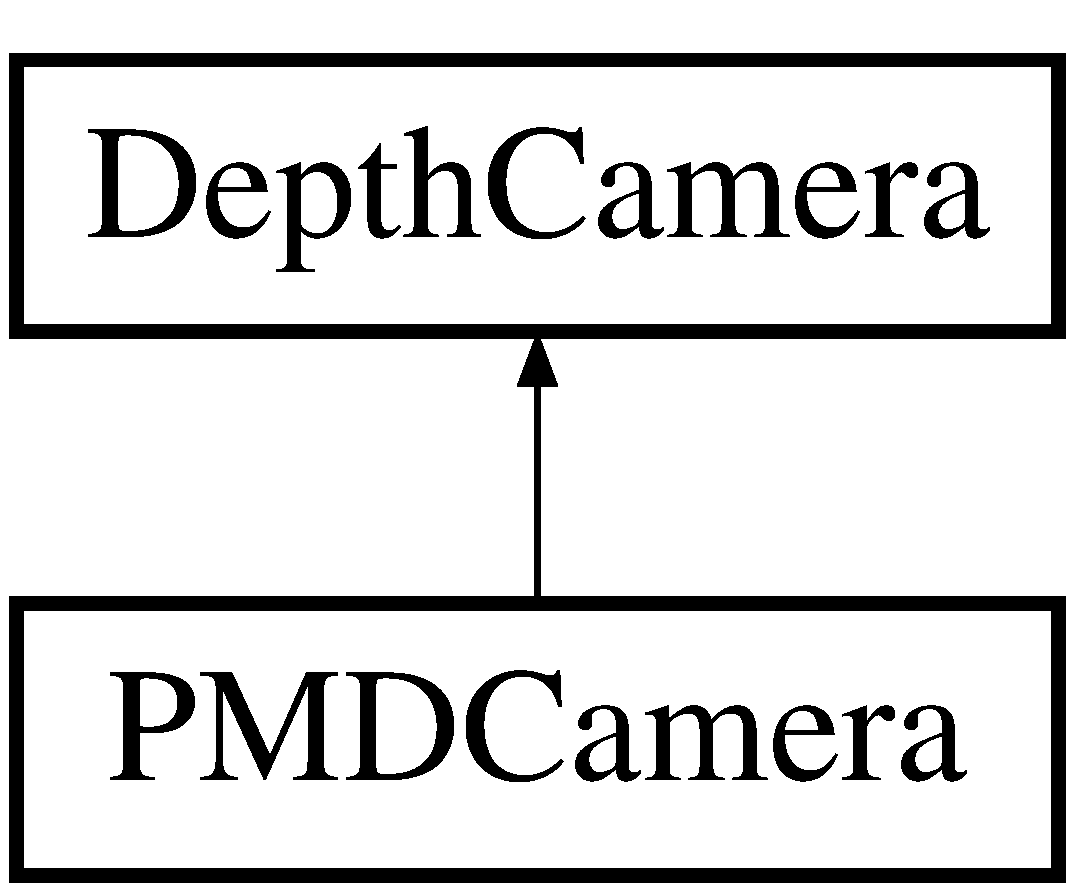
\includegraphics[height=2.000000cm]{class_depth_camera}
\end{center}
\end{figure}
\subsection*{Public Member Functions}
\begin{DoxyCompactItemize}
\item 
virtual void \hyperlink{class_depth_camera_abae1b9f37a00b17f00ff983ebb43ffc5}{update} ()=0
\begin{DoxyCompactList}\small\item\em Update the depth camera by one frame. \end{DoxyCompactList}\item 
virtual void \hyperlink{class_depth_camera_aaf7c09a863e906f61104f23af10a8597}{destroy\+Instance} ()=0
\begin{DoxyCompactList}\small\item\em Closes and exists the depth camera. \end{DoxyCompactList}\item 
void \hyperlink{class_depth_camera_a009719ec313de883b617903360bdf519}{compute\+Clusters} (double max\+\_\+distance, double min\+\_\+size)
\begin{DoxyCompactList}\small\item\em Performs euclidean clustering to separate discrete objects in the input point cloud. \end{DoxyCompactList}\item 
bool \hyperlink{class_depth_camera_a21cf887a447d2cdfda6ac907662c55fe}{read\+Image} (std\+::string source)
\begin{DoxyCompactList}\small\item\em Reads a sample frame from file. \end{DoxyCompactList}\item 
bool \hyperlink{class_depth_camera_a599dceaab9e673762b9ab76cf1e4f413}{write\+Image} (std\+::string destination)
\begin{DoxyCompactList}\small\item\em Writes the current frame into file. \end{DoxyCompactList}\item 
void \hyperlink{class_depth_camera_adc06db6509cc5f47de1e168f56bf41fa}{remove\+Noise} ()
\begin{DoxyCompactList}\small\item\em Removes noise from the X\+Y\+Z\+Map based on confidence provided in the Amp\+Map and Flag\+Map. \end{DoxyCompactList}\item 
void \hyperlink{class_depth_camera_a8f38ced63dcfb0c4c56cb7d4e940bcd8}{remove\+Points} (std\+::vector$<$ cv\+::\+Point2i $>$ points)
\begin{DoxyCompactList}\small\item\em Removes all points defined by the coordinates in the points vector from the X\+Y\+Z\+Map. \end{DoxyCompactList}\item 
cv\+::\+Mat \hyperlink{class_depth_camera_a0c295c5a0696550f453b1c8cd0fcb188}{get\+X\+Y\+Z\+Map} ()
\begin{DoxyCompactList}\small\item\em Return the current X\+Y\+Z\+Map. \end{DoxyCompactList}\item 
cv\+::\+Mat \hyperlink{class_depth_camera_a8211704726722a1be3d9b2aeeeffcf09}{get\+Amp\+Map} ()
\begin{DoxyCompactList}\small\item\em Return the current Amp\+Map. \end{DoxyCompactList}\item 
cv\+::\+Mat \hyperlink{class_depth_camera_a348cd41559a416a61780073f5369b032}{get\+Flag\+Map} ()
\begin{DoxyCompactList}\small\item\em Return the current Flag\+Map. \end{DoxyCompactList}\item 
int \hyperlink{class_depth_camera_a59fa917e64c6c67248787ba2cba3654b}{get\+Width} ()
\begin{DoxyCompactList}\small\item\em Returns the width of the frame in pixels. \end{DoxyCompactList}\item 
int \hyperlink{class_depth_camera_a430070d82a2bfc2583fd8290ca7bb8d6}{get\+Height} ()
\begin{DoxyCompactList}\small\item\em Returns the height of the frame in pixels. \end{DoxyCompactList}\item 
std\+::vector$<$ cv\+::\+Mat $>$ \hyperlink{class_depth_camera_a18d88b8df2a08c9c167207fea587d66e}{get\+Clusters} ()
\begin{DoxyCompactList}\small\item\em Returns all the clusters (discrete objects) in the current frame. \end{DoxyCompactList}\end{DoxyCompactItemize}
\subsection*{Public Attributes}
\begin{DoxyCompactItemize}
\item 
bool \hyperlink{class_depth_camera_a28f1ed73b3be887b3da06334416ac91a}{bad\+Input}
\end{DoxyCompactItemize}
\subsection*{Protected Member Functions}
\begin{DoxyCompactItemize}
\item 
void \hyperlink{class_depth_camera_a02f2fbde7cf4a340ace92278c89c66ef}{initilize\+Images} ()
\begin{DoxyCompactList}\small\item\em Initializes all variables used by the generic depth camera. \end{DoxyCompactList}\item 
void \hyperlink{class_depth_camera_acebcf84d24ce5bfd0b1392547dc79eb1}{flood\+Fill} (int x, int y, cv\+::\+Mat \&z\+Map, cv\+::\+Mat \&mask, double max\+\_\+distance)
\begin{DoxyCompactList}\small\item\em Performs floodfill starting from seed point (x,y). \end{DoxyCompactList}\item 
bool \hyperlink{class_depth_camera_ab24ac78c2cf29b0410c3d5e0dfc9a243}{close\+Enough} (int x, int y, cv\+::\+Mat \&depth\+Map, int num\+\_\+neighbors, double max\+\_\+distance)
\begin{DoxyCompactList}\small\item\em Analyze the candidate point with its neighbors to determine whether they belong to the same cluster. \end{DoxyCompactList}\end{DoxyCompactItemize}
\subsection*{Protected Attributes}
\begin{DoxyCompactItemize}
\item 
cv\+::\+Mat \hyperlink{class_depth_camera_a10123e69a9879a27a2c5ae434a916a5e}{xyz\+Map}
\begin{DoxyCompactList}\small\item\em Stores the (x,y,z) data of every point in the observable world. \end{DoxyCompactList}\item 
cv\+::\+Mat \hyperlink{class_depth_camera_a067d5cd9eedcdaa95cc440e7381fdb9c}{amp\+Map}
\begin{DoxyCompactList}\small\item\em Stores the confidence value of each corresponding point in the world. \end{DoxyCompactList}\item 
cv\+::\+Mat \hyperlink{class_depth_camera_a5b6e685ea92518f7deeb317ff6d0358f}{flag\+Map}
\begin{DoxyCompactList}\small\item\em Stores additional information about the points in the world. \end{DoxyCompactList}\item 
std\+::vector$<$ cv\+::\+Mat $>$ \hyperlink{class_depth_camera_a333347ab312906b2196596b078fc98b4}{clusters}
\begin{DoxyCompactList}\small\item\em Stores the each individual cluster in its individual X\+Y\+Z\+Map. \end{DoxyCompactList}\item 
double \hyperlink{class_depth_camera_a4a2bb91ca2e9be53a53c4a6dcf0e1677}{C\+O\+N\+F\+I\+D\+E\+N\+C\+E\+\_\+\+T\+H\+R\+E\+S\+H\+H\+O\+LD}
\begin{DoxyCompactList}\small\item\em Value that determines the validity of a point in respect to the amp\+Map. \end{DoxyCompactList}\item 
int \hyperlink{class_depth_camera_af7eb5186ae7366de110bb5b08803e11d}{I\+N\+V\+A\+L\+I\+D\+\_\+\+F\+L\+A\+G\+\_\+\+V\+A\+L\+UE}
\begin{DoxyCompactList}\small\item\em Value that determines the validity of a point in respect to the flag\+Map. \end{DoxyCompactList}\item 
int \hyperlink{class_depth_camera_a6e72272880679c710fb4aaeedf1d8309}{X\+\_\+\+D\+I\+M\+E\+N\+S\+I\+ON} = 176
\begin{DoxyCompactList}\small\item\em The image width resolution (pixels) that the depth sensor produces. \end{DoxyCompactList}\item 
int \hyperlink{class_depth_camera_a9c69a2e4d68fc09737317a638ad71f4a}{Y\+\_\+\+D\+I\+M\+E\+N\+S\+I\+ON} = 120
\begin{DoxyCompactList}\small\item\em The image height resolution (pixels) that the depth sensor produces. \end{DoxyCompactList}\end{DoxyCompactItemize}


\subsection{Detailed Description}
Class defining general behavior of a depth camera. 

Any depth camera should be able to generate a X\+Y\+X\+Map, Amp\+Map (confidence), and Flag\+Map. 

\subsection{Member Function Documentation}
\hypertarget{class_depth_camera_ab24ac78c2cf29b0410c3d5e0dfc9a243}{}\label{class_depth_camera_ab24ac78c2cf29b0410c3d5e0dfc9a243} 
\index{Depth\+Camera@{Depth\+Camera}!close\+Enough@{close\+Enough}}
\index{close\+Enough@{close\+Enough}!Depth\+Camera@{Depth\+Camera}}
\subsubsection{\texorpdfstring{close\+Enough()}{closeEnough()}}
{\footnotesize\ttfamily bool Depth\+Camera\+::close\+Enough (\begin{DoxyParamCaption}\item[{int}]{x,  }\item[{int}]{y,  }\item[{cv\+::\+Mat \&}]{depth\+Map,  }\item[{int}]{num\+\_\+neighbors,  }\item[{double}]{max\+\_\+distance }\end{DoxyParamCaption})\hspace{0.3cm}{\ttfamily [protected]}}



Analyze the candidate point with its neighbors to determine whether they belong to the same cluster. 


\begin{DoxyParams}[1]{Parameters}
 & {\em x} & x-\/coordinate of the candidate point \\
\hline
 & {\em y} & y-\/coordinate of the candidate point \\
\hline
\mbox{\tt in}  & {\em depth\+Map} & the xyz\+Map point cloud of the scene \\
\hline
 & {\em num\+\_\+neighbors} & the number of neighbors to consider \\
\hline
 & {\em max\+\_\+distance} & the maximum euclidean distance allowed between neighbors \\
\hline
\end{DoxyParams}
\hypertarget{class_depth_camera_a009719ec313de883b617903360bdf519}{}\label{class_depth_camera_a009719ec313de883b617903360bdf519} 
\index{Depth\+Camera@{Depth\+Camera}!compute\+Clusters@{compute\+Clusters}}
\index{compute\+Clusters@{compute\+Clusters}!Depth\+Camera@{Depth\+Camera}}
\subsubsection{\texorpdfstring{compute\+Clusters()}{computeClusters()}}
{\footnotesize\ttfamily void Depth\+Camera\+::compute\+Clusters (\begin{DoxyParamCaption}\item[{double}]{max\+\_\+distance,  }\item[{double}]{min\+\_\+size }\end{DoxyParamCaption})}



Performs euclidean clustering to separate discrete objects in the input point cloud. 


\begin{DoxyParams}{Parameters}
{\em max\+\_\+distance} & the maximum allowed distance to be clustered \\
\hline
{\em min\+\_\+size} & the minimum number of points a valid cluster should have \\
\hline
\end{DoxyParams}
\hypertarget{class_depth_camera_aaf7c09a863e906f61104f23af10a8597}{}\label{class_depth_camera_aaf7c09a863e906f61104f23af10a8597} 
\index{Depth\+Camera@{Depth\+Camera}!destroy\+Instance@{destroy\+Instance}}
\index{destroy\+Instance@{destroy\+Instance}!Depth\+Camera@{Depth\+Camera}}
\subsubsection{\texorpdfstring{destroy\+Instance()}{destroyInstance()}}
{\footnotesize\ttfamily virtual void Depth\+Camera\+::destroy\+Instance (\begin{DoxyParamCaption}{ }\end{DoxyParamCaption})\hspace{0.3cm}{\ttfamily [pure virtual]}}



Closes and exists the depth camera. 

This function should be overriden with a concrete implementation depending on the specific depth camera 

Implemented in \hyperlink{class_p_m_d_camera_a13090aeffb98e1440e715a93e67d3c0e}{P\+M\+D\+Camera}.

\hypertarget{class_depth_camera_acebcf84d24ce5bfd0b1392547dc79eb1}{}\label{class_depth_camera_acebcf84d24ce5bfd0b1392547dc79eb1} 
\index{Depth\+Camera@{Depth\+Camera}!flood\+Fill@{flood\+Fill}}
\index{flood\+Fill@{flood\+Fill}!Depth\+Camera@{Depth\+Camera}}
\subsubsection{\texorpdfstring{flood\+Fill()}{floodFill()}}
{\footnotesize\ttfamily void Depth\+Camera\+::flood\+Fill (\begin{DoxyParamCaption}\item[{int}]{x,  }\item[{int}]{y,  }\item[{cv\+::\+Mat \&}]{z\+Map,  }\item[{cv\+::\+Mat \&}]{mask,  }\item[{double}]{max\+\_\+distance }\end{DoxyParamCaption})\hspace{0.3cm}{\ttfamily [protected]}}



Performs floodfill starting from seed point (x,y). 


\begin{DoxyParams}[1]{Parameters}
 & {\em x} & x-\/coordinate of the seed point \\
\hline
 & {\em y} & y-\/coordinate of the seed point \\
\hline
\mbox{\tt in}  & {\em z\+Map} & the xyz\+Map point cloud \\
\hline
\mbox{\tt out}  & {\em mask} & the resulting region of the floodfill \\
\hline
 & {\em max\+\_\+distance} & the maximum euclidean distance allowed between neighbors \\
\hline
\end{DoxyParams}
\hypertarget{class_depth_camera_a8211704726722a1be3d9b2aeeeffcf09}{}\label{class_depth_camera_a8211704726722a1be3d9b2aeeeffcf09} 
\index{Depth\+Camera@{Depth\+Camera}!get\+Amp\+Map@{get\+Amp\+Map}}
\index{get\+Amp\+Map@{get\+Amp\+Map}!Depth\+Camera@{Depth\+Camera}}
\subsubsection{\texorpdfstring{get\+Amp\+Map()}{getAmpMap()}}
{\footnotesize\ttfamily cv\+::\+Mat Depth\+Camera\+::get\+Amp\+Map (\begin{DoxyParamCaption}{ }\end{DoxyParamCaption})}



Return the current Amp\+Map. 

\hypertarget{class_depth_camera_a18d88b8df2a08c9c167207fea587d66e}{}\label{class_depth_camera_a18d88b8df2a08c9c167207fea587d66e} 
\index{Depth\+Camera@{Depth\+Camera}!get\+Clusters@{get\+Clusters}}
\index{get\+Clusters@{get\+Clusters}!Depth\+Camera@{Depth\+Camera}}
\subsubsection{\texorpdfstring{get\+Clusters()}{getClusters()}}
{\footnotesize\ttfamily std\+::vector$<$ cv\+::\+Mat $>$ Depth\+Camera\+::get\+Clusters (\begin{DoxyParamCaption}{ }\end{DoxyParamCaption})}



Returns all the clusters (discrete objects) in the current frame. 

\begin{DoxySeeAlso}{See also}
\hyperlink{class_depth_camera_a009719ec313de883b617903360bdf519}{compute\+Clusters} 
\end{DoxySeeAlso}
\begin{DoxyReturn}{Returns}
vector of matrixes with each matrix corresponding to a cluster in no particular order 
\end{DoxyReturn}
\hypertarget{class_depth_camera_a348cd41559a416a61780073f5369b032}{}\label{class_depth_camera_a348cd41559a416a61780073f5369b032} 
\index{Depth\+Camera@{Depth\+Camera}!get\+Flag\+Map@{get\+Flag\+Map}}
\index{get\+Flag\+Map@{get\+Flag\+Map}!Depth\+Camera@{Depth\+Camera}}
\subsubsection{\texorpdfstring{get\+Flag\+Map()}{getFlagMap()}}
{\footnotesize\ttfamily cv\+::\+Mat Depth\+Camera\+::get\+Flag\+Map (\begin{DoxyParamCaption}{ }\end{DoxyParamCaption})}



Return the current Flag\+Map. 

\hypertarget{class_depth_camera_a430070d82a2bfc2583fd8290ca7bb8d6}{}\label{class_depth_camera_a430070d82a2bfc2583fd8290ca7bb8d6} 
\index{Depth\+Camera@{Depth\+Camera}!get\+Height@{get\+Height}}
\index{get\+Height@{get\+Height}!Depth\+Camera@{Depth\+Camera}}
\subsubsection{\texorpdfstring{get\+Height()}{getHeight()}}
{\footnotesize\ttfamily int Depth\+Camera\+::get\+Height (\begin{DoxyParamCaption}{ }\end{DoxyParamCaption})}



Returns the height of the frame in pixels. 

\hypertarget{class_depth_camera_a59fa917e64c6c67248787ba2cba3654b}{}\label{class_depth_camera_a59fa917e64c6c67248787ba2cba3654b} 
\index{Depth\+Camera@{Depth\+Camera}!get\+Width@{get\+Width}}
\index{get\+Width@{get\+Width}!Depth\+Camera@{Depth\+Camera}}
\subsubsection{\texorpdfstring{get\+Width()}{getWidth()}}
{\footnotesize\ttfamily int Depth\+Camera\+::get\+Width (\begin{DoxyParamCaption}{ }\end{DoxyParamCaption})}



Returns the width of the frame in pixels. 

\hypertarget{class_depth_camera_a0c295c5a0696550f453b1c8cd0fcb188}{}\label{class_depth_camera_a0c295c5a0696550f453b1c8cd0fcb188} 
\index{Depth\+Camera@{Depth\+Camera}!get\+X\+Y\+Z\+Map@{get\+X\+Y\+Z\+Map}}
\index{get\+X\+Y\+Z\+Map@{get\+X\+Y\+Z\+Map}!Depth\+Camera@{Depth\+Camera}}
\subsubsection{\texorpdfstring{get\+X\+Y\+Z\+Map()}{getXYZMap()}}
{\footnotesize\ttfamily cv\+::\+Mat Depth\+Camera\+::get\+X\+Y\+Z\+Map (\begin{DoxyParamCaption}{ }\end{DoxyParamCaption})}



Return the current X\+Y\+Z\+Map. 

\hypertarget{class_depth_camera_a02f2fbde7cf4a340ace92278c89c66ef}{}\label{class_depth_camera_a02f2fbde7cf4a340ace92278c89c66ef} 
\index{Depth\+Camera@{Depth\+Camera}!initilize\+Images@{initilize\+Images}}
\index{initilize\+Images@{initilize\+Images}!Depth\+Camera@{Depth\+Camera}}
\subsubsection{\texorpdfstring{initilize\+Images()}{initilizeImages()}}
{\footnotesize\ttfamily void Depth\+Camera\+::initilize\+Images (\begin{DoxyParamCaption}{ }\end{DoxyParamCaption})\hspace{0.3cm}{\ttfamily [protected]}}



Initializes all variables used by the generic depth camera. 

Sets xyz\+Map, amp\+Map, flag\+Map, and clusters to empty \hypertarget{class_depth_camera_a21cf887a447d2cdfda6ac907662c55fe}{}\label{class_depth_camera_a21cf887a447d2cdfda6ac907662c55fe} 
\index{Depth\+Camera@{Depth\+Camera}!read\+Image@{read\+Image}}
\index{read\+Image@{read\+Image}!Depth\+Camera@{Depth\+Camera}}
\subsubsection{\texorpdfstring{read\+Image()}{readImage()}}
{\footnotesize\ttfamily bool Depth\+Camera\+::read\+Image (\begin{DoxyParamCaption}\item[{std\+::string}]{source }\end{DoxyParamCaption})}



Reads a sample frame from file. 


\begin{DoxyParams}{Parameters}
{\em source} & the directory which the frame file is stored \\
\hline
\end{DoxyParams}
\hypertarget{class_depth_camera_adc06db6509cc5f47de1e168f56bf41fa}{}\label{class_depth_camera_adc06db6509cc5f47de1e168f56bf41fa} 
\index{Depth\+Camera@{Depth\+Camera}!remove\+Noise@{remove\+Noise}}
\index{remove\+Noise@{remove\+Noise}!Depth\+Camera@{Depth\+Camera}}
\subsubsection{\texorpdfstring{remove\+Noise()}{removeNoise()}}
{\footnotesize\ttfamily void Depth\+Camera\+::remove\+Noise (\begin{DoxyParamCaption}{ }\end{DoxyParamCaption})}



Removes noise from the X\+Y\+Z\+Map based on confidence provided in the Amp\+Map and Flag\+Map. 

\hypertarget{class_depth_camera_a8f38ced63dcfb0c4c56cb7d4e940bcd8}{}\label{class_depth_camera_a8f38ced63dcfb0c4c56cb7d4e940bcd8} 
\index{Depth\+Camera@{Depth\+Camera}!remove\+Points@{remove\+Points}}
\index{remove\+Points@{remove\+Points}!Depth\+Camera@{Depth\+Camera}}
\subsubsection{\texorpdfstring{remove\+Points()}{removePoints()}}
{\footnotesize\ttfamily void Depth\+Camera\+::remove\+Points (\begin{DoxyParamCaption}\item[{std\+::vector$<$ cv\+::\+Point2i $>$}]{points }\end{DoxyParamCaption})}



Removes all points defined by the coordinates in the points vector from the X\+Y\+Z\+Map. 


\begin{DoxyParams}[1]{Parameters}
\mbox{\tt in}  & {\em points} & the list of coordinates where data from the X\+Y\+Z\+Map should be removed \\
\hline
\end{DoxyParams}
\hypertarget{class_depth_camera_abae1b9f37a00b17f00ff983ebb43ffc5}{}\label{class_depth_camera_abae1b9f37a00b17f00ff983ebb43ffc5} 
\index{Depth\+Camera@{Depth\+Camera}!update@{update}}
\index{update@{update}!Depth\+Camera@{Depth\+Camera}}
\subsubsection{\texorpdfstring{update()}{update()}}
{\footnotesize\ttfamily virtual void Depth\+Camera\+::update (\begin{DoxyParamCaption}{ }\end{DoxyParamCaption})\hspace{0.3cm}{\ttfamily [pure virtual]}}



Update the depth camera by one frame. 

This function should be overriden with a concrete implementation depending on the specific depth camera 

Implemented in \hyperlink{class_p_m_d_camera_aa6cb9398f9635436b4384ee2043def40}{P\+M\+D\+Camera}.

\hypertarget{class_depth_camera_a599dceaab9e673762b9ab76cf1e4f413}{}\label{class_depth_camera_a599dceaab9e673762b9ab76cf1e4f413} 
\index{Depth\+Camera@{Depth\+Camera}!write\+Image@{write\+Image}}
\index{write\+Image@{write\+Image}!Depth\+Camera@{Depth\+Camera}}
\subsubsection{\texorpdfstring{write\+Image()}{writeImage()}}
{\footnotesize\ttfamily bool Depth\+Camera\+::write\+Image (\begin{DoxyParamCaption}\item[{std\+::string}]{destination }\end{DoxyParamCaption})}



Writes the current frame into file. 


\begin{DoxyParams}{Parameters}
{\em destination} & the directory which the frame should be written to \\
\hline
\end{DoxyParams}


\subsection{Member Data Documentation}
\hypertarget{class_depth_camera_a067d5cd9eedcdaa95cc440e7381fdb9c}{}\label{class_depth_camera_a067d5cd9eedcdaa95cc440e7381fdb9c} 
\index{Depth\+Camera@{Depth\+Camera}!amp\+Map@{amp\+Map}}
\index{amp\+Map@{amp\+Map}!Depth\+Camera@{Depth\+Camera}}
\subsubsection{\texorpdfstring{amp\+Map}{ampMap}}
{\footnotesize\ttfamily cv\+::\+Mat Depth\+Camera\+::amp\+Map\hspace{0.3cm}{\ttfamily [protected]}}



Stores the confidence value of each corresponding point in the world. 

Matrix type C\+V\+\_\+32\+F\+C1 \hypertarget{class_depth_camera_a28f1ed73b3be887b3da06334416ac91a}{}\label{class_depth_camera_a28f1ed73b3be887b3da06334416ac91a} 
\index{Depth\+Camera@{Depth\+Camera}!bad\+Input@{bad\+Input}}
\index{bad\+Input@{bad\+Input}!Depth\+Camera@{Depth\+Camera}}
\subsubsection{\texorpdfstring{bad\+Input}{badInput}}
{\footnotesize\ttfamily bool Depth\+Camera\+::bad\+Input}

\hypertarget{class_depth_camera_a333347ab312906b2196596b078fc98b4}{}\label{class_depth_camera_a333347ab312906b2196596b078fc98b4} 
\index{Depth\+Camera@{Depth\+Camera}!clusters@{clusters}}
\index{clusters@{clusters}!Depth\+Camera@{Depth\+Camera}}
\subsubsection{\texorpdfstring{clusters}{clusters}}
{\footnotesize\ttfamily std\+::vector$<$cv\+::\+Mat$>$ Depth\+Camera\+::clusters\hspace{0.3cm}{\ttfamily [protected]}}



Stores the each individual cluster in its individual X\+Y\+Z\+Map. 

\hypertarget{class_depth_camera_a4a2bb91ca2e9be53a53c4a6dcf0e1677}{}\label{class_depth_camera_a4a2bb91ca2e9be53a53c4a6dcf0e1677} 
\index{Depth\+Camera@{Depth\+Camera}!C\+O\+N\+F\+I\+D\+E\+N\+C\+E\+\_\+\+T\+H\+R\+E\+S\+H\+H\+O\+LD@{C\+O\+N\+F\+I\+D\+E\+N\+C\+E\+\_\+\+T\+H\+R\+E\+S\+H\+H\+O\+LD}}
\index{C\+O\+N\+F\+I\+D\+E\+N\+C\+E\+\_\+\+T\+H\+R\+E\+S\+H\+H\+O\+LD@{C\+O\+N\+F\+I\+D\+E\+N\+C\+E\+\_\+\+T\+H\+R\+E\+S\+H\+H\+O\+LD}!Depth\+Camera@{Depth\+Camera}}
\subsubsection{\texorpdfstring{C\+O\+N\+F\+I\+D\+E\+N\+C\+E\+\_\+\+T\+H\+R\+E\+S\+H\+H\+O\+LD}{CONFIDENCE\_THRESHHOLD}}
{\footnotesize\ttfamily double Depth\+Camera\+::\+C\+O\+N\+F\+I\+D\+E\+N\+C\+E\+\_\+\+T\+H\+R\+E\+S\+H\+H\+O\+LD\hspace{0.3cm}{\ttfamily [protected]}}



Value that determines the validity of a point in respect to the amp\+Map. 

This value varies from sensor to sensor so it should be define when constructing child class \hypertarget{class_depth_camera_a5b6e685ea92518f7deeb317ff6d0358f}{}\label{class_depth_camera_a5b6e685ea92518f7deeb317ff6d0358f} 
\index{Depth\+Camera@{Depth\+Camera}!flag\+Map@{flag\+Map}}
\index{flag\+Map@{flag\+Map}!Depth\+Camera@{Depth\+Camera}}
\subsubsection{\texorpdfstring{flag\+Map}{flagMap}}
{\footnotesize\ttfamily cv\+::\+Mat Depth\+Camera\+::flag\+Map\hspace{0.3cm}{\ttfamily [protected]}}



Stores additional information about the points in the world. 

Matrix type C\+V\+\_\+8\+U\+C1 \hypertarget{class_depth_camera_af7eb5186ae7366de110bb5b08803e11d}{}\label{class_depth_camera_af7eb5186ae7366de110bb5b08803e11d} 
\index{Depth\+Camera@{Depth\+Camera}!I\+N\+V\+A\+L\+I\+D\+\_\+\+F\+L\+A\+G\+\_\+\+V\+A\+L\+UE@{I\+N\+V\+A\+L\+I\+D\+\_\+\+F\+L\+A\+G\+\_\+\+V\+A\+L\+UE}}
\index{I\+N\+V\+A\+L\+I\+D\+\_\+\+F\+L\+A\+G\+\_\+\+V\+A\+L\+UE@{I\+N\+V\+A\+L\+I\+D\+\_\+\+F\+L\+A\+G\+\_\+\+V\+A\+L\+UE}!Depth\+Camera@{Depth\+Camera}}
\subsubsection{\texorpdfstring{I\+N\+V\+A\+L\+I\+D\+\_\+\+F\+L\+A\+G\+\_\+\+V\+A\+L\+UE}{INVALID\_FLAG\_VALUE}}
{\footnotesize\ttfamily int Depth\+Camera\+::\+I\+N\+V\+A\+L\+I\+D\+\_\+\+F\+L\+A\+G\+\_\+\+V\+A\+L\+UE\hspace{0.3cm}{\ttfamily [protected]}}



Value that determines the validity of a point in respect to the flag\+Map. 

This value varies from sensor to sensor so it should be defined when constructing child class \hypertarget{class_depth_camera_a6e72272880679c710fb4aaeedf1d8309}{}\label{class_depth_camera_a6e72272880679c710fb4aaeedf1d8309} 
\index{Depth\+Camera@{Depth\+Camera}!X\+\_\+\+D\+I\+M\+E\+N\+S\+I\+ON@{X\+\_\+\+D\+I\+M\+E\+N\+S\+I\+ON}}
\index{X\+\_\+\+D\+I\+M\+E\+N\+S\+I\+ON@{X\+\_\+\+D\+I\+M\+E\+N\+S\+I\+ON}!Depth\+Camera@{Depth\+Camera}}
\subsubsection{\texorpdfstring{X\+\_\+\+D\+I\+M\+E\+N\+S\+I\+ON}{X\_DIMENSION}}
{\footnotesize\ttfamily int Depth\+Camera\+::\+X\+\_\+\+D\+I\+M\+E\+N\+S\+I\+ON = 176\hspace{0.3cm}{\ttfamily [protected]}}



The image width resolution (pixels) that the depth sensor produces. 

\hypertarget{class_depth_camera_a10123e69a9879a27a2c5ae434a916a5e}{}\label{class_depth_camera_a10123e69a9879a27a2c5ae434a916a5e} 
\index{Depth\+Camera@{Depth\+Camera}!xyz\+Map@{xyz\+Map}}
\index{xyz\+Map@{xyz\+Map}!Depth\+Camera@{Depth\+Camera}}
\subsubsection{\texorpdfstring{xyz\+Map}{xyzMap}}
{\footnotesize\ttfamily cv\+::\+Mat Depth\+Camera\+::xyz\+Map\hspace{0.3cm}{\ttfamily [protected]}}



Stores the (x,y,z) data of every point in the observable world. 

Matrix type C\+V\+\_\+32\+F\+C3 \hypertarget{class_depth_camera_a9c69a2e4d68fc09737317a638ad71f4a}{}\label{class_depth_camera_a9c69a2e4d68fc09737317a638ad71f4a} 
\index{Depth\+Camera@{Depth\+Camera}!Y\+\_\+\+D\+I\+M\+E\+N\+S\+I\+ON@{Y\+\_\+\+D\+I\+M\+E\+N\+S\+I\+ON}}
\index{Y\+\_\+\+D\+I\+M\+E\+N\+S\+I\+ON@{Y\+\_\+\+D\+I\+M\+E\+N\+S\+I\+ON}!Depth\+Camera@{Depth\+Camera}}
\subsubsection{\texorpdfstring{Y\+\_\+\+D\+I\+M\+E\+N\+S\+I\+ON}{Y\_DIMENSION}}
{\footnotesize\ttfamily int Depth\+Camera\+::\+Y\+\_\+\+D\+I\+M\+E\+N\+S\+I\+ON = 120\hspace{0.3cm}{\ttfamily [protected]}}



The image height resolution (pixels) that the depth sensor produces. 



The documentation for this class was generated from the following files\+:\begin{DoxyCompactItemize}
\item 
\hyperlink{_depth_camera_8h}{Depth\+Camera.\+h}\item 
\hyperlink{_depth_camera_8cpp}{Depth\+Camera.\+cpp}\end{DoxyCompactItemize}

\hypertarget{class_hand}{}\section{Hand Class Reference}
\label{class_hand}\index{Hand@{Hand}}


{\ttfamily \#include $<$Hand.\+h$>$}

\subsection*{Public Member Functions}
\begin{DoxyCompactItemize}
\item 
\hyperlink{class_hand_aa733faf150351c640fc7d1bf460b07e9}{Hand} ()
\begin{DoxyCompactList}\small\item\em Default constructor for a hand object. \end{DoxyCompactList}\item 
\hyperlink{class_hand_abc73f91de5c25f023c7411fb353f8509}{Hand} (cv\+::\+Mat xyz\+Map, float angle\+\_\+treshhold, int cluster\+\_\+thresh=30)
\begin{DoxyCompactList}\small\item\em Constructs a hand object based on point cloud and constraints. \end{DoxyCompactList}\item 
\hyperlink{class_hand_a7ff29a6f23f98c5e57f44d23a76912be}{$\sim$\+Hand} ()
\begin{DoxyCompactList}\small\item\em Deconstructor for the hand object. \end{DoxyCompactList}\item 
bool \hyperlink{class_hand_aad89c3e47921cb0c39430f4501238088}{touch\+Object} (std\+::vector$<$ double $>$ \&equation, const double threshold)
\begin{DoxyCompactList}\small\item\em Determine whether one of the fingers is in contact with a tracked object. \end{DoxyCompactList}\end{DoxyCompactItemize}
\subsection*{Public Attributes}
\begin{DoxyCompactItemize}
\item 
int \hyperlink{class_hand_a8fee584c52a9c38a8c9500b86859a610}{C\+L\+U\+S\+T\+E\+R\+\_\+\+T\+H\+R\+E\+S\+H\+O\+LD}
\begin{DoxyCompactList}\small\item\em Maximum allowable distance between adjacent finger tips. \end{DoxyCompactList}\item 
std\+::vector$<$ cv\+::\+Vec3f $>$ \hyperlink{class_hand_afb4b29e1aaca7d0779af899a9eeaa21d}{fingers\+\_\+xyz}
\begin{DoxyCompactList}\small\item\em (x,y,z) position of all detected finger tips \end{DoxyCompactList}\item 
std\+::vector$<$ cv\+::\+Point2i $>$ \hyperlink{class_hand_a4539e1c12c9c3ef9218d4e96c3aebd4b}{fingers\+\_\+ij}
\begin{DoxyCompactList}\small\item\em (i,j) coordinates of all detected finger tips \end{DoxyCompactList}\item 
cv\+::\+Vec3f \hyperlink{class_hand_af1d336666d556ea9d900bdd7bae6b88c}{centroid\+\_\+xyz}
\begin{DoxyCompactList}\small\item\em (x,y,z) position of hand centroid \end{DoxyCompactList}\item 
cv\+::\+Point2i \hyperlink{class_hand_a1b7c44a205ea0ec4a89a24abc8ce84af}{centroid\+\_\+ij}
\begin{DoxyCompactList}\small\item\em (i,j) coordinates of hand centroid \end{DoxyCompactList}\item 
std\+::vector$<$ cv\+::\+Vec3f $>$ \hyperlink{class_hand_aad21d7ee1c845701e47c37d6c5ac96d5}{defects\+\_\+xyz}
\begin{DoxyCompactList}\small\item\em (x,y,z) position of detected defects \end{DoxyCompactList}\item 
std\+::vector$<$ cv\+::\+Point2i $>$ \hyperlink{class_hand_a7d0281af3003f2f935115e5956056415}{defects\+\_\+ij}
\begin{DoxyCompactList}\small\item\em (i,j) position of detected defects \end{DoxyCompactList}\end{DoxyCompactItemize}
\subsection*{Private Member Functions}
\begin{DoxyCompactItemize}
\item 
std\+::vector$<$ cv\+::\+Point $>$ \hyperlink{class_hand_a836fa2da6d128e2db7eca7e4965d0a2d}{find\+Complex\+Contour} (std\+::vector$<$ std\+::vector$<$ cv\+::\+Point $>$ $>$ contours)
\begin{DoxyCompactList}\small\item\em Find the contour with max number of vertices. \end{DoxyCompactList}\item 
std\+::vector$<$ cv\+::\+Point $>$ \hyperlink{class_hand_ad7b1c8745ec41d551945e75e75961f85}{cluster\+Convex\+Hull} (std\+::vector$<$ cv\+::\+Point $>$ convex\+Hull, int threshold)
\begin{DoxyCompactList}\small\item\em Groups vertices within a threshold and selects the median of each group. \end{DoxyCompactList}\item 
cv\+::\+Point \hyperlink{class_hand_ab089502dd52e8251c5a9efadac2784dd}{find\+Center} (std\+::vector$<$ cv\+::\+Point $>$ contour)
\begin{DoxyCompactList}\small\item\em Find the centroid of contour using 0th and 1st degree moments. \end{DoxyCompactList}\item 
void \hyperlink{class_hand_a0a58ac8e96eab17c99f820f0a4075275}{analyze\+Hand} (cv\+::\+Mat xyz\+Map)
\end{DoxyCompactItemize}
\subsection*{Private Attributes}
\begin{DoxyCompactItemize}
\item 
float \hyperlink{class_hand_aae06e06e724346861df0a7fdddcfc3c8}{A\+N\+G\+L\+E\+\_\+\+T\+H\+R\+E\+S\+H\+H\+O\+LD}
\end{DoxyCompactItemize}


\subsection{Constructor \& Destructor Documentation}
\hypertarget{class_hand_aa733faf150351c640fc7d1bf460b07e9}{}\label{class_hand_aa733faf150351c640fc7d1bf460b07e9} 
\index{Hand@{Hand}!Hand@{Hand}}
\index{Hand@{Hand}!Hand@{Hand}}
\subsubsection{\texorpdfstring{Hand()}{Hand()}\hspace{0.1cm}{\footnotesize\ttfamily [1/2]}}
{\footnotesize\ttfamily Hand\+::\+Hand (\begin{DoxyParamCaption}{ }\end{DoxyParamCaption})}



Default constructor for a hand object. 

\hypertarget{class_hand_abc73f91de5c25f023c7411fb353f8509}{}\label{class_hand_abc73f91de5c25f023c7411fb353f8509} 
\index{Hand@{Hand}!Hand@{Hand}}
\index{Hand@{Hand}!Hand@{Hand}}
\subsubsection{\texorpdfstring{Hand()}{Hand()}\hspace{0.1cm}{\footnotesize\ttfamily [2/2]}}
{\footnotesize\ttfamily Hand\+::\+Hand (\begin{DoxyParamCaption}\item[{cv\+::\+Mat}]{xyz\+Map,  }\item[{float}]{angle\+\_\+treshhold,  }\item[{int}]{cluster\+\_\+thresh = {\ttfamily 30} }\end{DoxyParamCaption})}



Constructs a hand object based on point cloud and constraints. 


\begin{DoxyParams}{Parameters}
{\em xyz\+Map} & Input point cloud containing only the hand (nothing else can be in this point cluod) \\
\hline
{\em angle\+\_\+treshhold} & Sharpest allowable angle formed by finger tip and neighboring defects \\
\hline
{\em cluster\+\_\+thresh} & Maximum allowable distance between two finger tips \\
\hline
\end{DoxyParams}
\hypertarget{class_hand_a7ff29a6f23f98c5e57f44d23a76912be}{}\label{class_hand_a7ff29a6f23f98c5e57f44d23a76912be} 
\index{Hand@{Hand}!````~Hand@{$\sim$\+Hand}}
\index{````~Hand@{$\sim$\+Hand}!Hand@{Hand}}
\subsubsection{\texorpdfstring{$\sim$\+Hand()}{~Hand()}}
{\footnotesize\ttfamily Hand\+::$\sim$\+Hand (\begin{DoxyParamCaption}{ }\end{DoxyParamCaption})}



Deconstructor for the hand object. 



\subsection{Member Function Documentation}
\hypertarget{class_hand_a0a58ac8e96eab17c99f820f0a4075275}{}\label{class_hand_a0a58ac8e96eab17c99f820f0a4075275} 
\index{Hand@{Hand}!analyze\+Hand@{analyze\+Hand}}
\index{analyze\+Hand@{analyze\+Hand}!Hand@{Hand}}
\subsubsection{\texorpdfstring{analyze\+Hand()}{analyzeHand()}}
{\footnotesize\ttfamily void Hand\+::analyze\+Hand (\begin{DoxyParamCaption}\item[{cv\+::\+Mat}]{xyz\+Map }\end{DoxyParamCaption})\hspace{0.3cm}{\ttfamily [private]}}

\hypertarget{class_hand_ad7b1c8745ec41d551945e75e75961f85}{}\label{class_hand_ad7b1c8745ec41d551945e75e75961f85} 
\index{Hand@{Hand}!cluster\+Convex\+Hull@{cluster\+Convex\+Hull}}
\index{cluster\+Convex\+Hull@{cluster\+Convex\+Hull}!Hand@{Hand}}
\subsubsection{\texorpdfstring{cluster\+Convex\+Hull()}{clusterConvexHull()}}
{\footnotesize\ttfamily std\+::vector$<$ cv\+::\+Point $>$ Hand\+::cluster\+Convex\+Hull (\begin{DoxyParamCaption}\item[{std\+::vector$<$ cv\+::\+Point $>$}]{convex\+Hull,  }\item[{int}]{threshold }\end{DoxyParamCaption})\hspace{0.3cm}{\ttfamily [private]}}



Groups vertices within a threshold and selects the median of each group. 

\hypertarget{class_hand_ab089502dd52e8251c5a9efadac2784dd}{}\label{class_hand_ab089502dd52e8251c5a9efadac2784dd} 
\index{Hand@{Hand}!find\+Center@{find\+Center}}
\index{find\+Center@{find\+Center}!Hand@{Hand}}
\subsubsection{\texorpdfstring{find\+Center()}{findCenter()}}
{\footnotesize\ttfamily cv\+::\+Point Hand\+::find\+Center (\begin{DoxyParamCaption}\item[{std\+::vector$<$ cv\+::\+Point $>$}]{contour }\end{DoxyParamCaption})\hspace{0.3cm}{\ttfamily [private]}}



Find the centroid of contour using 0th and 1st degree moments. 

\hypertarget{class_hand_a836fa2da6d128e2db7eca7e4965d0a2d}{}\label{class_hand_a836fa2da6d128e2db7eca7e4965d0a2d} 
\index{Hand@{Hand}!find\+Complex\+Contour@{find\+Complex\+Contour}}
\index{find\+Complex\+Contour@{find\+Complex\+Contour}!Hand@{Hand}}
\subsubsection{\texorpdfstring{find\+Complex\+Contour()}{findComplexContour()}}
{\footnotesize\ttfamily std\+::vector$<$ cv\+::\+Point $>$ Hand\+::find\+Complex\+Contour (\begin{DoxyParamCaption}\item[{std\+::vector$<$ std\+::vector$<$ cv\+::\+Point $>$ $>$}]{contours }\end{DoxyParamCaption})\hspace{0.3cm}{\ttfamily [private]}}



Find the contour with max number of vertices. 

\hypertarget{class_hand_aad89c3e47921cb0c39430f4501238088}{}\label{class_hand_aad89c3e47921cb0c39430f4501238088} 
\index{Hand@{Hand}!touch\+Object@{touch\+Object}}
\index{touch\+Object@{touch\+Object}!Hand@{Hand}}
\subsubsection{\texorpdfstring{touch\+Object()}{touchObject()}}
{\footnotesize\ttfamily bool Hand\+::touch\+Object (\begin{DoxyParamCaption}\item[{std\+::vector$<$ double $>$ \&}]{equation,  }\item[{const double}]{threshold }\end{DoxyParamCaption})}



Determine whether one of the fingers is in contact with a tracked object. 


\begin{DoxyParams}{Parameters}
{\em equation} & Regression equation of the object \\
\hline
{\em threshold} & Thickness of the plane modeled by the regression equation \\
\hline
\end{DoxyParams}
\begin{DoxyReturn}{Returns}
T\+R\+UE if hand is contacting a tracked object. F\+A\+L\+SE otherwise 
\end{DoxyReturn}


\subsection{Member Data Documentation}
\hypertarget{class_hand_aae06e06e724346861df0a7fdddcfc3c8}{}\label{class_hand_aae06e06e724346861df0a7fdddcfc3c8} 
\index{Hand@{Hand}!A\+N\+G\+L\+E\+\_\+\+T\+H\+R\+E\+S\+H\+H\+O\+LD@{A\+N\+G\+L\+E\+\_\+\+T\+H\+R\+E\+S\+H\+H\+O\+LD}}
\index{A\+N\+G\+L\+E\+\_\+\+T\+H\+R\+E\+S\+H\+H\+O\+LD@{A\+N\+G\+L\+E\+\_\+\+T\+H\+R\+E\+S\+H\+H\+O\+LD}!Hand@{Hand}}
\subsubsection{\texorpdfstring{A\+N\+G\+L\+E\+\_\+\+T\+H\+R\+E\+S\+H\+H\+O\+LD}{ANGLE\_THRESHHOLD}}
{\footnotesize\ttfamily float Hand\+::\+A\+N\+G\+L\+E\+\_\+\+T\+H\+R\+E\+S\+H\+H\+O\+LD\hspace{0.3cm}{\ttfamily [private]}}

\hypertarget{class_hand_a1b7c44a205ea0ec4a89a24abc8ce84af}{}\label{class_hand_a1b7c44a205ea0ec4a89a24abc8ce84af} 
\index{Hand@{Hand}!centroid\+\_\+ij@{centroid\+\_\+ij}}
\index{centroid\+\_\+ij@{centroid\+\_\+ij}!Hand@{Hand}}
\subsubsection{\texorpdfstring{centroid\+\_\+ij}{centroid\_ij}}
{\footnotesize\ttfamily cv\+::\+Point2i Hand\+::centroid\+\_\+ij}



(i,j) coordinates of hand centroid 

\hypertarget{class_hand_af1d336666d556ea9d900bdd7bae6b88c}{}\label{class_hand_af1d336666d556ea9d900bdd7bae6b88c} 
\index{Hand@{Hand}!centroid\+\_\+xyz@{centroid\+\_\+xyz}}
\index{centroid\+\_\+xyz@{centroid\+\_\+xyz}!Hand@{Hand}}
\subsubsection{\texorpdfstring{centroid\+\_\+xyz}{centroid\_xyz}}
{\footnotesize\ttfamily cv\+::\+Vec3f Hand\+::centroid\+\_\+xyz}



(x,y,z) position of hand centroid 

\hypertarget{class_hand_a8fee584c52a9c38a8c9500b86859a610}{}\label{class_hand_a8fee584c52a9c38a8c9500b86859a610} 
\index{Hand@{Hand}!C\+L\+U\+S\+T\+E\+R\+\_\+\+T\+H\+R\+E\+S\+H\+O\+LD@{C\+L\+U\+S\+T\+E\+R\+\_\+\+T\+H\+R\+E\+S\+H\+O\+LD}}
\index{C\+L\+U\+S\+T\+E\+R\+\_\+\+T\+H\+R\+E\+S\+H\+O\+LD@{C\+L\+U\+S\+T\+E\+R\+\_\+\+T\+H\+R\+E\+S\+H\+O\+LD}!Hand@{Hand}}
\subsubsection{\texorpdfstring{C\+L\+U\+S\+T\+E\+R\+\_\+\+T\+H\+R\+E\+S\+H\+O\+LD}{CLUSTER\_THRESHOLD}}
{\footnotesize\ttfamily int Hand\+::\+C\+L\+U\+S\+T\+E\+R\+\_\+\+T\+H\+R\+E\+S\+H\+O\+LD}



Maximum allowable distance between adjacent finger tips. 

\hypertarget{class_hand_a7d0281af3003f2f935115e5956056415}{}\label{class_hand_a7d0281af3003f2f935115e5956056415} 
\index{Hand@{Hand}!defects\+\_\+ij@{defects\+\_\+ij}}
\index{defects\+\_\+ij@{defects\+\_\+ij}!Hand@{Hand}}
\subsubsection{\texorpdfstring{defects\+\_\+ij}{defects\_ij}}
{\footnotesize\ttfamily std\+::vector$<$cv\+::\+Point2i$>$ Hand\+::defects\+\_\+ij}



(i,j) position of detected defects 

\hypertarget{class_hand_aad21d7ee1c845701e47c37d6c5ac96d5}{}\label{class_hand_aad21d7ee1c845701e47c37d6c5ac96d5} 
\index{Hand@{Hand}!defects\+\_\+xyz@{defects\+\_\+xyz}}
\index{defects\+\_\+xyz@{defects\+\_\+xyz}!Hand@{Hand}}
\subsubsection{\texorpdfstring{defects\+\_\+xyz}{defects\_xyz}}
{\footnotesize\ttfamily std\+::vector$<$cv\+::\+Vec3f$>$ Hand\+::defects\+\_\+xyz}



(x,y,z) position of detected defects 

\hypertarget{class_hand_a4539e1c12c9c3ef9218d4e96c3aebd4b}{}\label{class_hand_a4539e1c12c9c3ef9218d4e96c3aebd4b} 
\index{Hand@{Hand}!fingers\+\_\+ij@{fingers\+\_\+ij}}
\index{fingers\+\_\+ij@{fingers\+\_\+ij}!Hand@{Hand}}
\subsubsection{\texorpdfstring{fingers\+\_\+ij}{fingers\_ij}}
{\footnotesize\ttfamily std\+::vector$<$cv\+::\+Point2i$>$ Hand\+::fingers\+\_\+ij}



(i,j) coordinates of all detected finger tips 

\hypertarget{class_hand_afb4b29e1aaca7d0779af899a9eeaa21d}{}\label{class_hand_afb4b29e1aaca7d0779af899a9eeaa21d} 
\index{Hand@{Hand}!fingers\+\_\+xyz@{fingers\+\_\+xyz}}
\index{fingers\+\_\+xyz@{fingers\+\_\+xyz}!Hand@{Hand}}
\subsubsection{\texorpdfstring{fingers\+\_\+xyz}{fingers\_xyz}}
{\footnotesize\ttfamily std\+::vector$<$cv\+::\+Vec3f$>$ Hand\+::fingers\+\_\+xyz}



(x,y,z) position of all detected finger tips 



The documentation for this class was generated from the following files\+:\begin{DoxyCompactItemize}
\item 
\hyperlink{_hand_8h}{Hand.\+h}\item 
\hyperlink{_hand_8cpp}{Hand.\+cpp}\end{DoxyCompactItemize}

\hypertarget{class_plane}{}\section{Plane Class Reference}
\label{class_plane}\index{Plane@{Plane}}


Class defining a plane object.  




{\ttfamily \#include $<$Plane.\+h$>$}

\subsection*{Public Member Functions}
\begin{DoxyCompactItemize}
\item 
\hyperlink{class_plane_acac0d9c003e0ab10d07b146c3566a0c7}{Plane} ()
\item 
\hyperlink{class_plane_a94bc1ca29c305edb76676528b1a9465c}{Plane} (cv\+::\+Mat \&src)
\begin{DoxyCompactList}\small\item\em Constructs a plane object from a unsegemented xyz\+Map. \end{DoxyCompactList}\item 
\hyperlink{class_plane_a69abd86051c880dcb44b249ad10c4436}{$\sim$\+Plane} ()
\begin{DoxyCompactList}\small\item\em Deconstructs the plane object. \end{DoxyCompactList}\item 
void \hyperlink{class_plane_ab884c9687d63290912707f749adad115}{initialize\+Cloud} (cv\+::\+Mat \&src)
\begin{DoxyCompactList}\small\item\em Initializes all the required point clouds. \end{DoxyCompactList}\item 
pcl\+::\+Point\+Cloud$<$ pcl\+::\+Point\+X\+YZ $>$\+::Ptr \hyperlink{class_plane_a89c277f419ffb0e9d53f29127109465b}{get\+Cloud} ()
\begin{DoxyCompactList}\small\item\em Returns the P\+CL representation of the xyz\+Map. \end{DoxyCompactList}\item 
pcl\+::\+Point\+Cloud$<$ pcl\+::\+Point\+X\+YZ $>$\+::Ptr \hyperlink{class_plane_abad6f7c26005ad7ab847af5acaad9c31}{get\+Down\+Cloud} ()
\begin{DoxyCompactList}\small\item\em Returns the P\+CL representatino of a down sampled xyz\+Map. \end{DoxyCompactList}\item 
std\+::vector$<$ double $>$ \hyperlink{class_plane_aafedb091ba358d46d5203c4e0eb6e838}{get\+Plane\+Equation} ()
\begin{DoxyCompactList}\small\item\em Returns the planar regression equation of the identified plane. \end{DoxyCompactList}\item 
std\+::vector$<$ double $>$ \hyperlink{class_plane_ab82069a9be653b07a589374c03b2f436}{get\+Sphere\+Equation} ()
\begin{DoxyCompactList}\small\item\em Returns the sphereical regression equation of the identified plane. \end{DoxyCompactList}\item 
std\+::vector$<$ cv\+::\+Point2i $>$ \hyperlink{class_plane_a843717e035e2e6b4e03a8eece14098b1}{get\+Plane\+Indicies} ()
\begin{DoxyCompactList}\small\item\em Returns the (i,j) indices for which the plane appears on the xyz\+Map. \end{DoxyCompactList}\item 
std\+::vector$<$ cv\+::\+Point2i $>$ \hyperlink{class_plane_acd72c8d01f393ef78c4ed1f685d1d36d}{get\+Sphere\+Indices} ()
\begin{DoxyCompactList}\small\item\em Returns the (i,j) indices for which the plane appears on the xyz\+Map. \end{DoxyCompactList}\end{DoxyCompactItemize}
\subsection*{Public Attributes}
\begin{DoxyCompactItemize}
\item 
const int \hyperlink{class_plane_a1251f1df31bce7666494bfb6d069dd2e}{C\+L\+O\+U\+D\+\_\+\+S\+I\+Z\+E\+\_\+\+T\+H\+R\+E\+S\+H\+O\+LD} = 1000
\begin{DoxyCompactList}\small\item\em Maximum cloud size (pixel) allowed. \end{DoxyCompactList}\item 
const double \hyperlink{class_plane_ae0e9b28377ab03e577aa6588da269328}{R\+\_\+\+S\+Q\+U\+A\+R\+E\+D\+\_\+\+D\+I\+S\+T\+A\+N\+C\+E\+\_\+\+T\+H\+R\+E\+S\+H\+O\+LD} = 0.\+0005
\begin{DoxyCompactList}\small\item\em Maximum distance (mm) allowed between real point and regression equation. \end{DoxyCompactList}\end{DoxyCompactItemize}
\subsection*{Private Member Functions}
\begin{DoxyCompactItemize}
\item 
int \hyperlink{class_plane_a50f718840ac2c5cc3226ff66de2c60f6}{compute} ()
\begin{DoxyCompactList}\small\item\em Performs a series of computations to find the plane. \end{DoxyCompactList}\item 
void \hyperlink{class_plane_a5c856cf6a603473c68381d21a544d2a3}{calculate\+Normals} (pcl\+::\+Normal\+Estimation\+O\+MP$<$ pcl\+::\+Point\+X\+YZ, pcl\+::\+Normal $>$ normal\+\_\+estimator, pcl\+::search\+::\+Search$<$ pcl\+::\+Point\+X\+YZ $>$\+::Ptr tree)
\begin{DoxyCompactList}\small\item\em Computes the normals at every point. \end{DoxyCompactList}\item 
void \hyperlink{class_plane_afc8f76c6dc7223c7d681d69e427a3004}{voxel\+Downsample} ()
\begin{DoxyCompactList}\small\item\em Down samples the cloud via a median filter. \end{DoxyCompactList}\item 
void \hyperlink{class_plane_a08b35c23d8e0f3eea0db820163cda6e0}{region\+Grow} (pcl\+::\+Region\+Growing$<$ pcl\+::\+Point\+X\+YZ, pcl\+::\+Normal $>$ \&reg, pcl\+::search\+::\+Search$<$ pcl\+::\+Point\+X\+YZ $>$\+::Ptr tree)
\begin{DoxyCompactList}\small\item\em Aggregates points with like normals. \end{DoxyCompactList}\item 
void \hyperlink{class_plane_a503b1c82ae3a84d9bd88fbfa37a5e3be}{compute\+Plane\+L\+SE} (pcl\+::\+Point\+Indices \&ind)
\begin{DoxyCompactList}\small\item\em Compute a planar regression equation. \end{DoxyCompactList}\item 
void \hyperlink{class_plane_a60923e0c6d087076a234a9d5bd45d0fa}{compute\+Sphere\+L\+SE} (pcl\+::\+Point\+Indices \&ind)
\begin{DoxyCompactList}\small\item\em Compute a sphereical regression equation. \end{DoxyCompactList}\item 
int \hyperlink{class_plane_a24415419c0c06e83f2016246a8d2ee40}{compute\+Plane\+Indices} ()
\begin{DoxyCompactList}\small\item\em Compute all the (i,j) index of the plane points from the planar regression. \end{DoxyCompactList}\item 
int \hyperlink{class_plane_a279bfd98317431edcdefe43004bb257f}{compute\+Sphere\+Indices} ()
\begin{DoxyCompactList}\small\item\em Compute all the (i,j) index of the plane points from the sphereical regression. \end{DoxyCompactList}\item 
int \hyperlink{class_plane_a12c28b7eeb8cdef5451e2e90704e0673}{draw\+Sphere\+Regression\+Points} (cv\+::\+Mat \&output\+\_\+mat, cv\+::\+Mat \&input\+\_\+mat, std\+::vector$<$ double $>$ \&equation, const int row\+Size, const int col\+Size, const double threshold, bool clicked)
\end{DoxyCompactItemize}
\subsection*{Private Attributes}
\begin{DoxyCompactItemize}
\item 
pcl\+::\+Point\+Cloud$<$ pcl\+::\+Point\+X\+YZ $>$\+::Ptr $\ast$ \hyperlink{class_plane_a0b493693b28fb0cc74549fa24ded3721}{cloud}
\item 
pcl\+::\+Point\+Cloud$<$ pcl\+::\+Normal $>$\+::Ptr $\ast$ \hyperlink{class_plane_a28e30d6c24eaa6c4e1d57ea8c1a2d924}{normals}
\item 
pcl\+::\+Point\+Cloud$<$ pcl\+::\+Point\+X\+YZ $>$\+::Ptr $\ast$ \hyperlink{class_plane_ae4198f097fe1b58f10068f7bc0962c8c}{down\+\_\+cloud}
\item 
pcl\+::\+Point\+Cloud$<$ pcl\+::\+Normal $>$\+::Ptr $\ast$ \hyperlink{class_plane_aa76fc2b11042a6681c4573159d4fb384}{down\+\_\+normals}
\item 
pcl\+::\+Point\+Cloud$<$ pcl\+::\+Point\+X\+Y\+Z\+R\+GB $>$\+::Ptr $\ast$ \hyperlink{class_plane_a43513b679c313917824fce91b50f8d32}{colored\+\_\+cloud}
\item 
pcl\+::\+Point\+Cloud$<$ pcl\+::\+Point\+X\+Y\+Z\+R\+GB $>$\+::Ptr $\ast$ \hyperlink{class_plane_a65a1a3e2e6eededc01baaa24b7bc7c6c}{upsampled\+\_\+colored\+\_\+cloud}
\item 
std\+::vector$<$ pcl\+::\+Point\+Indices $>$ \hyperlink{class_plane_abd24055f6ac0b57fc3f36462f50175d8}{clusters}
\item 
std\+::vector$<$ double $>$ \hyperlink{class_plane_afdf256b7ed2934c1dca9a09beb8c483e}{plane\+\_\+equation}
\item 
std\+::vector$<$ double $>$ \hyperlink{class_plane_aa8d9403da437be0c087354a8c891afcd}{sphere\+\_\+equation}
\item 
std\+::vector$<$ cv\+::\+Point2i $>$ \hyperlink{class_plane_a5efd74ec0c24a0cac7778705d6134452}{plane\+\_\+indices}
\item 
std\+::vector$<$ cv\+::\+Point2i $>$ \hyperlink{class_plane_a94247ab1ed3d194702250a3a98643212}{sphere\+\_\+indices}
\item 
cv\+::\+Mat \hyperlink{class_plane_a1a9bdfcd38d9113a83ef12132570eff5}{sphere\+\_\+mat}
\item 
cv\+::\+Mat \hyperlink{class_plane_a79bafd16d43b07fd7db7ed942e285109}{plane\+\_\+mat}
\item 
cv\+::\+Mat \hyperlink{class_plane_a08043629802a4740847a526b16ddc0b1}{display\+\_\+img}
\item 
cv\+::\+Mat \hyperlink{class_plane_a90280649d43c66562919b463054387e7}{depth\+\_\+img}
\item 
int \hyperlink{class_plane_a3a7e69fb4f98c716cb403be89beded4c}{num\+\_\+sphere\+\_\+points}
\item 
int \hyperlink{class_plane_a59841c6147cdc9a25d7f6d9669ff6fd2}{num\+\_\+plane\+\_\+points}
\item 
const int \hyperlink{class_plane_abc9e342c010c172faf22b345f68f25bd}{N\+U\+M\+\_\+\+C\+O\+R\+ES} = boost\+::thread\+::hardware\+\_\+concurrency()
\end{DoxyCompactItemize}


\subsection{Detailed Description}
Class defining a plane object. 

The plane object will be defined by its regression equation Example on tracking hand and background plane object simulateously 
\begin{DoxyCodeInclude}
\textcolor{comment}{// C++ Libraries}
\textcolor{preprocessor}{#include <stdio.h>}
\textcolor{preprocessor}{#include <iostream>}
\textcolor{preprocessor}{#include <string>}

\textcolor{comment}{// OpenCV Libraries}
\textcolor{preprocessor}{#include <opencv/cxcore.h>}
\textcolor{preprocessor}{#include "opencv2/highgui/highgui.hpp"}

\textcolor{comment}{// OpenARK Libraries}
\textcolor{preprocessor}{#include "\hyperlink{_p_m_d_camera_8h}{PMDCamera.h}"}
\textcolor{preprocessor}{#include "\hyperlink{_visualizer_8h}{Visualizer.h}"}
\textcolor{preprocessor}{#include "\hyperlink{_hand_8h}{Hand.h}"}
\textcolor{preprocessor}{#include "\hyperlink{_plane_8h}{Plane.h}"}
\textcolor{preprocessor}{#include "\hyperlink{_util_8h}{Util.h}"}

\textcolor{keywordtype}{int} \hyperlink{main_8cpp_ae66f6b31b5ad750f1fe042a706a4e3d4}{main}() \{
    \hyperlink{class_depth_camera}{DepthCamera}* pmd = \textcolor{keyword}{new} \hyperlink{class_p_m_d_camera}{PMDCamera}(\textcolor{keyword}{false});
    \textcolor{keywordtype}{int} frame = 0;
    
    \textcolor{keywordflow}{while} (\textcolor{keyword}{true})
    \{
        \textcolor{comment}{// Load in the debug data}
        std::string filename = \textcolor{stringliteral}{"..//OpenARK\_Datasets//ClusterDataSet1//img"} + std::to\_string(frame) + \textcolor{stringliteral}{".yml
      "};
        \textcolor{keywordflow}{if} (!pmd->\hyperlink{class_depth_camera_a21cf887a447d2cdfda6ac907662c55fe}{readImage}(filename))
            \textcolor{keywordflow}{break};
        
        \textcolor{comment}{// Remove noise on the frame}
        pmd->\hyperlink{class_depth_camera_adc06db6509cc5f47de1e168f56bf41fa}{removeNoise}();
        cv::imshow(\textcolor{stringliteral}{"XYZ Map"}, \hyperlink{class_visualizer_a24caf117be9878e2f5ad35cabb7f4f88}{Visualizer::visualizeXYZMap}(pmd->
      \hyperlink{class_depth_camera_a0c295c5a0696550f453b1c8cd0fcb188}{getXYZMap}()));
        
        \textcolor{comment}{// Find the plane}
        \hyperlink{class_plane}{Plane} plane = \hyperlink{class_plane_acac0d9c003e0ab10d07b146c3566a0c7}{Plane::Plane}(pmd->\hyperlink{class_depth_camera_a0c295c5a0696550f453b1c8cd0fcb188}{getXYZMap}());
        \hyperlink{class_visualizer_af65e36aaef7c1f60d0f79819f17707d7}{Visualizer::visualizeCloud}(plane.\hyperlink{class_plane_abad6f7c26005ad7ab847af5acaad9c31}{getDownCloud}());
        cv::imshow(\textcolor{stringliteral}{"Plane Regression"}, \hyperlink{class_visualizer_a448063633391ee4ae2af595fe760aab0}{Visualizer::visualizePlaneRegression}
      (pmd->\hyperlink{class_depth_camera_a0c295c5a0696550f453b1c8cd0fcb188}{getXYZMap}(), plane.\hyperlink{class_plane_aafedb091ba358d46d5203c4e0eb6e838}{getPlaneEquation}(), plane.
      \hyperlink{class_plane_ae0e9b28377ab03e577aa6588da269328}{R\_SQUARED\_DISTANCE\_THRESHOLD}));
        
        \textcolor{comment}{// Remove the plane}
        pmd->\hyperlink{class_depth_camera_a8f38ced63dcfb0c4c56cb7d4e940bcd8}{removePoints}(plane.\hyperlink{class_plane_a843717e035e2e6b4e03a8eece14098b1}{getPlaneIndicies}());
        cv::imshow(\textcolor{stringliteral}{"Hand Map"}, \hyperlink{class_visualizer_a24caf117be9878e2f5ad35cabb7f4f88}{Visualizer::visualizeXYZMap}(pmd->
      \hyperlink{class_depth_camera_a0c295c5a0696550f453b1c8cd0fcb188}{getXYZMap}()));
        pmd->\hyperlink{class_depth_camera_a009719ec313de883b617903360bdf519}{computeClusters}(0.02, 500);
        
        \textcolor{comment}{// Find the right hand}
        \hyperlink{class_hand}{Hand} right\_hand = \hyperlink{class_hand}{Hand}(pmd->\hyperlink{class_depth_camera_a18d88b8df2a08c9c167207fea587d66e}{getClusters}());
        
        \textcolor{comment}{// Show the hand}
        cv::imshow(\textcolor{stringliteral}{"Hand"}, \hyperlink{class_visualizer_aa4436945eb7f9220b55d46914e8c5005}{Visualizer::visualizeHand}(pmd->
      \hyperlink{class_depth_camera_a0c295c5a0696550f453b1c8cd0fcb188}{getXYZMap}(), right\_hand.pointer\_finger\_ij, right\_hand.shape\_centroid\_ij));
        \textcolor{keywordflow}{if} (right\_hand.\hyperlink{class_hand_aad89c3e47921cb0c39430f4501238088}{touchObject}(plane.\hyperlink{class_plane_aafedb091ba358d46d5203c4e0eb6e838}{getPlaneEquation}(), plane.
      \hyperlink{class_plane_ae0e9b28377ab03e577aa6588da269328}{R\_SQUARED\_DISTANCE\_THRESHOLD} * 3) == \textcolor{keyword}{true})
        \{
            printf(\textcolor{stringliteral}{"Touched Plane\(\backslash\)n"});
        \}
        

        \textcolor{comment}{/**** Start: Loop Break Condition ****/}
        \textcolor{keywordtype}{int} c = cvWaitKey(1);
        \textcolor{keywordflow}{if} (c == \textcolor{charliteral}{'q'} || c == \textcolor{charliteral}{'Q'} || c == 27) \{
            \textcolor{keywordflow}{break};
        \}
        \textcolor{comment}{/**** End: Loop Break Condition ****/}

        frame++;
    \}

    pmd->\hyperlink{class_depth_camera_aaf7c09a863e906f61104f23af10a8597}{destroyInstance}();
    \textcolor{keywordflow}{return} 0;
\}
\end{DoxyCodeInclude}
 

\subsection{Constructor \& Destructor Documentation}
\hypertarget{class_plane_acac0d9c003e0ab10d07b146c3566a0c7}{}\label{class_plane_acac0d9c003e0ab10d07b146c3566a0c7} 
\index{Plane@{Plane}!Plane@{Plane}}
\index{Plane@{Plane}!Plane@{Plane}}
\subsubsection{\texorpdfstring{Plane()}{Plane()}\hspace{0.1cm}{\footnotesize\ttfamily [1/2]}}
{\footnotesize\ttfamily Plane\+::\+Plane (\begin{DoxyParamCaption}{ }\end{DoxyParamCaption})}

\hypertarget{class_plane_a94bc1ca29c305edb76676528b1a9465c}{}\label{class_plane_a94bc1ca29c305edb76676528b1a9465c} 
\index{Plane@{Plane}!Plane@{Plane}}
\index{Plane@{Plane}!Plane@{Plane}}
\subsubsection{\texorpdfstring{Plane()}{Plane()}\hspace{0.1cm}{\footnotesize\ttfamily [2/2]}}
{\footnotesize\ttfamily Plane\+::\+Plane (\begin{DoxyParamCaption}\item[{cv\+::\+Mat \&}]{src }\end{DoxyParamCaption})}



Constructs a plane object from a unsegemented xyz\+Map. 


\begin{DoxyParams}[1]{Parameters}
\mbox{\tt in}  & {\em src} & the raw xyz\+Map. \\
\hline
\end{DoxyParams}
\hypertarget{class_plane_a69abd86051c880dcb44b249ad10c4436}{}\label{class_plane_a69abd86051c880dcb44b249ad10c4436} 
\index{Plane@{Plane}!````~Plane@{$\sim$\+Plane}}
\index{````~Plane@{$\sim$\+Plane}!Plane@{Plane}}
\subsubsection{\texorpdfstring{$\sim$\+Plane()}{~Plane()}}
{\footnotesize\ttfamily Plane\+::$\sim$\+Plane (\begin{DoxyParamCaption}{ }\end{DoxyParamCaption})}



Deconstructs the plane object. 



\subsection{Member Function Documentation}
\hypertarget{class_plane_a5c856cf6a603473c68381d21a544d2a3}{}\label{class_plane_a5c856cf6a603473c68381d21a544d2a3} 
\index{Plane@{Plane}!calculate\+Normals@{calculate\+Normals}}
\index{calculate\+Normals@{calculate\+Normals}!Plane@{Plane}}
\subsubsection{\texorpdfstring{calculate\+Normals()}{calculateNormals()}}
{\footnotesize\ttfamily void Plane\+::calculate\+Normals (\begin{DoxyParamCaption}\item[{pcl\+::\+Normal\+Estimation\+O\+MP$<$ pcl\+::\+Point\+X\+YZ, pcl\+::\+Normal $>$}]{normal\+\_\+estimator,  }\item[{pcl\+::search\+::\+Search$<$ pcl\+::\+Point\+X\+YZ $>$\+::Ptr}]{tree }\end{DoxyParamCaption})\hspace{0.3cm}{\ttfamily [private]}}



Computes the normals at every point. 


\begin{DoxyParams}[1]{Parameters}
\mbox{\tt in}  & {\em normal\+\_\+estimator} & a O\+MP instance of the normal estimator \\
\hline
\mbox{\tt in}  & {\em tree} & a K\+D-\/tree used by the normal estimator to preform neareest neighbor searches \\
\hline
\end{DoxyParams}
\hypertarget{class_plane_a50f718840ac2c5cc3226ff66de2c60f6}{}\label{class_plane_a50f718840ac2c5cc3226ff66de2c60f6} 
\index{Plane@{Plane}!compute@{compute}}
\index{compute@{compute}!Plane@{Plane}}
\subsubsection{\texorpdfstring{compute()}{compute()}}
{\footnotesize\ttfamily int Plane\+::compute (\begin{DoxyParamCaption}{ }\end{DoxyParamCaption})\hspace{0.3cm}{\ttfamily [private]}}



Performs a series of computations to find the plane. 

\hypertarget{class_plane_a24415419c0c06e83f2016246a8d2ee40}{}\label{class_plane_a24415419c0c06e83f2016246a8d2ee40} 
\index{Plane@{Plane}!compute\+Plane\+Indices@{compute\+Plane\+Indices}}
\index{compute\+Plane\+Indices@{compute\+Plane\+Indices}!Plane@{Plane}}
\subsubsection{\texorpdfstring{compute\+Plane\+Indices()}{computePlaneIndices()}}
{\footnotesize\ttfamily int Plane\+::compute\+Plane\+Indices (\begin{DoxyParamCaption}{ }\end{DoxyParamCaption})\hspace{0.3cm}{\ttfamily [private]}}



Compute all the (i,j) index of the plane points from the planar regression. 

\hypertarget{class_plane_a503b1c82ae3a84d9bd88fbfa37a5e3be}{}\label{class_plane_a503b1c82ae3a84d9bd88fbfa37a5e3be} 
\index{Plane@{Plane}!compute\+Plane\+L\+SE@{compute\+Plane\+L\+SE}}
\index{compute\+Plane\+L\+SE@{compute\+Plane\+L\+SE}!Plane@{Plane}}
\subsubsection{\texorpdfstring{compute\+Plane\+L\+S\+E()}{computePlaneLSE()}}
{\footnotesize\ttfamily void Plane\+::compute\+Plane\+L\+SE (\begin{DoxyParamCaption}\item[{pcl\+::\+Point\+Indices \&}]{ind }\end{DoxyParamCaption})\hspace{0.3cm}{\ttfamily [private]}}



Compute a planar regression equation. 


\begin{DoxyParams}[1]{Parameters}
\mbox{\tt in}  & {\em ind} & all the points on the plane \\
\hline
\end{DoxyParams}
\hypertarget{class_plane_a279bfd98317431edcdefe43004bb257f}{}\label{class_plane_a279bfd98317431edcdefe43004bb257f} 
\index{Plane@{Plane}!compute\+Sphere\+Indices@{compute\+Sphere\+Indices}}
\index{compute\+Sphere\+Indices@{compute\+Sphere\+Indices}!Plane@{Plane}}
\subsubsection{\texorpdfstring{compute\+Sphere\+Indices()}{computeSphereIndices()}}
{\footnotesize\ttfamily int Plane\+::compute\+Sphere\+Indices (\begin{DoxyParamCaption}{ }\end{DoxyParamCaption})\hspace{0.3cm}{\ttfamily [private]}}



Compute all the (i,j) index of the plane points from the sphereical regression. 

\hypertarget{class_plane_a60923e0c6d087076a234a9d5bd45d0fa}{}\label{class_plane_a60923e0c6d087076a234a9d5bd45d0fa} 
\index{Plane@{Plane}!compute\+Sphere\+L\+SE@{compute\+Sphere\+L\+SE}}
\index{compute\+Sphere\+L\+SE@{compute\+Sphere\+L\+SE}!Plane@{Plane}}
\subsubsection{\texorpdfstring{compute\+Sphere\+L\+S\+E()}{computeSphereLSE()}}
{\footnotesize\ttfamily void Plane\+::compute\+Sphere\+L\+SE (\begin{DoxyParamCaption}\item[{pcl\+::\+Point\+Indices \&}]{ind }\end{DoxyParamCaption})\hspace{0.3cm}{\ttfamily [private]}}



Compute a sphereical regression equation. 


\begin{DoxyParams}[1]{Parameters}
\mbox{\tt in}  & {\em ind} & all the points on the plane \\
\hline
\end{DoxyParams}
\hypertarget{class_plane_a12c28b7eeb8cdef5451e2e90704e0673}{}\label{class_plane_a12c28b7eeb8cdef5451e2e90704e0673} 
\index{Plane@{Plane}!draw\+Sphere\+Regression\+Points@{draw\+Sphere\+Regression\+Points}}
\index{draw\+Sphere\+Regression\+Points@{draw\+Sphere\+Regression\+Points}!Plane@{Plane}}
\subsubsection{\texorpdfstring{draw\+Sphere\+Regression\+Points()}{drawSphereRegressionPoints()}}
{\footnotesize\ttfamily int Plane\+::draw\+Sphere\+Regression\+Points (\begin{DoxyParamCaption}\item[{cv\+::\+Mat \&}]{output\+\_\+mat,  }\item[{cv\+::\+Mat \&}]{input\+\_\+mat,  }\item[{std\+::vector$<$ double $>$ \&}]{equation,  }\item[{const int}]{row\+Size,  }\item[{const int}]{col\+Size,  }\item[{const double}]{threshold,  }\item[{bool}]{clicked }\end{DoxyParamCaption})\hspace{0.3cm}{\ttfamily [private]}}

\hypertarget{class_plane_a89c277f419ffb0e9d53f29127109465b}{}\label{class_plane_a89c277f419ffb0e9d53f29127109465b} 
\index{Plane@{Plane}!get\+Cloud@{get\+Cloud}}
\index{get\+Cloud@{get\+Cloud}!Plane@{Plane}}
\subsubsection{\texorpdfstring{get\+Cloud()}{getCloud()}}
{\footnotesize\ttfamily pcl\+::\+Point\+Cloud$<$ pcl\+::\+Point\+X\+YZ $>$\+::Ptr Plane\+::get\+Cloud (\begin{DoxyParamCaption}{ }\end{DoxyParamCaption})}



Returns the P\+CL representation of the xyz\+Map. 

\begin{DoxyReturn}{Returns}
P\+CL point cloud 
\end{DoxyReturn}
\hypertarget{class_plane_abad6f7c26005ad7ab847af5acaad9c31}{}\label{class_plane_abad6f7c26005ad7ab847af5acaad9c31} 
\index{Plane@{Plane}!get\+Down\+Cloud@{get\+Down\+Cloud}}
\index{get\+Down\+Cloud@{get\+Down\+Cloud}!Plane@{Plane}}
\subsubsection{\texorpdfstring{get\+Down\+Cloud()}{getDownCloud()}}
{\footnotesize\ttfamily pcl\+::\+Point\+Cloud$<$ pcl\+::\+Point\+X\+YZ $>$\+::Ptr Plane\+::get\+Down\+Cloud (\begin{DoxyParamCaption}{ }\end{DoxyParamCaption})}



Returns the P\+CL representatino of a down sampled xyz\+Map. 

\begin{DoxyReturn}{Returns}
down sampled P\+CL point cloud 
\end{DoxyReturn}
\hypertarget{class_plane_aafedb091ba358d46d5203c4e0eb6e838}{}\label{class_plane_aafedb091ba358d46d5203c4e0eb6e838} 
\index{Plane@{Plane}!get\+Plane\+Equation@{get\+Plane\+Equation}}
\index{get\+Plane\+Equation@{get\+Plane\+Equation}!Plane@{Plane}}
\subsubsection{\texorpdfstring{get\+Plane\+Equation()}{getPlaneEquation()}}
{\footnotesize\ttfamily std\+::vector$<$ double $>$ Plane\+::get\+Plane\+Equation (\begin{DoxyParamCaption}{ }\end{DoxyParamCaption})}



Returns the planar regression equation of the identified plane. 

\begin{DoxyReturn}{Returns}
coefficients for the planar regression equation 
\end{DoxyReturn}
\hypertarget{class_plane_a843717e035e2e6b4e03a8eece14098b1}{}\label{class_plane_a843717e035e2e6b4e03a8eece14098b1} 
\index{Plane@{Plane}!get\+Plane\+Indicies@{get\+Plane\+Indicies}}
\index{get\+Plane\+Indicies@{get\+Plane\+Indicies}!Plane@{Plane}}
\subsubsection{\texorpdfstring{get\+Plane\+Indicies()}{getPlaneIndicies()}}
{\footnotesize\ttfamily std\+::vector$<$ cv\+::\+Point2i $>$ Plane\+::get\+Plane\+Indicies (\begin{DoxyParamCaption}{ }\end{DoxyParamCaption})}



Returns the (i,j) indices for which the plane appears on the xyz\+Map. 

\begin{DoxyReturn}{Returns}
vector of (i,j) coordinates defining the points that make up the plane on the xyz\+Map 
\end{DoxyReturn}
\hypertarget{class_plane_ab82069a9be653b07a589374c03b2f436}{}\label{class_plane_ab82069a9be653b07a589374c03b2f436} 
\index{Plane@{Plane}!get\+Sphere\+Equation@{get\+Sphere\+Equation}}
\index{get\+Sphere\+Equation@{get\+Sphere\+Equation}!Plane@{Plane}}
\subsubsection{\texorpdfstring{get\+Sphere\+Equation()}{getSphereEquation()}}
{\footnotesize\ttfamily std\+::vector$<$ double $>$ Plane\+::get\+Sphere\+Equation (\begin{DoxyParamCaption}{ }\end{DoxyParamCaption})}



Returns the sphereical regression equation of the identified plane. 

\begin{DoxyReturn}{Returns}
coefficients for the sphereical regression equation 
\end{DoxyReturn}
\hypertarget{class_plane_acd72c8d01f393ef78c4ed1f685d1d36d}{}\label{class_plane_acd72c8d01f393ef78c4ed1f685d1d36d} 
\index{Plane@{Plane}!get\+Sphere\+Indices@{get\+Sphere\+Indices}}
\index{get\+Sphere\+Indices@{get\+Sphere\+Indices}!Plane@{Plane}}
\subsubsection{\texorpdfstring{get\+Sphere\+Indices()}{getSphereIndices()}}
{\footnotesize\ttfamily std\+::vector$<$ cv\+::\+Point2i $>$ Plane\+::get\+Sphere\+Indices (\begin{DoxyParamCaption}{ }\end{DoxyParamCaption})}



Returns the (i,j) indices for which the plane appears on the xyz\+Map. 

\begin{DoxyReturn}{Returns}
vector of (i,j) coordinates defining the points that make up the plane on the xyz\+Map 
\end{DoxyReturn}
\hypertarget{class_plane_ab884c9687d63290912707f749adad115}{}\label{class_plane_ab884c9687d63290912707f749adad115} 
\index{Plane@{Plane}!initialize\+Cloud@{initialize\+Cloud}}
\index{initialize\+Cloud@{initialize\+Cloud}!Plane@{Plane}}
\subsubsection{\texorpdfstring{initialize\+Cloud()}{initializeCloud()}}
{\footnotesize\ttfamily void Plane\+::initialize\+Cloud (\begin{DoxyParamCaption}\item[{cv\+::\+Mat \&}]{src }\end{DoxyParamCaption})}



Initializes all the required point clouds. 


\begin{DoxyParams}[1]{Parameters}
\mbox{\tt in}  & {\em src} & the raw xyz\+Map \\
\hline
\end{DoxyParams}
\hypertarget{class_plane_a08b35c23d8e0f3eea0db820163cda6e0}{}\label{class_plane_a08b35c23d8e0f3eea0db820163cda6e0} 
\index{Plane@{Plane}!region\+Grow@{region\+Grow}}
\index{region\+Grow@{region\+Grow}!Plane@{Plane}}
\subsubsection{\texorpdfstring{region\+Grow()}{regionGrow()}}
{\footnotesize\ttfamily void Plane\+::region\+Grow (\begin{DoxyParamCaption}\item[{pcl\+::\+Region\+Growing$<$ pcl\+::\+Point\+X\+YZ, pcl\+::\+Normal $>$ \&}]{reg,  }\item[{pcl\+::search\+::\+Search$<$ pcl\+::\+Point\+X\+YZ $>$\+::Ptr}]{tree }\end{DoxyParamCaption})\hspace{0.3cm}{\ttfamily [private]}}



Aggregates points with like normals. 


\begin{DoxyParams}[1]{Parameters}
\mbox{\tt out}  & {\em reg} & equation of the final plane \\
\hline
\mbox{\tt in}  & {\em tree} & K\+D-\/tree used for nearest neighbor search \\
\hline
\end{DoxyParams}
\hypertarget{class_plane_afc8f76c6dc7223c7d681d69e427a3004}{}\label{class_plane_afc8f76c6dc7223c7d681d69e427a3004} 
\index{Plane@{Plane}!voxel\+Downsample@{voxel\+Downsample}}
\index{voxel\+Downsample@{voxel\+Downsample}!Plane@{Plane}}
\subsubsection{\texorpdfstring{voxel\+Downsample()}{voxelDownsample()}}
{\footnotesize\ttfamily void Plane\+::voxel\+Downsample (\begin{DoxyParamCaption}{ }\end{DoxyParamCaption})\hspace{0.3cm}{\ttfamily [private]}}



Down samples the cloud via a median filter. 



\subsection{Member Data Documentation}
\hypertarget{class_plane_a0b493693b28fb0cc74549fa24ded3721}{}\label{class_plane_a0b493693b28fb0cc74549fa24ded3721} 
\index{Plane@{Plane}!cloud@{cloud}}
\index{cloud@{cloud}!Plane@{Plane}}
\subsubsection{\texorpdfstring{cloud}{cloud}}
{\footnotesize\ttfamily pcl\+::\+Point\+Cloud$<$pcl\+::\+Point\+X\+YZ$>$\+::Ptr$\ast$ Plane\+::cloud\hspace{0.3cm}{\ttfamily [private]}}

\hypertarget{class_plane_a1251f1df31bce7666494bfb6d069dd2e}{}\label{class_plane_a1251f1df31bce7666494bfb6d069dd2e} 
\index{Plane@{Plane}!C\+L\+O\+U\+D\+\_\+\+S\+I\+Z\+E\+\_\+\+T\+H\+R\+E\+S\+H\+O\+LD@{C\+L\+O\+U\+D\+\_\+\+S\+I\+Z\+E\+\_\+\+T\+H\+R\+E\+S\+H\+O\+LD}}
\index{C\+L\+O\+U\+D\+\_\+\+S\+I\+Z\+E\+\_\+\+T\+H\+R\+E\+S\+H\+O\+LD@{C\+L\+O\+U\+D\+\_\+\+S\+I\+Z\+E\+\_\+\+T\+H\+R\+E\+S\+H\+O\+LD}!Plane@{Plane}}
\subsubsection{\texorpdfstring{C\+L\+O\+U\+D\+\_\+\+S\+I\+Z\+E\+\_\+\+T\+H\+R\+E\+S\+H\+O\+LD}{CLOUD\_SIZE\_THRESHOLD}}
{\footnotesize\ttfamily const int Plane\+::\+C\+L\+O\+U\+D\+\_\+\+S\+I\+Z\+E\+\_\+\+T\+H\+R\+E\+S\+H\+O\+LD = 1000}



Maximum cloud size (pixel) allowed. 

\hypertarget{class_plane_abd24055f6ac0b57fc3f36462f50175d8}{}\label{class_plane_abd24055f6ac0b57fc3f36462f50175d8} 
\index{Plane@{Plane}!clusters@{clusters}}
\index{clusters@{clusters}!Plane@{Plane}}
\subsubsection{\texorpdfstring{clusters}{clusters}}
{\footnotesize\ttfamily std\+::vector$<$pcl\+::\+Point\+Indices$>$ Plane\+::clusters\hspace{0.3cm}{\ttfamily [private]}}

\hypertarget{class_plane_a43513b679c313917824fce91b50f8d32}{}\label{class_plane_a43513b679c313917824fce91b50f8d32} 
\index{Plane@{Plane}!colored\+\_\+cloud@{colored\+\_\+cloud}}
\index{colored\+\_\+cloud@{colored\+\_\+cloud}!Plane@{Plane}}
\subsubsection{\texorpdfstring{colored\+\_\+cloud}{colored\_cloud}}
{\footnotesize\ttfamily pcl\+::\+Point\+Cloud$<$pcl\+::\+Point\+X\+Y\+Z\+R\+GB$>$\+::Ptr$\ast$ Plane\+::colored\+\_\+cloud\hspace{0.3cm}{\ttfamily [private]}}

\hypertarget{class_plane_a90280649d43c66562919b463054387e7}{}\label{class_plane_a90280649d43c66562919b463054387e7} 
\index{Plane@{Plane}!depth\+\_\+img@{depth\+\_\+img}}
\index{depth\+\_\+img@{depth\+\_\+img}!Plane@{Plane}}
\subsubsection{\texorpdfstring{depth\+\_\+img}{depth\_img}}
{\footnotesize\ttfamily cv\+::\+Mat Plane\+::depth\+\_\+img\hspace{0.3cm}{\ttfamily [private]}}

\hypertarget{class_plane_a08043629802a4740847a526b16ddc0b1}{}\label{class_plane_a08043629802a4740847a526b16ddc0b1} 
\index{Plane@{Plane}!display\+\_\+img@{display\+\_\+img}}
\index{display\+\_\+img@{display\+\_\+img}!Plane@{Plane}}
\subsubsection{\texorpdfstring{display\+\_\+img}{display\_img}}
{\footnotesize\ttfamily cv\+::\+Mat Plane\+::display\+\_\+img\hspace{0.3cm}{\ttfamily [private]}}

\hypertarget{class_plane_ae4198f097fe1b58f10068f7bc0962c8c}{}\label{class_plane_ae4198f097fe1b58f10068f7bc0962c8c} 
\index{Plane@{Plane}!down\+\_\+cloud@{down\+\_\+cloud}}
\index{down\+\_\+cloud@{down\+\_\+cloud}!Plane@{Plane}}
\subsubsection{\texorpdfstring{down\+\_\+cloud}{down\_cloud}}
{\footnotesize\ttfamily pcl\+::\+Point\+Cloud$<$pcl\+::\+Point\+X\+YZ$>$\+::Ptr$\ast$ Plane\+::down\+\_\+cloud\hspace{0.3cm}{\ttfamily [private]}}

\hypertarget{class_plane_aa76fc2b11042a6681c4573159d4fb384}{}\label{class_plane_aa76fc2b11042a6681c4573159d4fb384} 
\index{Plane@{Plane}!down\+\_\+normals@{down\+\_\+normals}}
\index{down\+\_\+normals@{down\+\_\+normals}!Plane@{Plane}}
\subsubsection{\texorpdfstring{down\+\_\+normals}{down\_normals}}
{\footnotesize\ttfamily pcl\+::\+Point\+Cloud$<$pcl\+::\+Normal$>$\+::Ptr$\ast$ Plane\+::down\+\_\+normals\hspace{0.3cm}{\ttfamily [private]}}

\hypertarget{class_plane_a28e30d6c24eaa6c4e1d57ea8c1a2d924}{}\label{class_plane_a28e30d6c24eaa6c4e1d57ea8c1a2d924} 
\index{Plane@{Plane}!normals@{normals}}
\index{normals@{normals}!Plane@{Plane}}
\subsubsection{\texorpdfstring{normals}{normals}}
{\footnotesize\ttfamily pcl\+::\+Point\+Cloud$<$pcl\+::\+Normal$>$\+::Ptr$\ast$ Plane\+::normals\hspace{0.3cm}{\ttfamily [private]}}

\hypertarget{class_plane_abc9e342c010c172faf22b345f68f25bd}{}\label{class_plane_abc9e342c010c172faf22b345f68f25bd} 
\index{Plane@{Plane}!N\+U\+M\+\_\+\+C\+O\+R\+ES@{N\+U\+M\+\_\+\+C\+O\+R\+ES}}
\index{N\+U\+M\+\_\+\+C\+O\+R\+ES@{N\+U\+M\+\_\+\+C\+O\+R\+ES}!Plane@{Plane}}
\subsubsection{\texorpdfstring{N\+U\+M\+\_\+\+C\+O\+R\+ES}{NUM\_CORES}}
{\footnotesize\ttfamily const int Plane\+::\+N\+U\+M\+\_\+\+C\+O\+R\+ES = boost\+::thread\+::hardware\+\_\+concurrency()\hspace{0.3cm}{\ttfamily [private]}}

\hypertarget{class_plane_a59841c6147cdc9a25d7f6d9669ff6fd2}{}\label{class_plane_a59841c6147cdc9a25d7f6d9669ff6fd2} 
\index{Plane@{Plane}!num\+\_\+plane\+\_\+points@{num\+\_\+plane\+\_\+points}}
\index{num\+\_\+plane\+\_\+points@{num\+\_\+plane\+\_\+points}!Plane@{Plane}}
\subsubsection{\texorpdfstring{num\+\_\+plane\+\_\+points}{num\_plane\_points}}
{\footnotesize\ttfamily int Plane\+::num\+\_\+plane\+\_\+points\hspace{0.3cm}{\ttfamily [private]}}

\hypertarget{class_plane_a3a7e69fb4f98c716cb403be89beded4c}{}\label{class_plane_a3a7e69fb4f98c716cb403be89beded4c} 
\index{Plane@{Plane}!num\+\_\+sphere\+\_\+points@{num\+\_\+sphere\+\_\+points}}
\index{num\+\_\+sphere\+\_\+points@{num\+\_\+sphere\+\_\+points}!Plane@{Plane}}
\subsubsection{\texorpdfstring{num\+\_\+sphere\+\_\+points}{num\_sphere\_points}}
{\footnotesize\ttfamily int Plane\+::num\+\_\+sphere\+\_\+points\hspace{0.3cm}{\ttfamily [private]}}

\hypertarget{class_plane_afdf256b7ed2934c1dca9a09beb8c483e}{}\label{class_plane_afdf256b7ed2934c1dca9a09beb8c483e} 
\index{Plane@{Plane}!plane\+\_\+equation@{plane\+\_\+equation}}
\index{plane\+\_\+equation@{plane\+\_\+equation}!Plane@{Plane}}
\subsubsection{\texorpdfstring{plane\+\_\+equation}{plane\_equation}}
{\footnotesize\ttfamily std\+::vector$<$double$>$ Plane\+::plane\+\_\+equation\hspace{0.3cm}{\ttfamily [private]}}

\hypertarget{class_plane_a5efd74ec0c24a0cac7778705d6134452}{}\label{class_plane_a5efd74ec0c24a0cac7778705d6134452} 
\index{Plane@{Plane}!plane\+\_\+indices@{plane\+\_\+indices}}
\index{plane\+\_\+indices@{plane\+\_\+indices}!Plane@{Plane}}
\subsubsection{\texorpdfstring{plane\+\_\+indices}{plane\_indices}}
{\footnotesize\ttfamily std\+::vector$<$cv\+::\+Point2i$>$ Plane\+::plane\+\_\+indices\hspace{0.3cm}{\ttfamily [private]}}

\hypertarget{class_plane_a79bafd16d43b07fd7db7ed942e285109}{}\label{class_plane_a79bafd16d43b07fd7db7ed942e285109} 
\index{Plane@{Plane}!plane\+\_\+mat@{plane\+\_\+mat}}
\index{plane\+\_\+mat@{plane\+\_\+mat}!Plane@{Plane}}
\subsubsection{\texorpdfstring{plane\+\_\+mat}{plane\_mat}}
{\footnotesize\ttfamily cv\+::\+Mat Plane\+::plane\+\_\+mat\hspace{0.3cm}{\ttfamily [private]}}

\hypertarget{class_plane_ae0e9b28377ab03e577aa6588da269328}{}\label{class_plane_ae0e9b28377ab03e577aa6588da269328} 
\index{Plane@{Plane}!R\+\_\+\+S\+Q\+U\+A\+R\+E\+D\+\_\+\+D\+I\+S\+T\+A\+N\+C\+E\+\_\+\+T\+H\+R\+E\+S\+H\+O\+LD@{R\+\_\+\+S\+Q\+U\+A\+R\+E\+D\+\_\+\+D\+I\+S\+T\+A\+N\+C\+E\+\_\+\+T\+H\+R\+E\+S\+H\+O\+LD}}
\index{R\+\_\+\+S\+Q\+U\+A\+R\+E\+D\+\_\+\+D\+I\+S\+T\+A\+N\+C\+E\+\_\+\+T\+H\+R\+E\+S\+H\+O\+LD@{R\+\_\+\+S\+Q\+U\+A\+R\+E\+D\+\_\+\+D\+I\+S\+T\+A\+N\+C\+E\+\_\+\+T\+H\+R\+E\+S\+H\+O\+LD}!Plane@{Plane}}
\subsubsection{\texorpdfstring{R\+\_\+\+S\+Q\+U\+A\+R\+E\+D\+\_\+\+D\+I\+S\+T\+A\+N\+C\+E\+\_\+\+T\+H\+R\+E\+S\+H\+O\+LD}{R\_SQUARED\_DISTANCE\_THRESHOLD}}
{\footnotesize\ttfamily const double Plane\+::\+R\+\_\+\+S\+Q\+U\+A\+R\+E\+D\+\_\+\+D\+I\+S\+T\+A\+N\+C\+E\+\_\+\+T\+H\+R\+E\+S\+H\+O\+LD = 0.\+0005}



Maximum distance (mm) allowed between real point and regression equation. 

\hypertarget{class_plane_aa8d9403da437be0c087354a8c891afcd}{}\label{class_plane_aa8d9403da437be0c087354a8c891afcd} 
\index{Plane@{Plane}!sphere\+\_\+equation@{sphere\+\_\+equation}}
\index{sphere\+\_\+equation@{sphere\+\_\+equation}!Plane@{Plane}}
\subsubsection{\texorpdfstring{sphere\+\_\+equation}{sphere\_equation}}
{\footnotesize\ttfamily std\+::vector$<$double$>$ Plane\+::sphere\+\_\+equation\hspace{0.3cm}{\ttfamily [private]}}

\hypertarget{class_plane_a94247ab1ed3d194702250a3a98643212}{}\label{class_plane_a94247ab1ed3d194702250a3a98643212} 
\index{Plane@{Plane}!sphere\+\_\+indices@{sphere\+\_\+indices}}
\index{sphere\+\_\+indices@{sphere\+\_\+indices}!Plane@{Plane}}
\subsubsection{\texorpdfstring{sphere\+\_\+indices}{sphere\_indices}}
{\footnotesize\ttfamily std\+::vector$<$cv\+::\+Point2i$>$ Plane\+::sphere\+\_\+indices\hspace{0.3cm}{\ttfamily [private]}}

\hypertarget{class_plane_a1a9bdfcd38d9113a83ef12132570eff5}{}\label{class_plane_a1a9bdfcd38d9113a83ef12132570eff5} 
\index{Plane@{Plane}!sphere\+\_\+mat@{sphere\+\_\+mat}}
\index{sphere\+\_\+mat@{sphere\+\_\+mat}!Plane@{Plane}}
\subsubsection{\texorpdfstring{sphere\+\_\+mat}{sphere\_mat}}
{\footnotesize\ttfamily cv\+::\+Mat Plane\+::sphere\+\_\+mat\hspace{0.3cm}{\ttfamily [private]}}

\hypertarget{class_plane_a65a1a3e2e6eededc01baaa24b7bc7c6c}{}\label{class_plane_a65a1a3e2e6eededc01baaa24b7bc7c6c} 
\index{Plane@{Plane}!upsampled\+\_\+colored\+\_\+cloud@{upsampled\+\_\+colored\+\_\+cloud}}
\index{upsampled\+\_\+colored\+\_\+cloud@{upsampled\+\_\+colored\+\_\+cloud}!Plane@{Plane}}
\subsubsection{\texorpdfstring{upsampled\+\_\+colored\+\_\+cloud}{upsampled\_colored\_cloud}}
{\footnotesize\ttfamily pcl\+::\+Point\+Cloud$<$pcl\+::\+Point\+X\+Y\+Z\+R\+GB$>$\+::Ptr$\ast$ Plane\+::upsampled\+\_\+colored\+\_\+cloud\hspace{0.3cm}{\ttfamily [private]}}



The documentation for this class was generated from the following files\+:\begin{DoxyCompactItemize}
\item 
\hyperlink{_plane_8h}{Plane.\+h}\item 
\hyperlink{_plane_8cpp}{Plane.\+cpp}\end{DoxyCompactItemize}

\hypertarget{class_p_m_d_camera}{}\section{P\+M\+D\+Camera Class Reference}
\label{class_p_m_d_camera}\index{P\+M\+D\+Camera@{P\+M\+D\+Camera}}


Class defining the behavior of a P\+MD Camera.  




{\ttfamily \#include $<$P\+M\+D\+Camera.\+h$>$}

Inheritance diagram for P\+M\+D\+Camera\+:\begin{figure}[H]
\begin{center}
\leavevmode
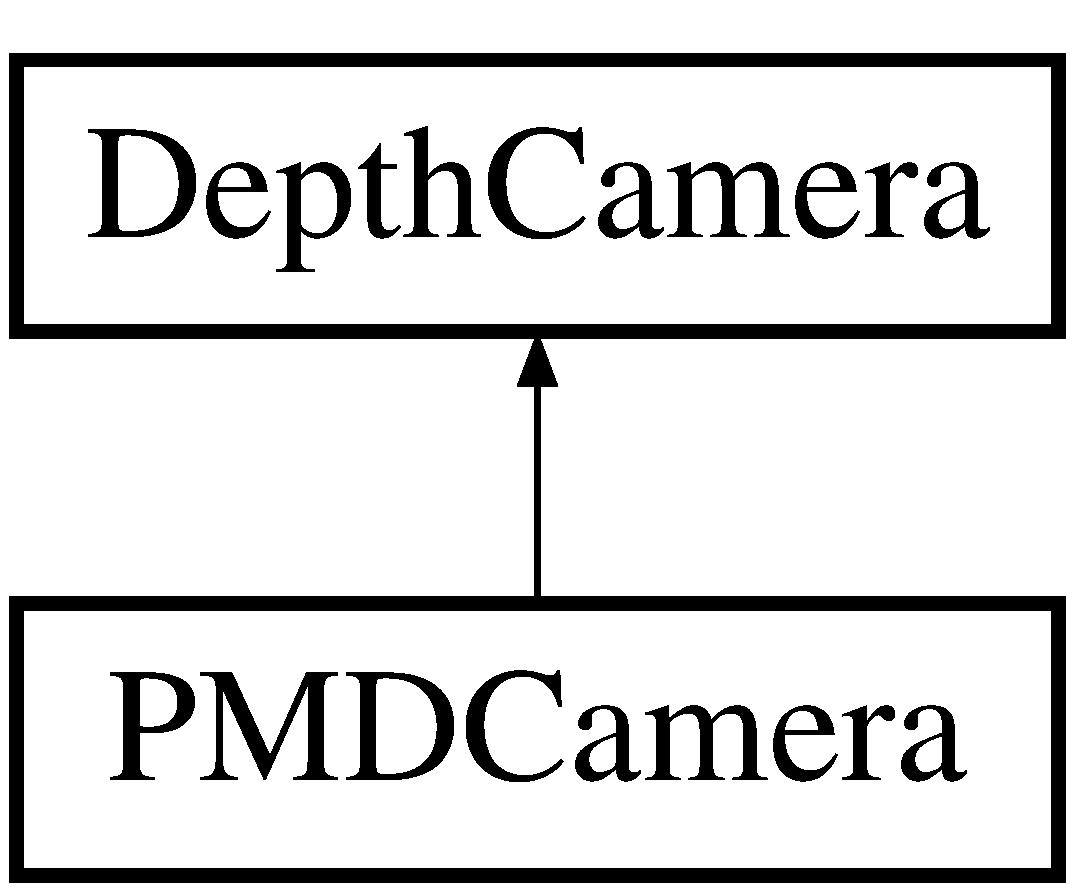
\includegraphics[height=2.000000cm]{class_p_m_d_camera}
\end{center}
\end{figure}
\subsection*{Public Member Functions}
\begin{DoxyCompactItemize}
\item 
\hyperlink{class_p_m_d_camera_a9965c089ec7eea8537e249d432c1dbba}{P\+M\+D\+Camera} (bool use\+\_\+live\+\_\+sensor=true)
\begin{DoxyCompactList}\small\item\em Public constructor initializing the P\+MD Camera. \end{DoxyCompactList}\item 
\hyperlink{class_p_m_d_camera_a645cc6c2b05896c776bfdde5bc1aa1f0}{$\sim$\+P\+M\+D\+Camera} ()
\begin{DoxyCompactList}\small\item\em Deconstructor for the P\+MD Camera. \end{DoxyCompactList}\item 
void \hyperlink{class_p_m_d_camera_aa6cb9398f9635436b4384ee2043def40}{update} ()
\begin{DoxyCompactList}\small\item\em Gets new frame from sensor. \end{DoxyCompactList}\item 
void \hyperlink{class_p_m_d_camera_a13090aeffb98e1440e715a93e67d3c0e}{destroy\+Instance} ()
\begin{DoxyCompactList}\small\item\em Gracefully closes the P\+MD camera. \end{DoxyCompactList}\end{DoxyCompactItemize}
\subsection*{Private Member Functions}
\begin{DoxyCompactItemize}
\item 
float \hyperlink{class_p_m_d_camera_a6d5662f8c84cb9c12ad71a70159a6f3a}{getX} (int i, int j) const
\begin{DoxyCompactList}\small\item\em Getter method for the x-\/coordinate at (i,j). \end{DoxyCompactList}\item 
float \hyperlink{class_p_m_d_camera_a71344967a964b6c45fc7dfd8b5f56e63}{getY} (int i, int j) const
\begin{DoxyCompactList}\small\item\em Getter method for the x-\/coordinate at (i,j). \end{DoxyCompactList}\item 
float \hyperlink{class_p_m_d_camera_a98254399959993d8a181f17402845457}{getZ} (int i, int j) const
\begin{DoxyCompactList}\small\item\em Getter method for the x-\/coordinate at (i,j). \end{DoxyCompactList}\item 
void \hyperlink{class_p_m_d_camera_a9d67405b9e1e4d4631b218adaa0326ed}{fill\+In\+Z\+Coords} ()
\begin{DoxyCompactList}\small\item\em Update the z-\/coordinates of the xyz\+Map. \end{DoxyCompactList}\item 
void \hyperlink{class_p_m_d_camera_aba055c818c275cf76d73527395937943}{fill\+In\+Amps} ()
\begin{DoxyCompactList}\small\item\em Update the values in the amp\+Map. \end{DoxyCompactList}\end{DoxyCompactItemize}
\subsection*{Private Attributes}
\begin{DoxyCompactItemize}
\item 
const char $\ast$ \hyperlink{class_p_m_d_camera_ae5c857a614ea51781c690fd862f0e7a2}{S\+O\+U\+R\+C\+E\+\_\+\+P\+L\+U\+G\+IN} = \char`\"{}camboardpico\char`\"{}
\item 
const char $\ast$ \hyperlink{class_p_m_d_camera_a439b2e8f27acbc26d4de70d9f8a82386}{S\+O\+U\+R\+C\+E\+\_\+\+P\+A\+R\+AM} = \char`\"{}\char`\"{}
\item 
const char $\ast$ \hyperlink{class_p_m_d_camera_a1f03b40bf2336e61879fc909490f2829}{P\+R\+O\+C\+\_\+\+P\+L\+U\+G\+IN} = \char`\"{}camboardpicoproc\char`\"{}
\item 
const char $\ast$ \hyperlink{class_p_m_d_camera_aef47cd1fda507e9921143f6d0302f5e0}{P\+R\+O\+C\+\_\+\+P\+A\+R\+AM} = \char`\"{}\char`\"{}
\item 
P\+M\+D\+Handle \hyperlink{class_p_m_d_camera_a4422b04aee07aed56b58847d39b2230f}{hnd}
\item 
P\+M\+D\+Data\+Description \hyperlink{class_p_m_d_camera_add31d3bba3f20568e45e3dd864a5bda9}{dd}
\item 
char \hyperlink{class_p_m_d_camera_a096946b5bca77dd8fe416c31f850ae75}{err} \mbox{[}128\mbox{]}
\item 
int \hyperlink{class_p_m_d_camera_a0c9627cf393f3055f81c7259c62010f6}{num\+Pixels}
\item 
float $\ast$ \hyperlink{class_p_m_d_camera_a6aa74776638ecb0b1869a1e12734870a}{dists}
\item 
float $\ast$ \hyperlink{class_p_m_d_camera_a315c2931504d25d5b5d882c4b2d9ad26}{amps}
\item 
Ipl\+Image $\ast$ \hyperlink{class_p_m_d_camera_ad47d6be8f7f11d2772690d3ea36dd432}{frame}
\item 
cv\+::\+Kalman\+Filter \hyperlink{class_p_m_d_camera_ad0d43501bb89e4f24f37e0ba5fa78ae6}{KF}
\item 
cv\+::\+Mat\+\_\+$<$ float $>$ \hyperlink{class_p_m_d_camera_ab7536178e056881c11756892c5f0a4b0}{measurement}
\end{DoxyCompactItemize}
\subsection*{Additional Inherited Members}


\subsection{Detailed Description}
Class defining the behavior of a P\+MD Camera. 

Example on how to read from sensor and visualize its output 
\begin{DoxyCodeInclude}
\textcolor{comment}{// C++ Libraries}
\textcolor{preprocessor}{#include <stdio.h>}
\textcolor{preprocessor}{#include <iostream>}
\textcolor{preprocessor}{#include <string>}

\textcolor{comment}{// OpenCV Libraries}
\textcolor{preprocessor}{#include <opencv/cxcore.h>}
\textcolor{preprocessor}{#include "opencv2/highgui/highgui.hpp"}

\textcolor{comment}{// OpenARK Libraries}
\textcolor{preprocessor}{#include "\hyperlink{_p_m_d_camera_8h}{PMDCamera.h}"}
\textcolor{preprocessor}{#include "\hyperlink{_visualizer_8h}{Visualizer.h}"}
\textcolor{preprocessor}{#include "\hyperlink{_util_8h}{Util.h}"}

\textcolor{keywordtype}{int} \hyperlink{main_8cpp_ae66f6b31b5ad750f1fe042a706a4e3d4}{main}() \{
    \hyperlink{class_depth_camera}{DepthCamera}* pmd = \textcolor{keyword}{new} \hyperlink{class_p_m_d_camera_a9965c089ec7eea8537e249d432c1dbba}{PMDCamera}();
    \textcolor{keywordtype}{int} frame = 0;
    
    \textcolor{keywordflow}{while} (\textcolor{keyword}{true})
    \{
        \textcolor{comment}{// Update the current frame}
        pmd->\hyperlink{class_depth_camera_abae1b9f37a00b17f00ff983ebb43ffc5}{update}();

        \textcolor{comment}{// REmove the current frame}
        pmd->\hyperlink{class_depth_camera_adc06db6509cc5f47de1e168f56bf41fa}{removeNoise}();

        \textcolor{comment}{// Visualize the XYZ Map}
        cv::imshow(\textcolor{stringliteral}{"XYZ Map"}, \hyperlink{class_visualizer_a24caf117be9878e2f5ad35cabb7f4f88}{Visualizer::visualizeXYZMap}(pmd->
      \hyperlink{class_depth_camera_a0c295c5a0696550f453b1c8cd0fcb188}{getXYZMap}()));
        
        \textcolor{comment}{/**** Start: Loop Break Condition ****/}
        \textcolor{keywordtype}{int} c = cvWaitKey(1);
        \textcolor{keywordflow}{if} (c == \textcolor{charliteral}{'q'} || c == \textcolor{charliteral}{'Q'} || c == 27) \{
            \textcolor{keywordflow}{break};
        \}
        \textcolor{comment}{/**** End: Loop Break Condition ****/}
        frame++;
    \}

    pmd->\hyperlink{class_depth_camera_aaf7c09a863e906f61104f23af10a8597}{destroyInstance}();
    \textcolor{keywordflow}{return} 0;
\}
\end{DoxyCodeInclude}
 

\subsection{Constructor \& Destructor Documentation}
\hypertarget{class_p_m_d_camera_a9965c089ec7eea8537e249d432c1dbba}{}\label{class_p_m_d_camera_a9965c089ec7eea8537e249d432c1dbba} 
\index{P\+M\+D\+Camera@{P\+M\+D\+Camera}!P\+M\+D\+Camera@{P\+M\+D\+Camera}}
\index{P\+M\+D\+Camera@{P\+M\+D\+Camera}!P\+M\+D\+Camera@{P\+M\+D\+Camera}}
\subsubsection{\texorpdfstring{P\+M\+D\+Camera()}{PMDCamera()}}
{\footnotesize\ttfamily P\+M\+D\+Camera\+::\+P\+M\+D\+Camera (\begin{DoxyParamCaption}\item[{bool}]{use\+\_\+live\+\_\+sensor = {\ttfamily true} }\end{DoxyParamCaption})}



Public constructor initializing the P\+MD Camera. 


\begin{DoxyParams}{Parameters}
{\em use\+\_\+live\+\_\+sensor} & uses input from real sensor if T\+R\+UE. Otherwise reads from input file. Default is set to T\+R\+UE. \\
\hline
\end{DoxyParams}
\hypertarget{class_p_m_d_camera_a645cc6c2b05896c776bfdde5bc1aa1f0}{}\label{class_p_m_d_camera_a645cc6c2b05896c776bfdde5bc1aa1f0} 
\index{P\+M\+D\+Camera@{P\+M\+D\+Camera}!````~P\+M\+D\+Camera@{$\sim$\+P\+M\+D\+Camera}}
\index{````~P\+M\+D\+Camera@{$\sim$\+P\+M\+D\+Camera}!P\+M\+D\+Camera@{P\+M\+D\+Camera}}
\subsubsection{\texorpdfstring{$\sim$\+P\+M\+D\+Camera()}{~PMDCamera()}}
{\footnotesize\ttfamily P\+M\+D\+Camera\+::$\sim$\+P\+M\+D\+Camera (\begin{DoxyParamCaption}{ }\end{DoxyParamCaption})}



Deconstructor for the P\+MD Camera. 



\subsection{Member Function Documentation}
\hypertarget{class_p_m_d_camera_a13090aeffb98e1440e715a93e67d3c0e}{}\label{class_p_m_d_camera_a13090aeffb98e1440e715a93e67d3c0e} 
\index{P\+M\+D\+Camera@{P\+M\+D\+Camera}!destroy\+Instance@{destroy\+Instance}}
\index{destroy\+Instance@{destroy\+Instance}!P\+M\+D\+Camera@{P\+M\+D\+Camera}}
\subsubsection{\texorpdfstring{destroy\+Instance()}{destroyInstance()}}
{\footnotesize\ttfamily void P\+M\+D\+Camera\+::destroy\+Instance (\begin{DoxyParamCaption}{ }\end{DoxyParamCaption})\hspace{0.3cm}{\ttfamily [virtual]}}



Gracefully closes the P\+MD camera. 



Implements \hyperlink{class_depth_camera_aaf7c09a863e906f61104f23af10a8597}{Depth\+Camera}.

\hypertarget{class_p_m_d_camera_aba055c818c275cf76d73527395937943}{}\label{class_p_m_d_camera_aba055c818c275cf76d73527395937943} 
\index{P\+M\+D\+Camera@{P\+M\+D\+Camera}!fill\+In\+Amps@{fill\+In\+Amps}}
\index{fill\+In\+Amps@{fill\+In\+Amps}!P\+M\+D\+Camera@{P\+M\+D\+Camera}}
\subsubsection{\texorpdfstring{fill\+In\+Amps()}{fillInAmps()}}
{\footnotesize\ttfamily void P\+M\+D\+Camera\+::fill\+In\+Amps (\begin{DoxyParamCaption}{ }\end{DoxyParamCaption})\hspace{0.3cm}{\ttfamily [private]}}



Update the values in the amp\+Map. 

\hypertarget{class_p_m_d_camera_a9d67405b9e1e4d4631b218adaa0326ed}{}\label{class_p_m_d_camera_a9d67405b9e1e4d4631b218adaa0326ed} 
\index{P\+M\+D\+Camera@{P\+M\+D\+Camera}!fill\+In\+Z\+Coords@{fill\+In\+Z\+Coords}}
\index{fill\+In\+Z\+Coords@{fill\+In\+Z\+Coords}!P\+M\+D\+Camera@{P\+M\+D\+Camera}}
\subsubsection{\texorpdfstring{fill\+In\+Z\+Coords()}{fillInZCoords()}}
{\footnotesize\ttfamily void P\+M\+D\+Camera\+::fill\+In\+Z\+Coords (\begin{DoxyParamCaption}{ }\end{DoxyParamCaption})\hspace{0.3cm}{\ttfamily [private]}}



Update the z-\/coordinates of the xyz\+Map. 

\hypertarget{class_p_m_d_camera_a6d5662f8c84cb9c12ad71a70159a6f3a}{}\label{class_p_m_d_camera_a6d5662f8c84cb9c12ad71a70159a6f3a} 
\index{P\+M\+D\+Camera@{P\+M\+D\+Camera}!getX@{getX}}
\index{getX@{getX}!P\+M\+D\+Camera@{P\+M\+D\+Camera}}
\subsubsection{\texorpdfstring{get\+X()}{getX()}}
{\footnotesize\ttfamily float P\+M\+D\+Camera\+::getX (\begin{DoxyParamCaption}\item[{int}]{i,  }\item[{int}]{j }\end{DoxyParamCaption}) const\hspace{0.3cm}{\ttfamily [private]}}



Getter method for the x-\/coordinate at (i,j). 


\begin{DoxyParams}{Parameters}
{\em i} & ith row \\
\hline
{\em j} & jth column \\
\hline
\end{DoxyParams}
\begin{DoxyReturn}{Returns}
x-\/coodinate at (i,j) 
\end{DoxyReturn}
\hypertarget{class_p_m_d_camera_a71344967a964b6c45fc7dfd8b5f56e63}{}\label{class_p_m_d_camera_a71344967a964b6c45fc7dfd8b5f56e63} 
\index{P\+M\+D\+Camera@{P\+M\+D\+Camera}!getY@{getY}}
\index{getY@{getY}!P\+M\+D\+Camera@{P\+M\+D\+Camera}}
\subsubsection{\texorpdfstring{get\+Y()}{getY()}}
{\footnotesize\ttfamily float P\+M\+D\+Camera\+::getY (\begin{DoxyParamCaption}\item[{int}]{i,  }\item[{int}]{j }\end{DoxyParamCaption}) const\hspace{0.3cm}{\ttfamily [private]}}



Getter method for the x-\/coordinate at (i,j). 


\begin{DoxyParams}{Parameters}
{\em i} & ith row \\
\hline
{\em j} & jth column \\
\hline
\end{DoxyParams}
\begin{DoxyReturn}{Returns}
x-\/coodinate at (i,j) 
\end{DoxyReturn}
\hypertarget{class_p_m_d_camera_a98254399959993d8a181f17402845457}{}\label{class_p_m_d_camera_a98254399959993d8a181f17402845457} 
\index{P\+M\+D\+Camera@{P\+M\+D\+Camera}!getZ@{getZ}}
\index{getZ@{getZ}!P\+M\+D\+Camera@{P\+M\+D\+Camera}}
\subsubsection{\texorpdfstring{get\+Z()}{getZ()}}
{\footnotesize\ttfamily float P\+M\+D\+Camera\+::getZ (\begin{DoxyParamCaption}\item[{int}]{i,  }\item[{int}]{j }\end{DoxyParamCaption}) const\hspace{0.3cm}{\ttfamily [private]}}



Getter method for the x-\/coordinate at (i,j). 


\begin{DoxyParams}{Parameters}
{\em i} & ith row \\
\hline
{\em j} & jth column \\
\hline
\end{DoxyParams}
\begin{DoxyReturn}{Returns}
x-\/coodinate at (i,j) 
\end{DoxyReturn}
\hypertarget{class_p_m_d_camera_aa6cb9398f9635436b4384ee2043def40}{}\label{class_p_m_d_camera_aa6cb9398f9635436b4384ee2043def40} 
\index{P\+M\+D\+Camera@{P\+M\+D\+Camera}!update@{update}}
\index{update@{update}!P\+M\+D\+Camera@{P\+M\+D\+Camera}}
\subsubsection{\texorpdfstring{update()}{update()}}
{\footnotesize\ttfamily void P\+M\+D\+Camera\+::update (\begin{DoxyParamCaption}{ }\end{DoxyParamCaption})\hspace{0.3cm}{\ttfamily [virtual]}}



Gets new frame from sensor. 

Updates xyz\+Map, amp\+Map, and flag\+Map. Resets clusters. 

Implements \hyperlink{class_depth_camera_abae1b9f37a00b17f00ff983ebb43ffc5}{Depth\+Camera}.



\subsection{Member Data Documentation}
\hypertarget{class_p_m_d_camera_a315c2931504d25d5b5d882c4b2d9ad26}{}\label{class_p_m_d_camera_a315c2931504d25d5b5d882c4b2d9ad26} 
\index{P\+M\+D\+Camera@{P\+M\+D\+Camera}!amps@{amps}}
\index{amps@{amps}!P\+M\+D\+Camera@{P\+M\+D\+Camera}}
\subsubsection{\texorpdfstring{amps}{amps}}
{\footnotesize\ttfamily float$\ast$ P\+M\+D\+Camera\+::amps\hspace{0.3cm}{\ttfamily [private]}}

\hypertarget{class_p_m_d_camera_add31d3bba3f20568e45e3dd864a5bda9}{}\label{class_p_m_d_camera_add31d3bba3f20568e45e3dd864a5bda9} 
\index{P\+M\+D\+Camera@{P\+M\+D\+Camera}!dd@{dd}}
\index{dd@{dd}!P\+M\+D\+Camera@{P\+M\+D\+Camera}}
\subsubsection{\texorpdfstring{dd}{dd}}
{\footnotesize\ttfamily P\+M\+D\+Data\+Description P\+M\+D\+Camera\+::dd\hspace{0.3cm}{\ttfamily [private]}}

\hypertarget{class_p_m_d_camera_a6aa74776638ecb0b1869a1e12734870a}{}\label{class_p_m_d_camera_a6aa74776638ecb0b1869a1e12734870a} 
\index{P\+M\+D\+Camera@{P\+M\+D\+Camera}!dists@{dists}}
\index{dists@{dists}!P\+M\+D\+Camera@{P\+M\+D\+Camera}}
\subsubsection{\texorpdfstring{dists}{dists}}
{\footnotesize\ttfamily float$\ast$ P\+M\+D\+Camera\+::dists\hspace{0.3cm}{\ttfamily [private]}}

\hypertarget{class_p_m_d_camera_a096946b5bca77dd8fe416c31f850ae75}{}\label{class_p_m_d_camera_a096946b5bca77dd8fe416c31f850ae75} 
\index{P\+M\+D\+Camera@{P\+M\+D\+Camera}!err@{err}}
\index{err@{err}!P\+M\+D\+Camera@{P\+M\+D\+Camera}}
\subsubsection{\texorpdfstring{err}{err}}
{\footnotesize\ttfamily char P\+M\+D\+Camera\+::err\mbox{[}128\mbox{]}\hspace{0.3cm}{\ttfamily [private]}}

\hypertarget{class_p_m_d_camera_ad47d6be8f7f11d2772690d3ea36dd432}{}\label{class_p_m_d_camera_ad47d6be8f7f11d2772690d3ea36dd432} 
\index{P\+M\+D\+Camera@{P\+M\+D\+Camera}!frame@{frame}}
\index{frame@{frame}!P\+M\+D\+Camera@{P\+M\+D\+Camera}}
\subsubsection{\texorpdfstring{frame}{frame}}
{\footnotesize\ttfamily Ipl\+Image$\ast$ P\+M\+D\+Camera\+::frame\hspace{0.3cm}{\ttfamily [private]}}

\hypertarget{class_p_m_d_camera_a4422b04aee07aed56b58847d39b2230f}{}\label{class_p_m_d_camera_a4422b04aee07aed56b58847d39b2230f} 
\index{P\+M\+D\+Camera@{P\+M\+D\+Camera}!hnd@{hnd}}
\index{hnd@{hnd}!P\+M\+D\+Camera@{P\+M\+D\+Camera}}
\subsubsection{\texorpdfstring{hnd}{hnd}}
{\footnotesize\ttfamily P\+M\+D\+Handle P\+M\+D\+Camera\+::hnd\hspace{0.3cm}{\ttfamily [private]}}

\hypertarget{class_p_m_d_camera_ad0d43501bb89e4f24f37e0ba5fa78ae6}{}\label{class_p_m_d_camera_ad0d43501bb89e4f24f37e0ba5fa78ae6} 
\index{P\+M\+D\+Camera@{P\+M\+D\+Camera}!KF@{KF}}
\index{KF@{KF}!P\+M\+D\+Camera@{P\+M\+D\+Camera}}
\subsubsection{\texorpdfstring{KF}{KF}}
{\footnotesize\ttfamily cv\+::\+Kalman\+Filter P\+M\+D\+Camera\+::\+KF\hspace{0.3cm}{\ttfamily [private]}}

\hypertarget{class_p_m_d_camera_ab7536178e056881c11756892c5f0a4b0}{}\label{class_p_m_d_camera_ab7536178e056881c11756892c5f0a4b0} 
\index{P\+M\+D\+Camera@{P\+M\+D\+Camera}!measurement@{measurement}}
\index{measurement@{measurement}!P\+M\+D\+Camera@{P\+M\+D\+Camera}}
\subsubsection{\texorpdfstring{measurement}{measurement}}
{\footnotesize\ttfamily cv\+::\+Mat\+\_\+$<$float$>$ P\+M\+D\+Camera\+::measurement\hspace{0.3cm}{\ttfamily [private]}}

\hypertarget{class_p_m_d_camera_a0c9627cf393f3055f81c7259c62010f6}{}\label{class_p_m_d_camera_a0c9627cf393f3055f81c7259c62010f6} 
\index{P\+M\+D\+Camera@{P\+M\+D\+Camera}!num\+Pixels@{num\+Pixels}}
\index{num\+Pixels@{num\+Pixels}!P\+M\+D\+Camera@{P\+M\+D\+Camera}}
\subsubsection{\texorpdfstring{num\+Pixels}{numPixels}}
{\footnotesize\ttfamily int P\+M\+D\+Camera\+::num\+Pixels\hspace{0.3cm}{\ttfamily [private]}}

\hypertarget{class_p_m_d_camera_aef47cd1fda507e9921143f6d0302f5e0}{}\label{class_p_m_d_camera_aef47cd1fda507e9921143f6d0302f5e0} 
\index{P\+M\+D\+Camera@{P\+M\+D\+Camera}!P\+R\+O\+C\+\_\+\+P\+A\+R\+AM@{P\+R\+O\+C\+\_\+\+P\+A\+R\+AM}}
\index{P\+R\+O\+C\+\_\+\+P\+A\+R\+AM@{P\+R\+O\+C\+\_\+\+P\+A\+R\+AM}!P\+M\+D\+Camera@{P\+M\+D\+Camera}}
\subsubsection{\texorpdfstring{P\+R\+O\+C\+\_\+\+P\+A\+R\+AM}{PROC\_PARAM}}
{\footnotesize\ttfamily const char$\ast$ P\+M\+D\+Camera\+::\+P\+R\+O\+C\+\_\+\+P\+A\+R\+AM = \char`\"{}\char`\"{}\hspace{0.3cm}{\ttfamily [private]}}

\hypertarget{class_p_m_d_camera_a1f03b40bf2336e61879fc909490f2829}{}\label{class_p_m_d_camera_a1f03b40bf2336e61879fc909490f2829} 
\index{P\+M\+D\+Camera@{P\+M\+D\+Camera}!P\+R\+O\+C\+\_\+\+P\+L\+U\+G\+IN@{P\+R\+O\+C\+\_\+\+P\+L\+U\+G\+IN}}
\index{P\+R\+O\+C\+\_\+\+P\+L\+U\+G\+IN@{P\+R\+O\+C\+\_\+\+P\+L\+U\+G\+IN}!P\+M\+D\+Camera@{P\+M\+D\+Camera}}
\subsubsection{\texorpdfstring{P\+R\+O\+C\+\_\+\+P\+L\+U\+G\+IN}{PROC\_PLUGIN}}
{\footnotesize\ttfamily const char$\ast$ P\+M\+D\+Camera\+::\+P\+R\+O\+C\+\_\+\+P\+L\+U\+G\+IN = \char`\"{}camboardpicoproc\char`\"{}\hspace{0.3cm}{\ttfamily [private]}}

\hypertarget{class_p_m_d_camera_a439b2e8f27acbc26d4de70d9f8a82386}{}\label{class_p_m_d_camera_a439b2e8f27acbc26d4de70d9f8a82386} 
\index{P\+M\+D\+Camera@{P\+M\+D\+Camera}!S\+O\+U\+R\+C\+E\+\_\+\+P\+A\+R\+AM@{S\+O\+U\+R\+C\+E\+\_\+\+P\+A\+R\+AM}}
\index{S\+O\+U\+R\+C\+E\+\_\+\+P\+A\+R\+AM@{S\+O\+U\+R\+C\+E\+\_\+\+P\+A\+R\+AM}!P\+M\+D\+Camera@{P\+M\+D\+Camera}}
\subsubsection{\texorpdfstring{S\+O\+U\+R\+C\+E\+\_\+\+P\+A\+R\+AM}{SOURCE\_PARAM}}
{\footnotesize\ttfamily const char$\ast$ P\+M\+D\+Camera\+::\+S\+O\+U\+R\+C\+E\+\_\+\+P\+A\+R\+AM = \char`\"{}\char`\"{}\hspace{0.3cm}{\ttfamily [private]}}

\hypertarget{class_p_m_d_camera_ae5c857a614ea51781c690fd862f0e7a2}{}\label{class_p_m_d_camera_ae5c857a614ea51781c690fd862f0e7a2} 
\index{P\+M\+D\+Camera@{P\+M\+D\+Camera}!S\+O\+U\+R\+C\+E\+\_\+\+P\+L\+U\+G\+IN@{S\+O\+U\+R\+C\+E\+\_\+\+P\+L\+U\+G\+IN}}
\index{S\+O\+U\+R\+C\+E\+\_\+\+P\+L\+U\+G\+IN@{S\+O\+U\+R\+C\+E\+\_\+\+P\+L\+U\+G\+IN}!P\+M\+D\+Camera@{P\+M\+D\+Camera}}
\subsubsection{\texorpdfstring{S\+O\+U\+R\+C\+E\+\_\+\+P\+L\+U\+G\+IN}{SOURCE\_PLUGIN}}
{\footnotesize\ttfamily const char$\ast$ P\+M\+D\+Camera\+::\+S\+O\+U\+R\+C\+E\+\_\+\+P\+L\+U\+G\+IN = \char`\"{}camboardpico\char`\"{}\hspace{0.3cm}{\ttfamily [private]}}



The documentation for this class was generated from the following files\+:\begin{DoxyCompactItemize}
\item 
\hyperlink{_p_m_d_camera_8h}{P\+M\+D\+Camera.\+h}\item 
\hyperlink{_p_m_d_camera_8cpp}{P\+M\+D\+Camera.\+cpp}\end{DoxyCompactItemize}

\hypertarget{class_r_g_b_camera}{}\section{R\+G\+B\+Camera Class Reference}
\label{class_r_g_b_camera}\index{R\+G\+B\+Camera@{R\+G\+B\+Camera}}


Abstract class that defines the behavior of a R\+GB camera.  




{\ttfamily \#include $<$R\+G\+B\+Camera.\+h$>$}

Inheritance diagram for R\+G\+B\+Camera\+:\begin{figure}[H]
\begin{center}
\leavevmode
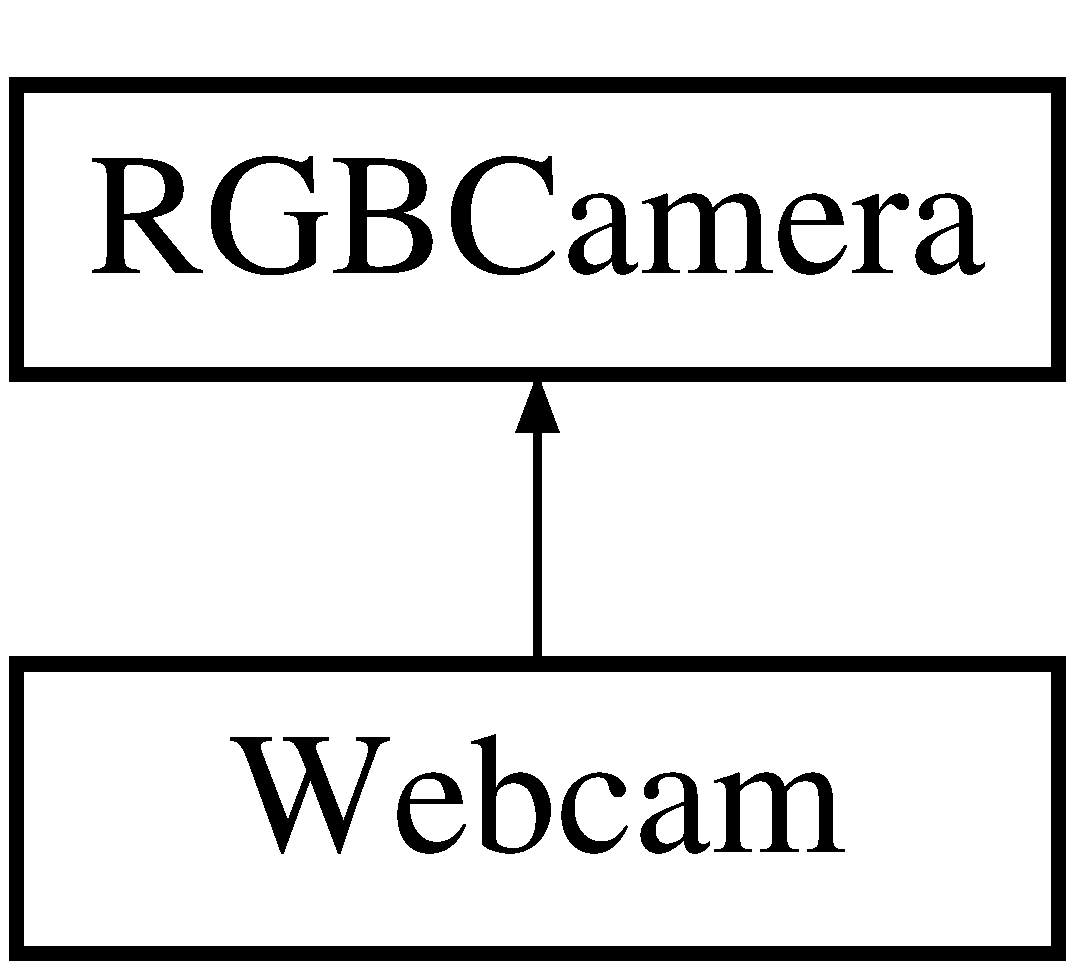
\includegraphics[height=2.000000cm]{class_r_g_b_camera}
\end{center}
\end{figure}
\subsection*{Public Member Functions}
\begin{DoxyCompactItemize}
\item 
virtual void \hyperlink{class_r_g_b_camera_ac9fa3f8f32605e846827b694ae7cff18}{update} ()=0
\begin{DoxyCompactList}\small\item\em Updates the current frame on the R\+GB camera. \end{DoxyCompactList}\item 
cv\+::\+Mat \hyperlink{class_r_g_b_camera_a4db0620e9346039530f248fbb7130212}{get\+Frame} ()
\begin{DoxyCompactList}\small\item\em Returns the current frame. \end{DoxyCompactList}\end{DoxyCompactItemize}
\subsection*{Protected Attributes}
\begin{DoxyCompactItemize}
\item 
cv\+::\+Video\+Capture \hyperlink{class_r_g_b_camera_a941480d7209fdae8f0ac410cb6b90a63}{cap}
\begin{DoxyCompactList}\small\item\em Camera handle. \end{DoxyCompactList}\item 
cv\+::\+Mat \hyperlink{class_r_g_b_camera_a81487c499dd5eee3c573ec6ed721ceba}{frame}
\begin{DoxyCompactList}\small\item\em Current frame. \end{DoxyCompactList}\end{DoxyCompactItemize}


\subsection{Detailed Description}
Abstract class that defines the behavior of a R\+GB camera. 

\subsection{Member Function Documentation}
\hypertarget{class_r_g_b_camera_a4db0620e9346039530f248fbb7130212}{}\label{class_r_g_b_camera_a4db0620e9346039530f248fbb7130212} 
\index{R\+G\+B\+Camera@{R\+G\+B\+Camera}!get\+Frame@{get\+Frame}}
\index{get\+Frame@{get\+Frame}!R\+G\+B\+Camera@{R\+G\+B\+Camera}}
\subsubsection{\texorpdfstring{get\+Frame()}{getFrame()}}
{\footnotesize\ttfamily cv\+::\+Mat R\+G\+B\+Camera\+::get\+Frame (\begin{DoxyParamCaption}{ }\end{DoxyParamCaption})}



Returns the current frame. 

\begin{DoxyReturn}{Returns}
the current frame 
\end{DoxyReturn}
\hypertarget{class_r_g_b_camera_ac9fa3f8f32605e846827b694ae7cff18}{}\label{class_r_g_b_camera_ac9fa3f8f32605e846827b694ae7cff18} 
\index{R\+G\+B\+Camera@{R\+G\+B\+Camera}!update@{update}}
\index{update@{update}!R\+G\+B\+Camera@{R\+G\+B\+Camera}}
\subsubsection{\texorpdfstring{update()}{update()}}
{\footnotesize\ttfamily virtual void R\+G\+B\+Camera\+::update (\begin{DoxyParamCaption}{ }\end{DoxyParamCaption})\hspace{0.3cm}{\ttfamily [pure virtual]}}



Updates the current frame on the R\+GB camera. 

Should be overriden by a concerte implementation specific to the R\+GB camera 

Implemented in \hyperlink{class_webcam_a3d5cab0a2b87b90b85793bc05414e503}{Webcam}.



\subsection{Member Data Documentation}
\hypertarget{class_r_g_b_camera_a941480d7209fdae8f0ac410cb6b90a63}{}\label{class_r_g_b_camera_a941480d7209fdae8f0ac410cb6b90a63} 
\index{R\+G\+B\+Camera@{R\+G\+B\+Camera}!cap@{cap}}
\index{cap@{cap}!R\+G\+B\+Camera@{R\+G\+B\+Camera}}
\subsubsection{\texorpdfstring{cap}{cap}}
{\footnotesize\ttfamily cv\+::\+Video\+Capture R\+G\+B\+Camera\+::cap\hspace{0.3cm}{\ttfamily [protected]}}



Camera handle. 

\hypertarget{class_r_g_b_camera_a81487c499dd5eee3c573ec6ed721ceba}{}\label{class_r_g_b_camera_a81487c499dd5eee3c573ec6ed721ceba} 
\index{R\+G\+B\+Camera@{R\+G\+B\+Camera}!frame@{frame}}
\index{frame@{frame}!R\+G\+B\+Camera@{R\+G\+B\+Camera}}
\subsubsection{\texorpdfstring{frame}{frame}}
{\footnotesize\ttfamily cv\+::\+Mat R\+G\+B\+Camera\+::frame\hspace{0.3cm}{\ttfamily [protected]}}



Current frame. 



The documentation for this class was generated from the following files\+:\begin{DoxyCompactItemize}
\item 
\hyperlink{_r_g_b_camera_8h}{R\+G\+B\+Camera.\+h}\item 
\hyperlink{_r_g_b_camera_8cpp}{R\+G\+B\+Camera.\+cpp}\end{DoxyCompactItemize}

\hypertarget{class_u_d_p_sender}{}\section{U\+D\+P\+Sender Class Reference}
\label{class_u_d_p_sender}\index{U\+D\+P\+Sender@{U\+D\+P\+Sender}}


U\+DP client.  




{\ttfamily \#include $<$U\+D\+P\+Sender.\+h$>$}

\subsection*{Public Member Functions}
\begin{DoxyCompactItemize}
\item 
\hyperlink{class_u_d_p_sender_a77c0f2eb66dbc9a912b4fede20de3f03}{U\+D\+P\+Sender} ()
\begin{DoxyCompactList}\small\item\em Constructs a new U\+PD sender. \end{DoxyCompactList}\item 
int \hyperlink{class_u_d_p_sender_a33d402a42a2d512bd12189e1f698cca4}{send} (std\+::string \hyperlink{class_u_d_p_sender_a738a29b72c2c7fe5655e74cd4ee0e077}{message})
\begin{DoxyCompactList}\small\item\em Sends a message. \end{DoxyCompactList}\item 
int \hyperlink{class_u_d_p_sender_a9633801c0b923a53d42061f2233d06ef}{close} ()
\begin{DoxyCompactList}\small\item\em Close the current connection. \end{DoxyCompactList}\end{DoxyCompactItemize}
\subsection*{Public Attributes}
\begin{DoxyCompactItemize}
\item 
struct sockaddr\+\_\+in \hyperlink{class_u_d_p_sender_abeda008425d14ea8092d23d23bbd1117}{si\+\_\+other}
\item 
int \hyperlink{class_u_d_p_sender_aeb3773ffb3bc9549dbe73c0e7fee0f23}{s}
\item 
int \hyperlink{class_u_d_p_sender_a44e4545b002409e774edb7e30653d53e}{slen} = sizeof(\hyperlink{class_u_d_p_sender_abeda008425d14ea8092d23d23bbd1117}{si\+\_\+other})
\item 
char \hyperlink{class_u_d_p_sender_a21073b873007a83ac5bec30bcce8fd43}{buf} \mbox{[}\hyperlink{_u_d_p_sender_8h_ad974fe981249f5e84fbf1683b012c9f8}{B\+U\+F\+L\+EN}\mbox{]}
\item 
char \hyperlink{class_u_d_p_sender_a738a29b72c2c7fe5655e74cd4ee0e077}{message} \mbox{[}\hyperlink{_u_d_p_sender_8h_ad974fe981249f5e84fbf1683b012c9f8}{B\+U\+F\+L\+EN}\mbox{]}
\item 
W\+S\+A\+D\+A\+TA \hyperlink{class_u_d_p_sender_afc9fc0d12ba056af8f66ee738c5bbe98}{wsa}
\end{DoxyCompactItemize}


\subsection{Detailed Description}
U\+DP client. 

Used to communicate information with game engines such as Unity 

\subsection{Constructor \& Destructor Documentation}
\hypertarget{class_u_d_p_sender_a77c0f2eb66dbc9a912b4fede20de3f03}{}\label{class_u_d_p_sender_a77c0f2eb66dbc9a912b4fede20de3f03} 
\index{U\+D\+P\+Sender@{U\+D\+P\+Sender}!U\+D\+P\+Sender@{U\+D\+P\+Sender}}
\index{U\+D\+P\+Sender@{U\+D\+P\+Sender}!U\+D\+P\+Sender@{U\+D\+P\+Sender}}
\subsubsection{\texorpdfstring{U\+D\+P\+Sender()}{UDPSender()}}
{\footnotesize\ttfamily U\+D\+P\+Sender\+::\+U\+D\+P\+Sender (\begin{DoxyParamCaption}{ }\end{DoxyParamCaption})}



Constructs a new U\+PD sender. 



\subsection{Member Function Documentation}
\hypertarget{class_u_d_p_sender_a9633801c0b923a53d42061f2233d06ef}{}\label{class_u_d_p_sender_a9633801c0b923a53d42061f2233d06ef} 
\index{U\+D\+P\+Sender@{U\+D\+P\+Sender}!close@{close}}
\index{close@{close}!U\+D\+P\+Sender@{U\+D\+P\+Sender}}
\subsubsection{\texorpdfstring{close()}{close()}}
{\footnotesize\ttfamily int U\+D\+P\+Sender\+::close (\begin{DoxyParamCaption}{ }\end{DoxyParamCaption})}



Close the current connection. 

\hypertarget{class_u_d_p_sender_a33d402a42a2d512bd12189e1f698cca4}{}\label{class_u_d_p_sender_a33d402a42a2d512bd12189e1f698cca4} 
\index{U\+D\+P\+Sender@{U\+D\+P\+Sender}!send@{send}}
\index{send@{send}!U\+D\+P\+Sender@{U\+D\+P\+Sender}}
\subsubsection{\texorpdfstring{send()}{send()}}
{\footnotesize\ttfamily int U\+D\+P\+Sender\+::send (\begin{DoxyParamCaption}\item[{std\+::string}]{message }\end{DoxyParamCaption})}



Sends a message. 


\begin{DoxyParams}{Parameters}
{\em message} & the data to be sent \\
\hline
\end{DoxyParams}


\subsection{Member Data Documentation}
\hypertarget{class_u_d_p_sender_a21073b873007a83ac5bec30bcce8fd43}{}\label{class_u_d_p_sender_a21073b873007a83ac5bec30bcce8fd43} 
\index{U\+D\+P\+Sender@{U\+D\+P\+Sender}!buf@{buf}}
\index{buf@{buf}!U\+D\+P\+Sender@{U\+D\+P\+Sender}}
\subsubsection{\texorpdfstring{buf}{buf}}
{\footnotesize\ttfamily char U\+D\+P\+Sender\+::buf\mbox{[}\hyperlink{_u_d_p_sender_8h_ad974fe981249f5e84fbf1683b012c9f8}{B\+U\+F\+L\+EN}\mbox{]}}

\hypertarget{class_u_d_p_sender_a738a29b72c2c7fe5655e74cd4ee0e077}{}\label{class_u_d_p_sender_a738a29b72c2c7fe5655e74cd4ee0e077} 
\index{U\+D\+P\+Sender@{U\+D\+P\+Sender}!message@{message}}
\index{message@{message}!U\+D\+P\+Sender@{U\+D\+P\+Sender}}
\subsubsection{\texorpdfstring{message}{message}}
{\footnotesize\ttfamily char U\+D\+P\+Sender\+::message\mbox{[}\hyperlink{_u_d_p_sender_8h_ad974fe981249f5e84fbf1683b012c9f8}{B\+U\+F\+L\+EN}\mbox{]}}

\hypertarget{class_u_d_p_sender_aeb3773ffb3bc9549dbe73c0e7fee0f23}{}\label{class_u_d_p_sender_aeb3773ffb3bc9549dbe73c0e7fee0f23} 
\index{U\+D\+P\+Sender@{U\+D\+P\+Sender}!s@{s}}
\index{s@{s}!U\+D\+P\+Sender@{U\+D\+P\+Sender}}
\subsubsection{\texorpdfstring{s}{s}}
{\footnotesize\ttfamily int U\+D\+P\+Sender\+::s}

\hypertarget{class_u_d_p_sender_abeda008425d14ea8092d23d23bbd1117}{}\label{class_u_d_p_sender_abeda008425d14ea8092d23d23bbd1117} 
\index{U\+D\+P\+Sender@{U\+D\+P\+Sender}!si\+\_\+other@{si\+\_\+other}}
\index{si\+\_\+other@{si\+\_\+other}!U\+D\+P\+Sender@{U\+D\+P\+Sender}}
\subsubsection{\texorpdfstring{si\+\_\+other}{si\_other}}
{\footnotesize\ttfamily struct sockaddr\+\_\+in U\+D\+P\+Sender\+::si\+\_\+other}

\hypertarget{class_u_d_p_sender_a44e4545b002409e774edb7e30653d53e}{}\label{class_u_d_p_sender_a44e4545b002409e774edb7e30653d53e} 
\index{U\+D\+P\+Sender@{U\+D\+P\+Sender}!slen@{slen}}
\index{slen@{slen}!U\+D\+P\+Sender@{U\+D\+P\+Sender}}
\subsubsection{\texorpdfstring{slen}{slen}}
{\footnotesize\ttfamily int U\+D\+P\+Sender\+::slen = sizeof(\hyperlink{class_u_d_p_sender_abeda008425d14ea8092d23d23bbd1117}{si\+\_\+other})}

\hypertarget{class_u_d_p_sender_afc9fc0d12ba056af8f66ee738c5bbe98}{}\label{class_u_d_p_sender_afc9fc0d12ba056af8f66ee738c5bbe98} 
\index{U\+D\+P\+Sender@{U\+D\+P\+Sender}!wsa@{wsa}}
\index{wsa@{wsa}!U\+D\+P\+Sender@{U\+D\+P\+Sender}}
\subsubsection{\texorpdfstring{wsa}{wsa}}
{\footnotesize\ttfamily W\+S\+A\+D\+A\+TA U\+D\+P\+Sender\+::wsa}



The documentation for this class was generated from the following files\+:\begin{DoxyCompactItemize}
\item 
\hyperlink{_u_d_p_sender_8h}{U\+D\+P\+Sender.\+h}\item 
\hyperlink{_u_d_p_sender_8cpp}{U\+D\+P\+Sender.\+cpp}\end{DoxyCompactItemize}

\hypertarget{class_util}{}\section{Util Class Reference}
\label{class_util}\index{Util@{Util}}


Class containing generic helper functions.  




{\ttfamily \#include $<$Util.\+h$>$}

\subsection*{Static Public Member Functions}
\begin{DoxyCompactItemize}
\item 
static cv\+::\+Vec3b \hyperlink{class_util_a4b35aebe2f6ea734a9221356c0ad38ec}{color\+Generator2} ()
\begin{DoxyCompactList}\small\item\em Generates a random R\+GB color. \end{DoxyCompactList}\item 
static int \hyperlink{class_util_a1213364e3ea975aa7f3713f3ad5a96a7}{get\+DistanceT} (int x1, int y1, int x2, int y2)
\begin{DoxyCompactList}\small\item\em Get euclidean distance between two 2D points. \end{DoxyCompactList}\item 
static float \hyperlink{class_util_a003878685d2eba96fadc4fdae502688e}{normalize} (float a, float b)
\begin{DoxyCompactList}\small\item\em Return the hypotenuse length. \end{DoxyCompactList}\item 
static double \hyperlink{class_util_afcaa0a0b92e0fd117be8dead6a7787f3}{euclidian\+Distance3D} (cv\+::\+Vec3f pt1, cv\+::\+Vec3f pt2)
\begin{DoxyCompactList}\small\item\em Get euclidean distance between two 3D points. \end{DoxyCompactList}\item 
static cv\+::\+Mat \hyperlink{class_util_abf2cc717b8e145166f247df2742a0325}{remove\+Points} (cv\+::\+Mat img, std\+::vector$<$ cv\+::\+Point2i $>$ points)
\begin{DoxyCompactList}\small\item\em Removes points on img with indicies defined in points. \end{DoxyCompactList}\item 
static cv\+::\+Vec3f \hyperlink{class_util_ab6f41d0184eb52fb8830119b01fde445}{average\+Around\+Point} (cv\+::\+Mat img, cv\+::\+Point2i pt, int radius)
\begin{DoxyCompactList}\small\item\em Average all non-\/zero values around a point. \end{DoxyCompactList}\item 
static bool \hyperlink{class_util_acb6daa4dafb8af9adffa1fea2600a40d}{is\+Member} (cv\+::\+Mat xyz\+Map, int x, int y)
\begin{DoxyCompactList}\small\item\em Determine whether (x,y) is a non-\/zero point in the matrix. \end{DoxyCompactList}\end{DoxyCompactItemize}


\subsection{Detailed Description}
Class containing generic helper functions. 

\subsection{Member Function Documentation}
\hypertarget{class_util_ab6f41d0184eb52fb8830119b01fde445}{}\label{class_util_ab6f41d0184eb52fb8830119b01fde445} 
\index{Util@{Util}!average\+Around\+Point@{average\+Around\+Point}}
\index{average\+Around\+Point@{average\+Around\+Point}!Util@{Util}}
\subsubsection{\texorpdfstring{average\+Around\+Point()}{averageAroundPoint()}}
{\footnotesize\ttfamily cv\+::\+Vec3f Util\+::average\+Around\+Point (\begin{DoxyParamCaption}\item[{cv\+::\+Mat}]{img,  }\item[{cv\+::\+Point2i}]{pt,  }\item[{int}]{radius }\end{DoxyParamCaption})\hspace{0.3cm}{\ttfamily [static]}}



Average all non-\/zero values around a point. 


\begin{DoxyParams}{Parameters}
{\em img} & base image to use \\
\hline
{\em pt} & the point of interest \\
\hline
{\em radius} & number of neighboring points to be used for computing the average \\
\hline
\end{DoxyParams}
\begin{DoxyReturn}{Returns}
average (x,y,z) value of the point of interest 
\end{DoxyReturn}
\hypertarget{class_util_a4b35aebe2f6ea734a9221356c0ad38ec}{}\label{class_util_a4b35aebe2f6ea734a9221356c0ad38ec} 
\index{Util@{Util}!color\+Generator2@{color\+Generator2}}
\index{color\+Generator2@{color\+Generator2}!Util@{Util}}
\subsubsection{\texorpdfstring{color\+Generator2()}{colorGenerator2()}}
{\footnotesize\ttfamily cv\+::\+Vec3b Util\+::color\+Generator2 (\begin{DoxyParamCaption}{ }\end{DoxyParamCaption})\hspace{0.3cm}{\ttfamily [static]}}



Generates a random R\+GB color. 

\begin{DoxyReturn}{Returns}
random R\+GB color in Vec3b format 
\end{DoxyReturn}
\hypertarget{class_util_afcaa0a0b92e0fd117be8dead6a7787f3}{}\label{class_util_afcaa0a0b92e0fd117be8dead6a7787f3} 
\index{Util@{Util}!euclidian\+Distance3D@{euclidian\+Distance3D}}
\index{euclidian\+Distance3D@{euclidian\+Distance3D}!Util@{Util}}
\subsubsection{\texorpdfstring{euclidian\+Distance3\+D()}{euclidianDistance3D()}}
{\footnotesize\ttfamily double Util\+::euclidian\+Distance3D (\begin{DoxyParamCaption}\item[{cv\+::\+Vec3f}]{pt1,  }\item[{cv\+::\+Vec3f}]{pt2 }\end{DoxyParamCaption})\hspace{0.3cm}{\ttfamily [static]}}



Get euclidean distance between two 3D points. 


\begin{DoxyParams}{Parameters}
{\em pt1} & point 1 \\
\hline
{\em pt2} & point 2 \\
\hline
\end{DoxyParams}
\begin{DoxyReturn}{Returns}
euclidean distance 
\end{DoxyReturn}
\hypertarget{class_util_a1213364e3ea975aa7f3713f3ad5a96a7}{}\label{class_util_a1213364e3ea975aa7f3713f3ad5a96a7} 
\index{Util@{Util}!get\+DistanceT@{get\+DistanceT}}
\index{get\+DistanceT@{get\+DistanceT}!Util@{Util}}
\subsubsection{\texorpdfstring{get\+Distance\+T()}{getDistanceT()}}
{\footnotesize\ttfamily int Util\+::get\+DistanceT (\begin{DoxyParamCaption}\item[{int}]{x1,  }\item[{int}]{y1,  }\item[{int}]{x2,  }\item[{int}]{y2 }\end{DoxyParamCaption})\hspace{0.3cm}{\ttfamily [static]}}



Get euclidean distance between two 2D points. 


\begin{DoxyParams}{Parameters}
{\em x1} & x-\/coordinate of point 1 \\
\hline
{\em y1} & y-\/coordinate of point 1 \\
\hline
{\em x2} & x-\/coordinate of point 2 \\
\hline
{\em y2} & y-\/coordinate of point 2 \\
\hline
\end{DoxyParams}
\begin{DoxyReturn}{Returns}
the euclidean distance 
\end{DoxyReturn}
\hypertarget{class_util_acb6daa4dafb8af9adffa1fea2600a40d}{}\label{class_util_acb6daa4dafb8af9adffa1fea2600a40d} 
\index{Util@{Util}!is\+Member@{is\+Member}}
\index{is\+Member@{is\+Member}!Util@{Util}}
\subsubsection{\texorpdfstring{is\+Member()}{isMember()}}
{\footnotesize\ttfamily bool Util\+::is\+Member (\begin{DoxyParamCaption}\item[{cv\+::\+Mat}]{xyz\+Map,  }\item[{int}]{x,  }\item[{int}]{y }\end{DoxyParamCaption})\hspace{0.3cm}{\ttfamily [static]}}



Determine whether (x,y) is a non-\/zero point in the matrix. 


\begin{DoxyParams}{Parameters}
{\em xyz\+Map} & Input image \\
\hline
{\em x} & x-\/coordinate of the point \\
\hline
{\em y} & y-\/coordinate of the point \\
\hline
\end{DoxyParams}
\begin{DoxyReturn}{Returns}
true if (x.\+y) is non-\/zero 
\end{DoxyReturn}
\hypertarget{class_util_a003878685d2eba96fadc4fdae502688e}{}\label{class_util_a003878685d2eba96fadc4fdae502688e} 
\index{Util@{Util}!normalize@{normalize}}
\index{normalize@{normalize}!Util@{Util}}
\subsubsection{\texorpdfstring{normalize()}{normalize()}}
{\footnotesize\ttfamily float Util\+::normalize (\begin{DoxyParamCaption}\item[{float}]{a,  }\item[{float}]{b }\end{DoxyParamCaption})\hspace{0.3cm}{\ttfamily [static]}}



Return the hypotenuse length. 


\begin{DoxyParams}{Parameters}
{\em a} & leg length \\
\hline
{\em b} & leg length return hypotenuse length \\
\hline
\end{DoxyParams}
\hypertarget{class_util_abf2cc717b8e145166f247df2742a0325}{}\label{class_util_abf2cc717b8e145166f247df2742a0325} 
\index{Util@{Util}!remove\+Points@{remove\+Points}}
\index{remove\+Points@{remove\+Points}!Util@{Util}}
\subsubsection{\texorpdfstring{remove\+Points()}{removePoints()}}
{\footnotesize\ttfamily cv\+::\+Mat Util\+::remove\+Points (\begin{DoxyParamCaption}\item[{cv\+::\+Mat}]{img,  }\item[{std\+::vector$<$ cv\+::\+Point2i $>$}]{points }\end{DoxyParamCaption})\hspace{0.3cm}{\ttfamily [static]}}



Removes points on img with indicies defined in points. 


\begin{DoxyParams}{Parameters}
{\em img} & the input image \\
\hline
{\em points} & list of indicies (i,j) to be set to 0 \\
\hline
\end{DoxyParams}
\begin{DoxyReturn}{Returns}
processed image 
\end{DoxyReturn}


The documentation for this class was generated from the following files\+:\begin{DoxyCompactItemize}
\item 
\hyperlink{_util_8h}{Util.\+h}\item 
\hyperlink{_util_8cpp}{Util.\+cpp}\end{DoxyCompactItemize}

\hypertarget{class_visualizer}{}\section{Visualizer Class Reference}
\label{class_visualizer}\index{Visualizer@{Visualizer}}


Utility class containing various conversions and visualization techniques.  




{\ttfamily \#include $<$Visualizer.\+h$>$}

\subsection*{Static Public Member Functions}
\begin{DoxyCompactItemize}
\item 
static cv\+::\+Mat \hyperlink{class_visualizer_a24caf117be9878e2f5ad35cabb7f4f88}{visualize\+X\+Y\+Z\+Map} (cv\+::\+Mat \&xyz\+Map)
\begin{DoxyCompactList}\small\item\em Visualization for xyz\+Map. \end{DoxyCompactList}\item 
static cv\+::\+Mat \hyperlink{class_visualizer_aa4436945eb7f9220b55d46914e8c5005}{visualize\+Hand} (cv\+::\+Mat xyz\+Map, cv\+::\+Point2i finger, cv\+::\+Point2i centroid)
\begin{DoxyCompactList}\small\item\em Visualization for hand object. \end{DoxyCompactList}\item 
static void \hyperlink{class_visualizer_af65e36aaef7c1f60d0f79819f17707d7}{visualize\+Cloud} (pcl\+::\+Point\+Cloud$<$ pcl\+::\+Point\+X\+YZ $>$\+::Ptr cloud)
\begin{DoxyCompactList}\small\item\em Visualization for P\+CL point cloud. \end{DoxyCompactList}\item 
static void \hyperlink{class_visualizer_a82702715f2ac30e555ccad3339375bf8}{visulize\+Polygon\+Mesh} (pcl\+::\+Point\+Cloud$<$ pcl\+::\+Point\+X\+YZ $>$\+::Ptr cloud)
\begin{DoxyCompactList}\small\item\em Visualization for polygon mesh. \end{DoxyCompactList}\item 
static cv\+::\+Mat \hyperlink{class_visualizer_a448063633391ee4ae2af595fe760aab0}{visualize\+Plane\+Regression} (cv\+::\+Mat \&input\+\_\+mat, std\+::vector$<$ double $>$ \&equation, const double threshold, bool clicked=false)
\begin{DoxyCompactList}\small\item\em Visualization for plane regression. \end{DoxyCompactList}\end{DoxyCompactItemize}
\subsection*{Static Private Member Functions}
\begin{DoxyCompactItemize}
\item 
static cv\+::\+Mat \hyperlink{class_visualizer_a1ed923a0bdac0f3328af7aceb4d85e0e}{visualize\+Matrix} (cv\+::\+Mat \&input)
\begin{DoxyCompactList}\small\item\em Visualization for a generic matrix. \end{DoxyCompactList}\item 
static cv\+::\+Mat \hyperlink{class_visualizer_a5af40bebe3119c1d605351f42d2d8b95}{visualize\+Depth\+Map} (cv\+::\+Mat \&depth\+Map)
\begin{DoxyCompactList}\small\item\em Visualization for a depth map matrix (i,j,z). \end{DoxyCompactList}\end{DoxyCompactItemize}
\subsection*{Static Private Attributes}
\begin{DoxyCompactItemize}
\item 
static pcl\+::visualization\+::\+P\+C\+L\+Visualizer \hyperlink{class_visualizer_a82cad28f5c39579414f73bda01d11000}{viewer} = pcl\+::visualization\+::\+P\+C\+L\+Visualizer(\char`\"{}Point Cloud\char`\"{})
\begin{DoxyCompactList}\small\item\em P\+CL point cloud viewer. \end{DoxyCompactList}\end{DoxyCompactItemize}


\subsection{Detailed Description}
Utility class containing various conversions and visualization techniques. 

\subsection{Member Function Documentation}
\hypertarget{class_visualizer_af65e36aaef7c1f60d0f79819f17707d7}{}\label{class_visualizer_af65e36aaef7c1f60d0f79819f17707d7} 
\index{Visualizer@{Visualizer}!visualize\+Cloud@{visualize\+Cloud}}
\index{visualize\+Cloud@{visualize\+Cloud}!Visualizer@{Visualizer}}
\subsubsection{\texorpdfstring{visualize\+Cloud()}{visualizeCloud()}}
{\footnotesize\ttfamily void Visualizer\+::visualize\+Cloud (\begin{DoxyParamCaption}\item[{pcl\+::\+Point\+Cloud$<$ pcl\+::\+Point\+X\+YZ $>$\+::Ptr}]{cloud }\end{DoxyParamCaption})\hspace{0.3cm}{\ttfamily [static]}}



Visualization for P\+CL point cloud. 


\begin{DoxyParams}[1]{Parameters}
\mbox{\tt in}  & {\em cloud} & P\+CL point cloud to be visualized \\
\hline
\end{DoxyParams}
\hypertarget{class_visualizer_a5af40bebe3119c1d605351f42d2d8b95}{}\label{class_visualizer_a5af40bebe3119c1d605351f42d2d8b95} 
\index{Visualizer@{Visualizer}!visualize\+Depth\+Map@{visualize\+Depth\+Map}}
\index{visualize\+Depth\+Map@{visualize\+Depth\+Map}!Visualizer@{Visualizer}}
\subsubsection{\texorpdfstring{visualize\+Depth\+Map()}{visualizeDepthMap()}}
{\footnotesize\ttfamily cv\+::\+Mat Visualizer\+::visualize\+Depth\+Map (\begin{DoxyParamCaption}\item[{cv\+::\+Mat \&}]{depth\+Map }\end{DoxyParamCaption})\hspace{0.3cm}{\ttfamily [static]}, {\ttfamily [private]}}



Visualization for a depth map matrix (i,j,z). 


\begin{DoxyParams}[1]{Parameters}
\mbox{\tt in}  & {\em depth\+Map} & matrix to be visualized \\
\hline
\end{DoxyParams}
\begin{DoxyReturn}{Returns}
a C\+V\+\_\+8\+U\+C3 representation of the input matrix 
\end{DoxyReturn}
\hypertarget{class_visualizer_aa4436945eb7f9220b55d46914e8c5005}{}\label{class_visualizer_aa4436945eb7f9220b55d46914e8c5005} 
\index{Visualizer@{Visualizer}!visualize\+Hand@{visualize\+Hand}}
\index{visualize\+Hand@{visualize\+Hand}!Visualizer@{Visualizer}}
\subsubsection{\texorpdfstring{visualize\+Hand()}{visualizeHand()}}
{\footnotesize\ttfamily cv\+::\+Mat Visualizer\+::visualize\+Hand (\begin{DoxyParamCaption}\item[{cv\+::\+Mat}]{xyz\+Map,  }\item[{cv\+::\+Point2i}]{finger,  }\item[{cv\+::\+Point2i}]{centroid }\end{DoxyParamCaption})\hspace{0.3cm}{\ttfamily [static]}}



Visualization for hand object. 


\begin{DoxyParams}[1]{Parameters}
\mbox{\tt in}  & {\em xyz\+Map} & the base image to draw on \\
\hline
\mbox{\tt in}  & {\em finger} & (i,j) coordinates of the finger \\
\hline
\mbox{\tt in}  & {\em centroid} & (i,j) coordinates of the centroid \\
\hline
\end{DoxyParams}
\begin{DoxyReturn}{Returns}
a C\+V\+\_\+8\+U\+C3 matrix with the hand points drawn 
\end{DoxyReturn}
\hypertarget{class_visualizer_a1ed923a0bdac0f3328af7aceb4d85e0e}{}\label{class_visualizer_a1ed923a0bdac0f3328af7aceb4d85e0e} 
\index{Visualizer@{Visualizer}!visualize\+Matrix@{visualize\+Matrix}}
\index{visualize\+Matrix@{visualize\+Matrix}!Visualizer@{Visualizer}}
\subsubsection{\texorpdfstring{visualize\+Matrix()}{visualizeMatrix()}}
{\footnotesize\ttfamily cv\+::\+Mat Visualizer\+::visualize\+Matrix (\begin{DoxyParamCaption}\item[{cv\+::\+Mat \&}]{input }\end{DoxyParamCaption})\hspace{0.3cm}{\ttfamily [static]}, {\ttfamily [private]}}



Visualization for a generic matrix. 


\begin{DoxyParams}[1]{Parameters}
\mbox{\tt in}  & {\em input} & matrix to be visualized \\
\hline
\end{DoxyParams}
\begin{DoxyReturn}{Returns}
a C\+V\+\_\+8\+U\+C3 representation of the input matrix 
\end{DoxyReturn}
\hypertarget{class_visualizer_a448063633391ee4ae2af595fe760aab0}{}\label{class_visualizer_a448063633391ee4ae2af595fe760aab0} 
\index{Visualizer@{Visualizer}!visualize\+Plane\+Regression@{visualize\+Plane\+Regression}}
\index{visualize\+Plane\+Regression@{visualize\+Plane\+Regression}!Visualizer@{Visualizer}}
\subsubsection{\texorpdfstring{visualize\+Plane\+Regression()}{visualizePlaneRegression()}}
{\footnotesize\ttfamily cv\+::\+Mat Visualizer\+::visualize\+Plane\+Regression (\begin{DoxyParamCaption}\item[{cv\+::\+Mat \&}]{input\+\_\+mat,  }\item[{std\+::vector$<$ double $>$ \&}]{equation,  }\item[{const double}]{threshold,  }\item[{bool}]{clicked = {\ttfamily false} }\end{DoxyParamCaption})\hspace{0.3cm}{\ttfamily [static]}}



Visualization for plane regression. 


\begin{DoxyParams}[1]{Parameters}
\mbox{\tt in}  & {\em input\+\_\+mat} & the base xyz\+Map on which to draw the visualization \\
\hline
\mbox{\tt in}  & {\em equation} & equation of the plane \\
\hline
 & {\em threshold} & maximum error distance (mm) allowed for points to be considered covered by regression equation \\
\hline
 & {\em clicked} & whether the finger is currently current contacting the regression equation. Default is F\+A\+L\+SE \\
\hline
\end{DoxyParams}
\begin{DoxyReturn}{Returns}
a C\+V\+\_\+8\+U\+C3 representation of the matrix with the regression plane drawn 
\end{DoxyReturn}
\hypertarget{class_visualizer_a24caf117be9878e2f5ad35cabb7f4f88}{}\label{class_visualizer_a24caf117be9878e2f5ad35cabb7f4f88} 
\index{Visualizer@{Visualizer}!visualize\+X\+Y\+Z\+Map@{visualize\+X\+Y\+Z\+Map}}
\index{visualize\+X\+Y\+Z\+Map@{visualize\+X\+Y\+Z\+Map}!Visualizer@{Visualizer}}
\subsubsection{\texorpdfstring{visualize\+X\+Y\+Z\+Map()}{visualizeXYZMap()}}
{\footnotesize\ttfamily cv\+::\+Mat Visualizer\+::visualize\+X\+Y\+Z\+Map (\begin{DoxyParamCaption}\item[{cv\+::\+Mat \&}]{xyz\+Map }\end{DoxyParamCaption})\hspace{0.3cm}{\ttfamily [static]}}



Visualization for xyz\+Map. 


\begin{DoxyParams}[1]{Parameters}
\mbox{\tt in}  & {\em xyz\+Map} & input point cloud matrix \\
\hline
\end{DoxyParams}
\begin{DoxyReturn}{Returns}
a C\+V\+\_\+8\+U\+C3 representation of the xyz\+Map 
\end{DoxyReturn}
\hypertarget{class_visualizer_a82702715f2ac30e555ccad3339375bf8}{}\label{class_visualizer_a82702715f2ac30e555ccad3339375bf8} 
\index{Visualizer@{Visualizer}!visulize\+Polygon\+Mesh@{visulize\+Polygon\+Mesh}}
\index{visulize\+Polygon\+Mesh@{visulize\+Polygon\+Mesh}!Visualizer@{Visualizer}}
\subsubsection{\texorpdfstring{visulize\+Polygon\+Mesh()}{visulizePolygonMesh()}}
{\footnotesize\ttfamily void Visualizer\+::visulize\+Polygon\+Mesh (\begin{DoxyParamCaption}\item[{pcl\+::\+Point\+Cloud$<$ pcl\+::\+Point\+X\+YZ $>$\+::Ptr}]{cloud }\end{DoxyParamCaption})\hspace{0.3cm}{\ttfamily [static]}}



Visualization for polygon mesh. 

Visualize a P\+CL point cloud as a polygon mesh 
\begin{DoxyParams}[1]{Parameters}
\mbox{\tt in}  & {\em cloud} & P\+CL point cloud to be visualized \\
\hline
\end{DoxyParams}


\subsection{Member Data Documentation}
\hypertarget{class_visualizer_a82cad28f5c39579414f73bda01d11000}{}\label{class_visualizer_a82cad28f5c39579414f73bda01d11000} 
\index{Visualizer@{Visualizer}!viewer@{viewer}}
\index{viewer@{viewer}!Visualizer@{Visualizer}}
\subsubsection{\texorpdfstring{viewer}{viewer}}
{\footnotesize\ttfamily pcl\+::visualization\+::\+P\+C\+L\+Visualizer Visualizer\+::viewer = pcl\+::visualization\+::\+P\+C\+L\+Visualizer(\char`\"{}Point Cloud\char`\"{})\hspace{0.3cm}{\ttfamily [static]}, {\ttfamily [private]}}



P\+CL point cloud viewer. 



The documentation for this class was generated from the following files\+:\begin{DoxyCompactItemize}
\item 
\hyperlink{_visualizer_8h}{Visualizer.\+h}\item 
\hyperlink{_visualizer_8cpp}{Visualizer.\+cpp}\end{DoxyCompactItemize}

\hypertarget{class_webcam}{}\section{Webcam Class Reference}
\label{class_webcam}\index{Webcam@{Webcam}}


Class defining the behavior of a standard webcam.  




{\ttfamily \#include $<$Webcam.\+h$>$}

Inheritance diagram for Webcam\+:\begin{figure}[H]
\begin{center}
\leavevmode
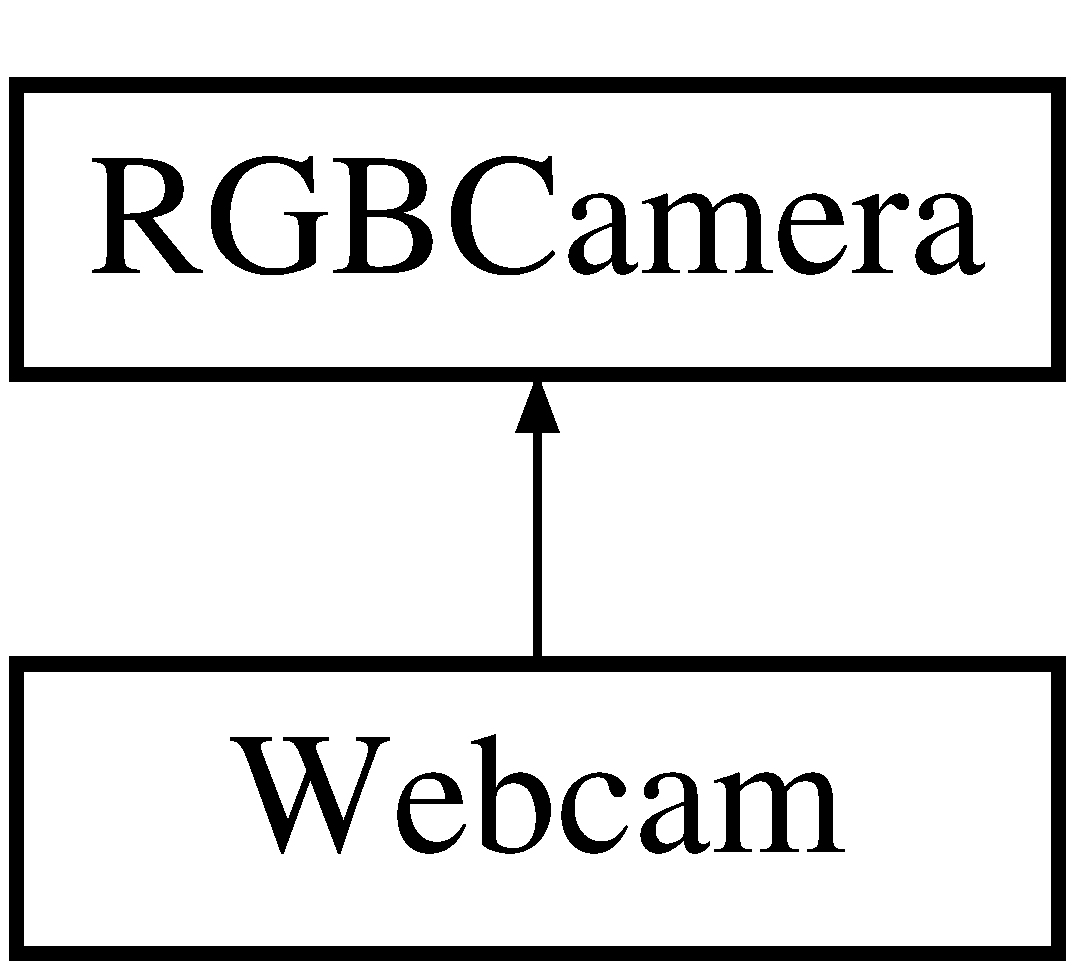
\includegraphics[height=2.000000cm]{class_webcam}
\end{center}
\end{figure}
\subsection*{Public Member Functions}
\begin{DoxyCompactItemize}
\item 
\hyperlink{class_webcam_ae3694760a88e8975940045ec8d4c27ed}{Webcam} (int code=0)
\begin{DoxyCompactList}\small\item\em Constructs a new webcam instance. \end{DoxyCompactList}\item 
\hyperlink{class_webcam_a573d188c6505287dadb895b1ee7526b9}{$\sim$\+Webcam} ()
\begin{DoxyCompactList}\small\item\em Deconstructs a webcam instance. \end{DoxyCompactList}\item 
void \hyperlink{class_webcam_a3d5cab0a2b87b90b85793bc05414e503}{update} ()
\begin{DoxyCompactList}\small\item\em Updates the webcam infomration with the current frame. \end{DoxyCompactList}\end{DoxyCompactItemize}
\subsection*{Additional Inherited Members}


\subsection{Detailed Description}
Class defining the behavior of a standard webcam. 

\subsection{Constructor \& Destructor Documentation}
\hypertarget{class_webcam_ae3694760a88e8975940045ec8d4c27ed}{}\label{class_webcam_ae3694760a88e8975940045ec8d4c27ed} 
\index{Webcam@{Webcam}!Webcam@{Webcam}}
\index{Webcam@{Webcam}!Webcam@{Webcam}}
\subsubsection{\texorpdfstring{Webcam()}{Webcam()}}
{\footnotesize\ttfamily Webcam\+::\+Webcam (\begin{DoxyParamCaption}\item[{int}]{code = {\ttfamily 0} }\end{DoxyParamCaption})}



Constructs a new webcam instance. 


\begin{DoxyParams}{Parameters}
{\em code} & the code for the webcam. Default is 0 if there is only one webcam connected \\
\hline
\end{DoxyParams}
\hypertarget{class_webcam_a573d188c6505287dadb895b1ee7526b9}{}\label{class_webcam_a573d188c6505287dadb895b1ee7526b9} 
\index{Webcam@{Webcam}!````~Webcam@{$\sim$\+Webcam}}
\index{````~Webcam@{$\sim$\+Webcam}!Webcam@{Webcam}}
\subsubsection{\texorpdfstring{$\sim$\+Webcam()}{~Webcam()}}
{\footnotesize\ttfamily Webcam\+::$\sim$\+Webcam (\begin{DoxyParamCaption}{ }\end{DoxyParamCaption})}



Deconstructs a webcam instance. 



\subsection{Member Function Documentation}
\hypertarget{class_webcam_a3d5cab0a2b87b90b85793bc05414e503}{}\label{class_webcam_a3d5cab0a2b87b90b85793bc05414e503} 
\index{Webcam@{Webcam}!update@{update}}
\index{update@{update}!Webcam@{Webcam}}
\subsubsection{\texorpdfstring{update()}{update()}}
{\footnotesize\ttfamily void Webcam\+::update (\begin{DoxyParamCaption}{ }\end{DoxyParamCaption})\hspace{0.3cm}{\ttfamily [virtual]}}



Updates the webcam infomration with the current frame. 



Implements \hyperlink{class_r_g_b_camera_ac9fa3f8f32605e846827b694ae7cff18}{R\+G\+B\+Camera}.



The documentation for this class was generated from the following files\+:\begin{DoxyCompactItemize}
\item 
\hyperlink{_webcam_8h}{Webcam.\+h}\item 
\hyperlink{_webcam_8cpp}{Webcam.\+cpp}\end{DoxyCompactItemize}

\chapter{File Documentation}
\hypertarget{_calibration_8cpp}{}\section{Calibration.\+cpp File Reference}
\label{_calibration_8cpp}\index{Calibration.\+cpp@{Calibration.\+cpp}}
{\ttfamily \#include \char`\"{}Calibration.\+h\char`\"{}}\newline

\hypertarget{_calibration_8h}{}\section{Calibration.\+h File Reference}
\label{_calibration_8h}\index{Calibration.\+h@{Calibration.\+h}}
{\ttfamily \#include $<$fstream$>$}\newline
{\ttfamily \#include $<$opencv/cxcore.\+h$>$}\newline
{\ttfamily \#include $<$opencv/highgui.\+h$>$}\newline
{\ttfamily \#include \char`\"{}opencv2/calib3d/calib3d.\+hpp\char`\"{}}\newline
{\ttfamily \#include \char`\"{}opencv2/highgui/highgui.\+hpp\char`\"{}}\newline
{\ttfamily \#include $<$opencv2/video/tracking.\+hpp$>$}\newline
{\ttfamily \#include \char`\"{}opencv2/imgproc/imgproc.\+hpp\char`\"{}}\newline
{\ttfamily \#include $<$opencv2/objdetect/objdetect.\+hpp$>$}\newline
{\ttfamily \#include $<$opencv2/features2d/features2d.\+hpp$>$}\newline
{\ttfamily \#include $<$Eigen/\+S\+VD$>$}\newline
{\ttfamily \#include \char`\"{}Visualizer.\+h\char`\"{}}\newline
{\ttfamily \#include \char`\"{}Depth\+Camera.\+h\char`\"{}}\newline
{\ttfamily \#include \char`\"{}R\+G\+B\+Camera.\+h\char`\"{}}\newline
{\ttfamily \#include \char`\"{}Util.\+h\char`\"{}}\newline
\subsection*{Classes}
\begin{DoxyCompactItemize}
\item 
class \hyperlink{class_calibration}{Calibration}
\begin{DoxyCompactList}\small\item\em Class for various calibration operations. \end{DoxyCompactList}\end{DoxyCompactItemize}

\hypertarget{_depth_camera_8cpp}{}\section{Depth\+Camera.\+cpp File Reference}
\label{_depth_camera_8cpp}\index{Depth\+Camera.\+cpp@{Depth\+Camera.\+cpp}}
{\ttfamily \#include \char`\"{}Depth\+Camera.\+h\char`\"{}}\newline

\hypertarget{_depth_camera_8h}{}\section{Depth\+Camera.\+h File Reference}
\label{_depth_camera_8h}\index{Depth\+Camera.\+h@{Depth\+Camera.\+h}}
{\ttfamily \#include $<$iostream$>$}\newline
{\ttfamily \#include $<$opencv/cxcore.\+h$>$}\newline
{\ttfamily \#include $<$opencv/highgui.\+h$>$}\newline
{\ttfamily \#include \char`\"{}opencv2/highgui/highgui.\+hpp\char`\"{}}\newline
{\ttfamily \#include $<$opencv2/video/tracking.\+hpp$>$}\newline
{\ttfamily \#include \char`\"{}opencv2/imgproc/imgproc.\+hpp\char`\"{}}\newline
{\ttfamily \#include $<$opencv2/objdetect/objdetect.\+hpp$>$}\newline
{\ttfamily \#include $<$opencv2/features2d/features2d.\+hpp$>$}\newline
{\ttfamily \#include \char`\"{}Util.\+h\char`\"{}}\newline
\subsection*{Classes}
\begin{DoxyCompactItemize}
\item 
class \hyperlink{class_depth_camera}{Depth\+Camera}
\begin{DoxyCompactList}\small\item\em Class defining general behavior of a depth camera. \end{DoxyCompactList}\end{DoxyCompactItemize}

\hypertarget{_hand_8cpp}{}\section{Hand.\+cpp File Reference}
\label{_hand_8cpp}\index{Hand.\+cpp@{Hand.\+cpp}}
{\ttfamily \#include \char`\"{}Hand.\+h\char`\"{}}\newline
{\ttfamily \#include \char`\"{}Util.\+h\char`\"{}}\newline
{\ttfamily \#include \char`\"{}Visualizer.\+h\char`\"{}}\newline

\hypertarget{_hand_8h}{}\section{Hand.\+h File Reference}
\label{_hand_8h}\index{Hand.\+h@{Hand.\+h}}
{\ttfamily \#include $<$iostream$>$}\newline
{\ttfamily \#include $<$vector$>$}\newline
{\ttfamily \#include $<$cmath$>$}\newline
{\ttfamily \#include $<$opencv2/core/core.\+hpp$>$}\newline
{\ttfamily \#include $<$opencv2/core.\+hpp$>$}\newline
{\ttfamily \#include $<$opencv2/highgui/highgui.\+hpp$>$}\newline
{\ttfamily \#include $<$opencv2/highgui.\+hpp$>$}\newline
{\ttfamily \#include $<$opencv2/imgproc.\+hpp$>$}\newline
{\ttfamily \#include $<$opencv2/imgcodecs.\+hpp$>$}\newline
\subsection*{Classes}
\begin{DoxyCompactItemize}
\item 
class \hyperlink{class_hand}{Hand}
\end{DoxyCompactItemize}

\hypertarget{main_8cpp}{}\section{main.\+cpp File Reference}
\label{main_8cpp}\index{main.\+cpp@{main.\+cpp}}
{\ttfamily \#include $<$stdio.\+h$>$}\newline
{\ttfamily \#include $<$iostream$>$}\newline
{\ttfamily \#include $<$string$>$}\newline
{\ttfamily \#include $<$time.\+h$>$}\newline
{\ttfamily \#include $<$opencv/cxcore.\+h$>$}\newline
{\ttfamily \#include \char`\"{}opencv2/highgui/highgui.\+hpp\char`\"{}}\newline
{\ttfamily \#include \char`\"{}P\+M\+D\+Camera.\+h\char`\"{}}\newline
{\ttfamily \#include \char`\"{}Webcam.\+h\char`\"{}}\newline
{\ttfamily \#include \char`\"{}Visualizer.\+h\char`\"{}}\newline
{\ttfamily \#include \char`\"{}Hand.\+h\char`\"{}}\newline
{\ttfamily \#include \char`\"{}Plane.\+h\char`\"{}}\newline
{\ttfamily \#include \char`\"{}Calibration.\+h\char`\"{}}\newline
{\ttfamily \#include \char`\"{}Util.\+h\char`\"{}}\newline
{\ttfamily \#include \char`\"{}U\+D\+P\+Sender.\+h\char`\"{}}\newline
{\ttfamily \#include \char`\"{}Object3\+D.\+h\char`\"{}}\newline
{\ttfamily \#include \char`\"{}Streaming\+Averager.\+h\char`\"{}}\newline
\subsection*{Functions}
\begin{DoxyCompactItemize}
\item 
int \hyperlink{main_8cpp_ae66f6b31b5ad750f1fe042a706a4e3d4}{main} ()
\end{DoxyCompactItemize}


\subsection{Function Documentation}
\hypertarget{main_8cpp_ae66f6b31b5ad750f1fe042a706a4e3d4}{}\label{main_8cpp_ae66f6b31b5ad750f1fe042a706a4e3d4} 
\index{main.\+cpp@{main.\+cpp}!main@{main}}
\index{main@{main}!main.\+cpp@{main.\+cpp}}
\subsubsection{\texorpdfstring{main()}{main()}}
{\footnotesize\ttfamily int main (\begin{DoxyParamCaption}{ }\end{DoxyParamCaption})}

std\+::string filename = \char`\"{}..//\+Open\+A\+R\+K\+\_\+\+Datasets//\+Two\+Hand\+Data\+Set1//img\char`\"{} + std\+::to\+\_\+string(frame) + \char`\"{}.\+yml\char`\"{}; if (!pmd-\/$>$read\+Image(filename)) break;
\hypertarget{_plane_8cpp}{}\section{Plane.\+cpp File Reference}
\label{_plane_8cpp}\index{Plane.\+cpp@{Plane.\+cpp}}
{\ttfamily \#include \char`\"{}Plane.\+h\char`\"{}}\newline

\hypertarget{_plane_8h}{}\section{Plane.\+h File Reference}
\label{_plane_8h}\index{Plane.\+h@{Plane.\+h}}
{\ttfamily \#include $<$iostream$>$}\newline
{\ttfamily \#include $<$cstdio$>$}\newline
{\ttfamily \#include $<$ctime$>$}\newline
{\ttfamily \#include $<$opencv2/highgui/highgui.\+hpp$>$}\newline
{\ttfamily \#include $<$opencv2/core/core.\+hpp$>$}\newline
{\ttfamily \#include $<$opencv2/imgproc/imgproc.\+hpp$>$}\newline
{\ttfamily \#include $<$pcl/filters/voxel\+\_\+grid.\+h$>$}\newline
{\ttfamily \#include $<$pcl/point\+\_\+types.\+h$>$}\newline
{\ttfamily \#include $<$pcl/features/normal\+\_\+3d.\+h$>$}\newline
{\ttfamily \#include $<$pcl/io/pcd\+\_\+io.\+h$>$}\newline
{\ttfamily \#include $<$pcl/io/ply\+\_\+io.\+h$>$}\newline
{\ttfamily \#include $<$pcl/point\+\_\+cloud.\+h$>$}\newline
{\ttfamily \#include $<$pcl/console/parse.\+h$>$}\newline
{\ttfamily \#include $<$pcl/common/transforms.\+h$>$}\newline
{\ttfamily \#include $<$pcl/visualization/pcl\+\_\+visualizer.\+h$>$}\newline
{\ttfamily \#include $<$pcl/filters/passthrough.\+h$>$}\newline
{\ttfamily \#include $<$pcl/features/integral\+\_\+image\+\_\+normal.\+h$>$}\newline
{\ttfamily \#include $<$pcl/visualization/cloud\+\_\+viewer.\+h$>$}\newline
{\ttfamily \#include $<$pcl/segmentation/region\+\_\+growing.\+h$>$}\newline
{\ttfamily \#include $<$pcl/features/normal\+\_\+3d\+\_\+omp.\+h$>$}\newline
\subsection*{Classes}
\begin{DoxyCompactItemize}
\item 
class \hyperlink{class_plane}{Plane}
\begin{DoxyCompactList}\small\item\em Class defining a plane object. \end{DoxyCompactList}\end{DoxyCompactItemize}

\hypertarget{_p_m_d_camera_8cpp}{}\section{P\+M\+D\+Camera.\+cpp File Reference}
\label{_p_m_d_camera_8cpp}\index{P\+M\+D\+Camera.\+cpp@{P\+M\+D\+Camera.\+cpp}}
{\ttfamily \#include \char`\"{}P\+M\+D\+Camera.\+h\char`\"{}}\newline

\hypertarget{_p_m_d_camera_8h}{}\section{P\+M\+D\+Camera.\+h File Reference}
\label{_p_m_d_camera_8h}\index{P\+M\+D\+Camera.\+h@{P\+M\+D\+Camera.\+h}}
{\ttfamily \#include $<$string.\+h$>$}\newline
{\ttfamily \#include $<$pmdsdk2.\+h$>$}\newline
{\ttfamily \#include $<$opencv/cxcore.\+h$>$}\newline
{\ttfamily \#include $<$opencv/highgui.\+h$>$}\newline
{\ttfamily \#include \char`\"{}opencv2/highgui/highgui.\+hpp\char`\"{}}\newline
{\ttfamily \#include $<$opencv2/video/tracking.\+hpp$>$}\newline
{\ttfamily \#include \char`\"{}opencv2/imgproc/imgproc.\+hpp\char`\"{}}\newline
{\ttfamily \#include $<$opencv2/objdetect/objdetect.\+hpp$>$}\newline
{\ttfamily \#include $<$opencv2/features2d/features2d.\+hpp$>$}\newline
{\ttfamily \#include \char`\"{}Depth\+Camera.\+h\char`\"{}}\newline
\subsection*{Classes}
\begin{DoxyCompactItemize}
\item 
class \hyperlink{class_p_m_d_camera}{P\+M\+D\+Camera}
\begin{DoxyCompactList}\small\item\em Class defining the behavior of a P\+MD Camera. \end{DoxyCompactList}\end{DoxyCompactItemize}

\hypertarget{_open_a_r_k-_s_d_k_2_r_e_a_d_m_e_8md}{}\section{R\+E\+A\+D\+M\+E.\+md File Reference}
\label{_open_a_r_k-_s_d_k_2_r_e_a_d_m_e_8md}\index{R\+E\+A\+D\+M\+E.\+md@{R\+E\+A\+D\+M\+E.\+md}}

\hypertarget{_r_e_a_d_m_e_8md}{}\section{R\+E\+A\+D\+M\+E.\+md File Reference}
\label{_r_e_a_d_m_e_8md}\index{R\+E\+A\+D\+M\+E.\+md@{R\+E\+A\+D\+M\+E.\+md}}

\hypertarget{_r_g_b_camera_8cpp}{}\section{R\+G\+B\+Camera.\+cpp File Reference}
\label{_r_g_b_camera_8cpp}\index{R\+G\+B\+Camera.\+cpp@{R\+G\+B\+Camera.\+cpp}}
{\ttfamily \#include \char`\"{}R\+G\+B\+Camera.\+h\char`\"{}}\newline

\hypertarget{_r_g_b_camera_8h}{}\section{R\+G\+B\+Camera.\+h File Reference}
\label{_r_g_b_camera_8h}\index{R\+G\+B\+Camera.\+h@{R\+G\+B\+Camera.\+h}}
{\ttfamily \#include $<$opencv/cxcore.\+h$>$}\newline
{\ttfamily \#include \char`\"{}opencv2/highgui/highgui.\+hpp\char`\"{}}\newline
\subsection*{Classes}
\begin{DoxyCompactItemize}
\item 
class \hyperlink{class_r_g_b_camera}{R\+G\+B\+Camera}
\begin{DoxyCompactList}\small\item\em Abstract class that defines the behavior of a R\+GB camera. \end{DoxyCompactList}\end{DoxyCompactItemize}

\hypertarget{_sensor_i_o_8cpp}{}\section{Sensor\+I\+O.\+cpp File Reference}
\label{_sensor_i_o_8cpp}\index{Sensor\+I\+O.\+cpp@{Sensor\+I\+O.\+cpp}}
{\ttfamily \#include $<$stdio.\+h$>$}\newline
{\ttfamily \#include $<$iostream$>$}\newline
{\ttfamily \#include $<$string$>$}\newline
{\ttfamily \#include $<$opencv/cxcore.\+h$>$}\newline
{\ttfamily \#include \char`\"{}opencv2/highgui/highgui.\+hpp\char`\"{}}\newline
{\ttfamily \#include \char`\"{}P\+M\+D\+Camera.\+h\char`\"{}}\newline
{\ttfamily \#include \char`\"{}Visualizer.\+h\char`\"{}}\newline
{\ttfamily \#include \char`\"{}Util.\+h\char`\"{}}\newline
\subsection*{Functions}
\begin{DoxyCompactItemize}
\item 
int \hyperlink{_sensor_i_o_8cpp_ae66f6b31b5ad750f1fe042a706a4e3d4}{main} ()
\end{DoxyCompactItemize}


\subsection{Function Documentation}
\hypertarget{_sensor_i_o_8cpp_ae66f6b31b5ad750f1fe042a706a4e3d4}{}\label{_sensor_i_o_8cpp_ae66f6b31b5ad750f1fe042a706a4e3d4} 
\index{Sensor\+I\+O.\+cpp@{Sensor\+I\+O.\+cpp}!main@{main}}
\index{main@{main}!Sensor\+I\+O.\+cpp@{Sensor\+I\+O.\+cpp}}
\subsubsection{\texorpdfstring{main()}{main()}}
{\footnotesize\ttfamily int main (\begin{DoxyParamCaption}{ }\end{DoxyParamCaption})}


\hypertarget{_u_d_p_sender_8cpp}{}\section{U\+D\+P\+Sender.\+cpp File Reference}
\label{_u_d_p_sender_8cpp}\index{U\+D\+P\+Sender.\+cpp@{U\+D\+P\+Sender.\+cpp}}
{\ttfamily \#include \char`\"{}U\+D\+P\+Sender.\+h\char`\"{}}\newline
\subsection*{Macros}
\begin{DoxyCompactItemize}
\item 
\#define \hyperlink{_u_d_p_sender_8cpp_adfc8f90f3a8caa8423099cf36ff214f1}{\+\_\+\+W\+I\+N\+S\+O\+C\+K\+\_\+\+D\+E\+P\+R\+E\+C\+A\+T\+E\+D\+\_\+\+N\+O\+\_\+\+W\+A\+R\+N\+I\+N\+GS}
\end{DoxyCompactItemize}


\subsection{Macro Definition Documentation}
\hypertarget{_u_d_p_sender_8cpp_adfc8f90f3a8caa8423099cf36ff214f1}{}\label{_u_d_p_sender_8cpp_adfc8f90f3a8caa8423099cf36ff214f1} 
\index{U\+D\+P\+Sender.\+cpp@{U\+D\+P\+Sender.\+cpp}!\+\_\+\+W\+I\+N\+S\+O\+C\+K\+\_\+\+D\+E\+P\+R\+E\+C\+A\+T\+E\+D\+\_\+\+N\+O\+\_\+\+W\+A\+R\+N\+I\+N\+GS@{\+\_\+\+W\+I\+N\+S\+O\+C\+K\+\_\+\+D\+E\+P\+R\+E\+C\+A\+T\+E\+D\+\_\+\+N\+O\+\_\+\+W\+A\+R\+N\+I\+N\+GS}}
\index{\+\_\+\+W\+I\+N\+S\+O\+C\+K\+\_\+\+D\+E\+P\+R\+E\+C\+A\+T\+E\+D\+\_\+\+N\+O\+\_\+\+W\+A\+R\+N\+I\+N\+GS@{\+\_\+\+W\+I\+N\+S\+O\+C\+K\+\_\+\+D\+E\+P\+R\+E\+C\+A\+T\+E\+D\+\_\+\+N\+O\+\_\+\+W\+A\+R\+N\+I\+N\+GS}!U\+D\+P\+Sender.\+cpp@{U\+D\+P\+Sender.\+cpp}}
\subsubsection{\texorpdfstring{\+\_\+\+W\+I\+N\+S\+O\+C\+K\+\_\+\+D\+E\+P\+R\+E\+C\+A\+T\+E\+D\+\_\+\+N\+O\+\_\+\+W\+A\+R\+N\+I\+N\+GS}{\_WINSOCK\_DEPRECATED\_NO\_WARNINGS}}
{\footnotesize\ttfamily \#define \+\_\+\+W\+I\+N\+S\+O\+C\+K\+\_\+\+D\+E\+P\+R\+E\+C\+A\+T\+E\+D\+\_\+\+N\+O\+\_\+\+W\+A\+R\+N\+I\+N\+GS}


\hypertarget{_u_d_p_sender_8h}{}\section{U\+D\+P\+Sender.\+h File Reference}
\label{_u_d_p_sender_8h}\index{U\+D\+P\+Sender.\+h@{U\+D\+P\+Sender.\+h}}
{\ttfamily \#include $<$winsock2.\+h$>$}\newline
{\ttfamily \#include $<$stdio.\+h$>$}\newline
{\ttfamily \#include $<$iostream$>$}\newline
\subsection*{Classes}
\begin{DoxyCompactItemize}
\item 
class \hyperlink{class_u_d_p_sender}{U\+D\+P\+Sender}
\begin{DoxyCompactList}\small\item\em U\+DP client. \end{DoxyCompactList}\end{DoxyCompactItemize}
\subsection*{Macros}
\begin{DoxyCompactItemize}
\item 
\#define \hyperlink{_u_d_p_sender_8h_adfc8f90f3a8caa8423099cf36ff214f1}{\+\_\+\+W\+I\+N\+S\+O\+C\+K\+\_\+\+D\+E\+P\+R\+E\+C\+A\+T\+E\+D\+\_\+\+N\+O\+\_\+\+W\+A\+R\+N\+I\+N\+GS}
\item 
\#define \hyperlink{_u_d_p_sender_8h_a24cd3c37a165a8c4626d9e78df4574ff}{S\+E\+R\+V\+ER}~\char`\"{}127.\+0.\+0.\+1\char`\"{}
\item 
\#define \hyperlink{_u_d_p_sender_8h_ad974fe981249f5e84fbf1683b012c9f8}{B\+U\+F\+L\+EN}~512
\item 
\#define \hyperlink{_u_d_p_sender_8h_a614217d263be1fb1a5f76e2ff7be19a2}{P\+O\+RT}~8051
\end{DoxyCompactItemize}


\subsection{Macro Definition Documentation}
\hypertarget{_u_d_p_sender_8h_adfc8f90f3a8caa8423099cf36ff214f1}{}\label{_u_d_p_sender_8h_adfc8f90f3a8caa8423099cf36ff214f1} 
\index{U\+D\+P\+Sender.\+h@{U\+D\+P\+Sender.\+h}!\+\_\+\+W\+I\+N\+S\+O\+C\+K\+\_\+\+D\+E\+P\+R\+E\+C\+A\+T\+E\+D\+\_\+\+N\+O\+\_\+\+W\+A\+R\+N\+I\+N\+GS@{\+\_\+\+W\+I\+N\+S\+O\+C\+K\+\_\+\+D\+E\+P\+R\+E\+C\+A\+T\+E\+D\+\_\+\+N\+O\+\_\+\+W\+A\+R\+N\+I\+N\+GS}}
\index{\+\_\+\+W\+I\+N\+S\+O\+C\+K\+\_\+\+D\+E\+P\+R\+E\+C\+A\+T\+E\+D\+\_\+\+N\+O\+\_\+\+W\+A\+R\+N\+I\+N\+GS@{\+\_\+\+W\+I\+N\+S\+O\+C\+K\+\_\+\+D\+E\+P\+R\+E\+C\+A\+T\+E\+D\+\_\+\+N\+O\+\_\+\+W\+A\+R\+N\+I\+N\+GS}!U\+D\+P\+Sender.\+h@{U\+D\+P\+Sender.\+h}}
\subsubsection{\texorpdfstring{\+\_\+\+W\+I\+N\+S\+O\+C\+K\+\_\+\+D\+E\+P\+R\+E\+C\+A\+T\+E\+D\+\_\+\+N\+O\+\_\+\+W\+A\+R\+N\+I\+N\+GS}{\_WINSOCK\_DEPRECATED\_NO\_WARNINGS}}
{\footnotesize\ttfamily \#define \+\_\+\+W\+I\+N\+S\+O\+C\+K\+\_\+\+D\+E\+P\+R\+E\+C\+A\+T\+E\+D\+\_\+\+N\+O\+\_\+\+W\+A\+R\+N\+I\+N\+GS}

\hypertarget{_u_d_p_sender_8h_ad974fe981249f5e84fbf1683b012c9f8}{}\label{_u_d_p_sender_8h_ad974fe981249f5e84fbf1683b012c9f8} 
\index{U\+D\+P\+Sender.\+h@{U\+D\+P\+Sender.\+h}!B\+U\+F\+L\+EN@{B\+U\+F\+L\+EN}}
\index{B\+U\+F\+L\+EN@{B\+U\+F\+L\+EN}!U\+D\+P\+Sender.\+h@{U\+D\+P\+Sender.\+h}}
\subsubsection{\texorpdfstring{B\+U\+F\+L\+EN}{BUFLEN}}
{\footnotesize\ttfamily \#define B\+U\+F\+L\+EN~512}

\hypertarget{_u_d_p_sender_8h_a614217d263be1fb1a5f76e2ff7be19a2}{}\label{_u_d_p_sender_8h_a614217d263be1fb1a5f76e2ff7be19a2} 
\index{U\+D\+P\+Sender.\+h@{U\+D\+P\+Sender.\+h}!P\+O\+RT@{P\+O\+RT}}
\index{P\+O\+RT@{P\+O\+RT}!U\+D\+P\+Sender.\+h@{U\+D\+P\+Sender.\+h}}
\subsubsection{\texorpdfstring{P\+O\+RT}{PORT}}
{\footnotesize\ttfamily \#define P\+O\+RT~8051}

\hypertarget{_u_d_p_sender_8h_a24cd3c37a165a8c4626d9e78df4574ff}{}\label{_u_d_p_sender_8h_a24cd3c37a165a8c4626d9e78df4574ff} 
\index{U\+D\+P\+Sender.\+h@{U\+D\+P\+Sender.\+h}!S\+E\+R\+V\+ER@{S\+E\+R\+V\+ER}}
\index{S\+E\+R\+V\+ER@{S\+E\+R\+V\+ER}!U\+D\+P\+Sender.\+h@{U\+D\+P\+Sender.\+h}}
\subsubsection{\texorpdfstring{S\+E\+R\+V\+ER}{SERVER}}
{\footnotesize\ttfamily \#define S\+E\+R\+V\+ER~\char`\"{}127.\+0.\+0.\+1\char`\"{}}


\hypertarget{_util_8cpp}{}\section{Util.\+cpp File Reference}
\label{_util_8cpp}\index{Util.\+cpp@{Util.\+cpp}}
{\ttfamily \#include \char`\"{}Util.\+h\char`\"{}}\newline

\hypertarget{_util_8h}{}\section{Util.\+h File Reference}
\label{_util_8h}\index{Util.\+h@{Util.\+h}}
{\ttfamily \#include $<$opencv/cxcore.\+h$>$}\newline
\subsection*{Classes}
\begin{DoxyCompactItemize}
\item 
class \hyperlink{class_util}{Util}
\begin{DoxyCompactList}\small\item\em Class containing generic helper functions. \end{DoxyCompactList}\end{DoxyCompactItemize}
\subsection*{Macros}
\begin{DoxyCompactItemize}
\item 
\#define \hyperlink{_util_8h_ae71449b1cc6e6250b91f539153a7a0d3}{M\+\_\+\+PI}~3.\+14159265358979323846
\end{DoxyCompactItemize}


\subsection{Macro Definition Documentation}
\hypertarget{_util_8h_ae71449b1cc6e6250b91f539153a7a0d3}{}\label{_util_8h_ae71449b1cc6e6250b91f539153a7a0d3} 
\index{Util.\+h@{Util.\+h}!M\+\_\+\+PI@{M\+\_\+\+PI}}
\index{M\+\_\+\+PI@{M\+\_\+\+PI}!Util.\+h@{Util.\+h}}
\subsubsection{\texorpdfstring{M\+\_\+\+PI}{M\_PI}}
{\footnotesize\ttfamily \#define M\+\_\+\+PI~3.\+14159265358979323846}


\hypertarget{_visualizer_8cpp}{}\section{Visualizer.\+cpp File Reference}
\label{_visualizer_8cpp}\index{Visualizer.\+cpp@{Visualizer.\+cpp}}
{\ttfamily \#include \char`\"{}Visualizer.\+h\char`\"{}}\newline

\hypertarget{_visualizer_8h}{}\section{Visualizer.\+h File Reference}
\label{_visualizer_8h}\index{Visualizer.\+h@{Visualizer.\+h}}
{\ttfamily \#include $<$opencv2/core/core.\+hpp$>$}\newline
{\ttfamily \#include $<$opencv2/highgui/highgui.\+hpp$>$}\newline
{\ttfamily \#include $<$opencv2/core.\+hpp$>$}\newline
{\ttfamily \#include $<$opencv2/imgproc.\+hpp$>$}\newline
{\ttfamily \#include $<$opencv2/imgcodecs.\+hpp$>$}\newline
{\ttfamily \#include $<$opencv2/highgui.\+hpp$>$}\newline
{\ttfamily \#include $<$pcl/point\+\_\+types.\+h$>$}\newline
{\ttfamily \#include $<$pcl/io/pcd\+\_\+io.\+h$>$}\newline
{\ttfamily \#include $<$pcl/kdtree/kdtree\+\_\+flann.\+h$>$}\newline
{\ttfamily \#include $<$pcl/features/normal\+\_\+3d.\+h$>$}\newline
{\ttfamily \#include $<$pcl/surface/gp3.\+h$>$}\newline
{\ttfamily \#include $<$pcl/visualization/cloud\+\_\+viewer.\+h$>$}\newline
\subsection*{Classes}
\begin{DoxyCompactItemize}
\item 
class \hyperlink{class_visualizer}{Visualizer}
\begin{DoxyCompactList}\small\item\em Utility class containing various conversions and visualization techniques. \end{DoxyCompactList}\end{DoxyCompactItemize}

\hypertarget{_webcam_8cpp}{}\section{Webcam.\+cpp File Reference}
\label{_webcam_8cpp}\index{Webcam.\+cpp@{Webcam.\+cpp}}
{\ttfamily \#include \char`\"{}Webcam.\+h\char`\"{}}\newline

\hypertarget{_webcam_8h}{}\section{Webcam.\+h File Reference}
\label{_webcam_8h}\index{Webcam.\+h@{Webcam.\+h}}
{\ttfamily \#include \char`\"{}R\+G\+B\+Camera.\+h\char`\"{}}\newline
\subsection*{Classes}
\begin{DoxyCompactItemize}
\item 
class \hyperlink{class_webcam}{Webcam}
\begin{DoxyCompactList}\small\item\em Class defining the behavior of a standard webcam. \end{DoxyCompactList}\end{DoxyCompactItemize}

%--- End generated contents ---

% Index
\backmatter
\newpage
\phantomsection
\clearemptydoublepage
\addcontentsline{toc}{chapter}{Index}
\printindex

\end{document}
